%!TEX root = ../larxxia.tex


\section{Find eigenvalues and eigenvectors of matrices}
\label{sec:eennm}
\index{eigenvalue|(}
\index{eigenvector|(}

\secttoc
\begin{comment}
\pooliv{\S4.3}  \layiv{\S5.2} \holti{\S6.1}  \cite[Ch.~9]{Chartier2015}.
\end{comment}


This section begins exploring the properties and some applications of the \idx{eigen-problem} \(A\xv=\lambda\xv\) for \emph{general} matrices~\(A\).
The section generalises properties established for symmetric matrices, \cref{ch:eesm}, and relies on the determinant methods of \cref{ch:ddm}.
We establish that there are generally \(n\)~eigenvalues of an \(n\times n\) matrix, albeit possibly non-real complex valued, and also that \idx{repeated eigenvalue}s are sensitive to errors.
Applications include population modelling,  
the computation of \svd{}s\ifcsname r@sec:eidd\endcsname, and 
fitting exponential functions to real data\fi.




\subsection{A characteristic equation gives eigenvalues}
\label{sec:cege}

\index{characteristic equation|(}
\begin{quoted}{J.~H. Wilkinson, 1984 \cite[p.103]{Higham1996}}
The \idx{Fundamental Theorem of Algebra} asserts that every polynomial equation over the complex field has a root.  
It is almost beneath the dignity of such a majestic theorem to mention that in fact it has precisely \(n\)~roots.
\end{quoted}


Recall that eigenvalues~\(\lambda\) and nonzero eigenvectors~\xv\ of a square matrix~\(A\) must satisfy \((A-\lambda I)\xv=\ov\)\,.
\cref{thm:detinv} then implies the \idx{eigenvalue}s of a \idx{square matrix} are precisely the solutions of the \bfidx{characteristic equation} \(\det(A-\lambda I)=0\)\,.  

\begin{theorem} \label{thm:geecp}
For every \(n\times n\) \idx{square matrix}~\(A\) we call \(\det(A-\lambda I)\) the \bfidx{characteristic polynomial} of~\(A\):%
\footnote{Alternatively, many call \(\det(\lambda I-A)\) the characteristic polynomial, as does \script.  
The distinction is immaterial as,  for an \(n\times n\) matrix~\(A\) and by \cref{thm:basicdet:iii} with multiplicative factor \(k=-1\)\,, the only difference in the \idx{determinant} is a factor of~\((-1)^n\).
In \script, \index{poly()@\texttt{poly()}}\texttt{poly(A)} computes the characteristic polynomial of the matrix,  \(\det(\lambda I-A)\), which might be useful for exercises, but is rarely useful in practice due to poor conditioning.}
\begin{itemize}
\item the \idx{characteristic polynomial} of~\(A\) is a polynomial of \(n\)th~degree in~\(\lambda\);
\item  there are at most \(n\)~\idx{distinct eigenvalues} of~\(A\).
\end{itemize}
\end{theorem}

\begin{proof} 
% Do not do this as we want the induction for the next theorem's proof.
%Consider the characteristic polynomial
%\begin{equation*}
%\det(A-\lambda I)=
%\det\begin{bmatrix} a_{11}-\lambda&a_{12}&\cdots&a_{1n}
%\\a_{21}&a_{22}-\lambda&&a_{2n}
%\\\vdots&&\ddots&\vdots
%\\a_{n1}&a_{n2}&\cdots&a_{nn}-\lambda \end{bmatrix}.
%\end{equation*}
%Recall \cref{thm:detnfac} asserts that the determinant of an \(n\times n\) matrix is a sum of \(n!\)~terms where each term is a product of \(n\)~factors where each factor in a term comes from a different row and column of the matrix.
%Being a sum of products of these entries, \(\det(A-\lambda I)\) is a polynomial in~\(\lambda\).
%Since each term is a product of \(n\)~factors, and each factor is an entry in the matrix~\(A-\lambda I\)\,, and each entry is at most linear in~\(\lambda\), then the polynomial is of degree at most~\(n\) in~\(\lambda\).
%One of the \(n!\)~terms in the sum is the product along the diagonal \((a_{11}-\lambda)(a_{22}-\lambda)\cdots(a_{nn}-\lambda)\): consequently the polynomial has a term in~\(\lambda^n\) and so is of degree~\(n\).
Use induction on the size of the matrix.
First, for \(1\times 1\) matrix \(A=\begin{bmatrix} a_{11} \end{bmatrix}\), the determinant \(\det(A-\lambda I)=\det \begin{bmatrix} a_{11}-\lambda \end{bmatrix}=a_{11}-\lambda\) which is of  degree one in~\(\lambda\).
Second, assume that for every \((n-1)\times (n-1)\) matrix~\(A\), \(\det(A-\lambda I)\) is a polynomial of degree~\(n-1\) in~\(\lambda\).
Consider any \(n\times n\) matrix~\(A\).
Use the Laplace Expansion \cref{thm:letdet} to give the first row expansion, in terms of minors of~\(A\) and~\(I\),
\begin{eqnarray*}
\det(A-\lambda I)
&=&(a_{11}-\lambda)\det (A_{11}-\lambda I_{11})
-a_{12}\det (A_{12}-\lambda I_{12})
\\&&{}
+\cdots-(-1)^{n}a_{1n}\det (A_{1n}-\lambda I_{1n}).
\end{eqnarray*}
Now the minor~\(I_{11}\) is precisely the \((n-1)\times(n-1)\) identity, and hence by assumption \(\det(A_{11}-\lambda I_{11})\) is a polynomial of degree~\((n-1)\) in~\(\lambda\).
But differently, the minors~\(I_{12},\ldots,I_{1n}\) have two of the ones removed from the \(n\times n\)~identity and hence \(\lambda I_{12},\ldots,\lambda I_{1n}\) each have only \((n-2)\)~\(\lambda\)s: since each term in a determinant is a product of distinct entries of the matrix (\cref{thm:detnfac}) it follows that for \(j\geq2\) the determinant \(\det(A_{1j}-\lambda I_{1j})\) is a polynomial in~\(\lambda\) of degree\({}\leq n-2\)\,.
Consequently, the first row expansion of 
\begin{eqnarray*}
\det(A-\lambda I)
&=&(a_{11}-\lambda)(\text{poly degree }n-1)
-a_{12}(\text{poly degree }\leq n-2)
\\&&{}
+\cdots-(-1)^{n}a_{1n}(\text{poly degree }\leq n-2)
\\&=&(a_{11}-\lambda)(\text{poly degree }n-1)
+(\text{poly degree }\leq n-2)
\\&=&(\text{poly degree }n)
\end{eqnarray*}
as the highest power of~\(\lambda\) cannot be cancelled by any term.
Induction thus implies that for every~\(n\) the characteristic polynomial of an \(n\times n\) matrix~\(A\) is a polynomial of \(n\)th~degree in~\(\lambda\).

Lastly, because the characteristic polynomial of~\(A\) is of \(n\)th~degree in~\(\lambda\), the \idx{Fundamental Theorem of Algebra} (established in more advanced courses) asserts that the polynomial has at most \(n\)~roots (possibly complex).  
Hence there are at most \(n\)~distinct eigenvalues (allowing non-real complex eigenvalues).
\end{proof}



\begin{activity}
A given matrix has eigenvalues of~\(-7\), \(-1\), \(3\), \(4\)  and~\(6\).
The matrix must be of \idx{size} \(n\times n\) for~\(n\) at least which of the following? (Select the smallest valid answer.)
\actposs[4]5467
\end{activity}



\begin{example} 
Find the \idx{characteristic polynomial} of each of the following matrices.  
Where in the \idx{coefficient}s of the polynomial can you see the \idx{determinant}? and the sum of the diagonal \idx{elements}?
\begin{enumerate}
\item \(\eAii=\begin{bmatrix} 1&-1\\-2&4 \end{bmatrix}\)
\begin{solution} 
The characteristic polynomial is \(\det(\eAii-\lambda I)
=\det\begin{bmat} 1-\lambda&-1\\-2&4-\lambda \end{bmat}
=(1-\lambda)(4-\lambda)-2
=\lambda^2-5\lambda+2\)\,.
Now \(\det \eAii=4-2=2\) which is the coefficient of the constant term in this polynomial.
Whereas the sum of the diagonal of~\(\eAii\) is \(1+4=5\) which is the negative of the \(\lambda\)~coefficient in \text{the polynomial.}
\end{solution}

\item \(\eAii=\begin{bmatrix}4&-2&1
\\1&-2&0
\\8&2&6 \end{bmatrix}\)
\begin{solution} 
The characteristic polynomial is 
\begin{eqnarray*}
\det(\eAii-\lambda I)
&=&\det\begin{bmatrix} 4-\lambda&-2&1
\\1&-2-\lambda&0
\\8&2&6-\lambda \end{bmatrix}
\\&=&(4-\lambda)(-2-\lambda)(6-\lambda)+0+2
-(-2-\lambda)8-0-(-2)(6-\lambda)
\\&=&-48+4\lambda+8\lambda^2-\lambda^3+2
+16+8\lambda+12+2\lambda
\\&=&-\lambda^3+8\lambda^2+2\lambda-18\,.
\end{eqnarray*}
Now \(\det \eAii=4(-2)6+0+2-(-2)8-0-(-2)6=-48+2+16+12=-18\) which is the coefficient of the constant term in the polynomial.
Whereas the sum of the diagonal of~\(\eAii\) is \(4-2+6=8\) which is the \(\lambda^2\)~coefficient in the polynomial.
\end{solution}

\end{enumerate}
\end{example}




These observations about the \idx{coefficient}s in the characteristic polynomials leads to the next (optional) theorem that helps establish the nature of a characteristic polynomial.

\begin{theorem} \label{thm:charpolyc}
For every \(n\times n\) matrix~\(A\), the product of the \idx{eigenvalue}s equals~\(\det A\), and also equals the \idx{constant term} in the \idx{characteristic polynomial}.  
The \idx{sum} of the \idx{eigenvalue}s equals \((-1)^{n-1}\)~times the \idx{coefficient} of~\(\lambda^{n-1}\) in the \idx{characteristic polynomial}, and also equals the \bfidx{trace} of the matrix, defined as the sum of the diagonal \idx{elements} \(a_{11}+a_{22}+\cdots+a_{nn}\)\,.
% that is, \(\sum_{j=1}^n a_{jj}\).
\end{theorem}

\begin{proof} 
\cref{thm:geecp}, and its proof, establishes that the characteristic polynomial has the form
\begin{align}
\det(A-\lambda I)&=c_0+c_1\lambda+\cdots+c_{n-1}\lambda^{n-1}+(-1)^n\lambda^n
\nonumber\\&=(\lambda_1-\lambda)(\lambda_2-\lambda)\cdots(\lambda_n-\lambda),
\label{eq:charpolyc}
\end{align}
where the second equality follows from the \idx{Fundamental Theorem of Algebra} that an \(n\)th~degree polynomial factors into \(n\)~linear factors (albeit possibly complex).
First, substitute \(\lambda=0\) and this equation~\eqref{eq:charpolyc} gives \(\det A=c_0=\lambda_1\lambda_2\cdots\lambda_n\)\,, \text{as required.}

Second, consider the term~\(c_{n-1}\lambda^{n-1}\) in equation~\eqref{eq:charpolyc}.
From the factorization on the right-hand side, the \(\lambda^{n-1}\)~term arises as
\begin{eqnarray*}
c_{n-1}\lambda^{n-1}&=&\lambda_1(-\lambda)^{n-1}
+(-\lambda)\lambda_2(-\lambda)^{n-2}
+\cdots+(-\lambda)^{n-1}\lambda_n
\\&=&(-1)^{n-1}(\lambda_1+\lambda_2+\cdots+\lambda_n)\lambda^{n-1},
\end{eqnarray*}
and hence the coefficient \(c_{n-1}=(-1)^{n-1}(\lambda_1+\lambda_2+\cdots+\lambda_n)\), as required.
Now use induction to prove the trace formula.
Recall that the proof of \cref{thm:geecp} establishes that
\begin{eqnarray*}
\det(A-\lambda I)
&=&(a_{11}-\lambda)\det (A_{11}-\lambda I_{11})
\\&&{}
+(\text{poly degree }\leq n-2).
\end{eqnarray*}
Assume the trace formula holds for \((n-1)\times(n-1)\) matrices, and so it holds for the minor~\(A_{11}\). 
Then the previous identity gives
\begin{eqnarray*}
\det(A-\lambda I)
&=&(a_{11}-\lambda)\big[(-1)^{n-1}\lambda^{n-1}
+(-1)^{n-2}(a_{22}+\cdots+a_{nn})\lambda^{n-2} 
\\&&\quad{}
+(\text{poly degree }\leq n-3)\big]
+(\text{poly degree }\leq n-2)
\\&=&(-1)^{n}\lambda^{n}
+(-1)^{n-1}(a_{11}+a_{22}+\cdots+a_{nn})\lambda^{n-1} 
+(\text{poly degree }\leq n-2).
\end{eqnarray*}
Hence the coefficient \(c_{n-1}=(-1)^{n-1}(a_{11}+a_{22}+\cdots+a_{nn})\).
Since the formula holds for the basic case \(n=1\), namely \(c_0=+a_{11}\)\,, induction implies the sum of the eigenvalues
\(\lambda_1+\lambda_2+\cdots+\lambda_n=a_{11}+a_{22}+\cdots+a_{nn}\)\,, the trace of the matrix~\(A\).
\end{proof}


\begin{activity}
What is the \idx{trace} of the matrix
\begin{equation*}
\begin{bmatrix} 4&5&-4&3
\\-2&2&-5&-1
\\-1&2&2&-6
\\-13&4&3&-1 \end{bmatrix}?
\end{equation*}
\actposs[4]{\(7\)}{\(-13\)}{\(-12\)}{\(8\)}
\end{activity}



\begin{example} 
\begin{enumerate}
\item What are the two highest order terms and the \idx{constant term} in the \idx{characteristic polynomial} of the matrix
\begin{equation*}
\eAii=\begin{bmatrix}-2&-1&3&-2
\\-1&3&-2&2
\\2&-3&0&1
\\0&1&0&-3  \end{bmatrix}.
\end{equation*}
\begin{solution} 
First compute the determinant using the Laplace expansion (\cref{thm:letdet}).  
The two zeros in the last row suggest a last row expansion:
\begin{eqnarray*}
\det \eAii&=&(-1)^61\det\begin{bmatrix}-2&3&-2
\\-1&-2&2
\\2&0&1 \end{bmatrix}
+(-1)^8(-3)\det\begin{bmatrix}-2&-1&3
\\-1&3&-2
\\2&-3&0\end{bmatrix}
\\&=&(4+12+0-8-0+3)
-3(0+4+9-18+12-0)
=-10\,.
\end{eqnarray*}
This is the constant term in the characteristic polynomial.
Second, the trace of~\(\eAii\) is \(-2+3+0-3=-2\) so the cubic coefficient in the characteristic polynomial is~\((-1)^3(-2)=2\)\,.
That is, the characteristic polynomial of~\(\eAii\) is of the form \(\lambda^4+2\lambda^3+\cdots-10\)\,.
\end{solution}

\item After laborious calculation you find the \idx{characteristic polynomial} of the matrix
\begin{equation*}
\eAii=\begin{bmatrix}-2&5&-3&-1&2
\\-2&-5&-1&-1&3
\\1&4&-2&1&-7
\\1&-5&1&4&-5
\\-1&0&3&-3&1\end{bmatrix}
\end{equation*}
is \(-\lambda^5+2\lambda^4-3\lambda^3+234\lambda^2+884\lambda+1564\)\,.  
Could this polynomial be correct?
\begin{solution} 
No, because the trace of~\(\eAii\) is \(-2-5-2+4+1=-4\) so the coefficient of the \(\lambda^4\)~term must be~\((-1)^4(-4)=-4\) instead of the calculated~\(2\).
\end{solution}

\item After much calculation you find the \idx{characteristic polynomial} of the matrix
\begin{equation*}
\eAii=\begin{bmatrix}0&0&3&1&0&0
\\0&0&0&0&0&1
\\0&0&-4&0&3&0
\\-5&0&3&0&0&0
\\0&0&0&0&0&2
\\0&0&0&-6&0&0\end{bmatrix}
\end{equation*}
is \(\lambda^6 +4\lambda^5 +5\lambda^4 +20\lambda^3 +108\lambda^2 -540\lambda+668\)\,.  
Could this polynomial be correct?
\begin{solution} 
No. By the column of zeros in~\(\eAii\), \(\det \eAii\) must be zero instead of the calculated~\(668\).
\end{solution}

\begin{reduce}
\item What are the two highest order terms and the \idx{constant term} in the \idx{characteristic polynomial} of the matrix
\begin{equation*}
\eAii=\begin{bmatrix}0&4&0&0&3&0
\\-2&0&0&1&0&-2
\\0&0&0&-1&0&0
\\0&0&-5&0&-4&3
\\0&2&-3&0&-4&0
\\0&-3&0&0&0&0\end{bmatrix}.
\end{equation*}
\begin{solution} 
First compute the determinant using the Laplace expansion (\cref{thm:letdet}).  
Since the last row is nearly all zero, let's start with a last row expansion (although others are just as good):
\begin{eqnarray*}
\det \eAii&=&(-1)^8(-3)\det\begin{bmatrix}0&0&0&3&0
\\-2&0&1&0&-2
\\0&0&-1&0&0
\\0&-5&0&-4&3
\\0&-3&0&-4&0\end{bmatrix}
\\&=&-3(-1)^6(-1)\det\begin{bmatrix}0&0&3&0
\\-2&0&0&-2
\\0&-5&-4&3
\\0&-3&-4&0\end{bmatrix}
\quad(\text{using a 3rd row expansion})
\\&=&3(-1)^3(-2)\det\begin{bmatrix}0&3&0
\\-5&-4&3
\\-3&-4&0\end{bmatrix}
\quad(\text{using a 1st column expansion})
\\&=&6(-1)^53\det\begin{bmatrix}0&3
\\-3&-4\end{bmatrix}
\quad(\text{using a 3rd column expansion})
\\&=&-18(0+9)=-162\,.
\end{eqnarray*}
This is the constant term in the characteristic polynomial.
Second, the trace of~\(\eAii\) is \(0+0+0+0-4+0=-4\) so the quintic coefficient in the characteristic polynomial is~\((-1)^5(-4)=4\)\,.
That is, the characteristic polynomial of~\(\eAii\) is of the form \(\lambda^6+4\lambda^5+\cdots-162\)\,.
\end{solution}
\end{reduce}

\end{enumerate}
\end{example}


Recall that an important characteristic of an eigenvalue is its multiplicity.
The following definition of \emph{multiplicity} generalizes to all matrices the somewhat different \cref{def:eigsymult} that applies to only symmetric matrices.
For symmetric matrices the definitions \text{are equivalent.}


\begin{definition} \label{def:eigmult}
An \idx{eigenvalue}~\(\lambda_0\) of a matrix~\(A\) is said to have \bfidx{multiplicity}~\(m\) if the \idx{characteristic polynomial} factorizes to \(\det(A-\lambda I)=(\lambda-\lambda_0)^mg(\lambda)\) with \(g(\lambda_0)\neq0\)\,, and \(g(\lambda)\)~is a polynomial of degree~\(n-m\)\,.
Every eigenvalue of multiplicity \(m\geq2\) may also be called a \bfidx{repeated eigenvalue}.
\end{definition}



\begin{activity}
A given matrix~\(A\) has \idx{characteristic polynomial} \(\det(A-\lambda I)=(\lambda+2)\lambda^2(\lambda-2)^3(\lambda-3)^4\).
The eigenvalue~\(2\) has what \idx{multiplicity}?
\actposs[4]{three}{one}{two}{four}
\end{activity}



\begin{example} \label{eg:faem}
Use the \idx{characteristic polynomial}s for each of the following matrices to find all \idx{eigenvalue}s and their \idx{multiplicity}.
\begin{enumerate}[ref=\ref{eg:faem}(\alph*)]
\item\label[example]{eg:faem:a} \(\eAii=\begin{bmatrix} 3&1\\0&3 \end{bmatrix}\)
\begin{solution}Here, \(\det(\eAii-\lambda I)
=\det\begin{bmat} 3-\lambda&1\\0&3-\lambda \end{bmat}
=(3-\lambda)^2-0\cdot1=(\lambda-3)^2=0\) is the characteristic equation. 
The only eigenvalue is \(\lambda=3\) with multiplicity two.
(Or more quickly: since this is an upper triangular matrix, \cref{thm:trieig} asserts the eigenvalues are simply the diagonal elements, namely~\(3\) twice.)
\end{solution}

\item\label[example]{eg:faem:b} \(\eAii=\begin{bmatrix}-1&1&-2
\\-1&0&-1
\\0&-3&1 \end{bmatrix}\)
\begin{solution}The characteristic equation is 
\begin{eqnarray*}
\det(\eAii-\lambda I)
&=&\det\begin{bmatrix}-1-\lambda&1&-2
\\-1&-\lambda&-1
\\0&-3&1-\lambda\end{bmatrix}
\\&=&(1+\lambda)\lambda(1-\lambda)+0-6
-0+3(1+\lambda)+(1-\lambda)
\\&=&-\lambda^3+3\lambda-2
=-(\lambda-1)^2(\lambda+2)=0\,.
\end{eqnarray*}
Eigenvalues are \(\lambda=1\) with multiplicity two, and \(\lambda=-2\) with multiplicity one.
\end{solution}


\item\label[example]{eg:faem:c} \(\eAii=\begin{bmatrix}-1&0&-2
\\0&-3&2
\\0&-2&1\end{bmatrix}\)
\begin{solution}The characteristic equation is 
\begin{eqnarray*}
\det(\eAii-\lambda I)
&=&\det\begin{bmatrix}-1-\lambda&0&-2
\\0&-3-\lambda&2
\\0&-2&1-\lambda\end{bmatrix}
=(-1-\lambda)\det\begin{bmatrix} -3-\lambda&2
\\-2&1-\lambda \end{bmatrix}
\\&=&-(1+\lambda)\big[(-3-\lambda)(1-\lambda)+4\big]
=-(\lambda+1)\big[\lambda^2+2\lambda+1\big]
\\&=&-(\lambda+1)^3=0\,.
\end{eqnarray*}
The only eigenvalue is \(\lambda=-1\) with multiplicity three.
\end{solution}

\begin{reduce}
\item \(\eAii=\begin{bmatrix}2&0&-1
\\-5&3&-5
\\5&-2&-2\end{bmatrix}\)
\begin{solution}The characteristic equation is 
\begin{eqnarray*}
\det(\eAii-\lambda I)
&=&\det\begin{bmatrix}2-\lambda&0&-1
\\-5&3-\lambda&-5
\\5&-2&-2-\lambda\end{bmatrix}
\\&=&(2-\lambda)(3-\lambda)(-2-\lambda)+0-10
+5(3-\lambda)-10(2-\lambda)-0
\\&=&-\lambda^3+3\lambda^2+9\lambda-27
=-(\lambda-3)^2(\lambda+3)=0\,.
\end{eqnarray*}
Eigenvalues are \(\lambda=3\) with multiplicity two, and \(\lambda=-3\) with multiplicity one.
\end{solution}
\end{reduce}

\item \(E=\begin{bmatrix} 0&1\\-1&1 \end{bmatrix}\)
\begin{solution} 
The characteristic equation is
\begin{eqnarray*}
\det(E-\lambda I)
&=&\det\begin{bmatrix} -\lambda&1\\-1&1-\lambda \end{bmatrix}
=-\lambda(1-\lambda)+1
=\lambda^2-\lambda+1=0\,.
\end{eqnarray*}
This \idx{quadratic equation} does not factor easily so use the formula 
\begin{equation*}
\lambda=\frac{-b\pm\sqrt{b^2-4ac}}{2a}
=\frac{1\pm\sqrt{1-4}}{2}
%=\tfrac12(1\pm\sqrt{-3})
=\frac12\pm\frac{\sqrt3}2\i\,,
\end{equation*}
for \(\i=\sqrt{-1}\), are two eigenvalues (non-real complex valued) each of multiplicity one.
\end{solution}

\end{enumerate}
\end{example}


%\begin{verbatim}
%for i=1:99999,a=round(randn(4)*3);l=eig(a);if min(abs(diff(l)))<1e-6,a=a,lam=l,break,end,end
%\end{verbatim}


\begin{example} \label{eg:multeval}
Use \index{eig()@\texttt{eig()}}\verb|eig()| in \script\  to find the \idx{eigenvalue}s and their \idx{multiplicity} for the following matrices.
Recall (\cref{tbl:mtlbeig}) that executing just \verb|eig(A)| gives a column vector of eigenvalues of~\(A\), repeated according to their \idx{multiplicity}. 

\begin{Parts}
\item \(\begin{bmatrix}2&2&-1
\\0&1&-2
\\0&-1&0\end{bmatrix}\)
\begin{solution} 
Execute \verb|eig([2 2 -1;0 1 -2;0 -1 0])| to get
\setbox\ajrqrbox\hbox{\qrcode{% eigenvalue code
eig([2 2 -1;0 1 -2;0 -1 0])
}}%
\marginajrbox%
\begin{verbatim}
ans =
   2
   2
  -1
\end{verbatim}
So the eigenvalue \(\lambda=2\) has multiplicity two, and the eigenvalue \(\lambda=-1\) has multiplicity one.
\end{solution}


\item \(\begin{bmatrix}-2&-2&-5&0
\\0&-2&2&1
\\-1&1&0&-1
\\-2&1&4&0\end{bmatrix}\)
\begin{solution} 
In \script\ execute
\begin{verbatim}
eig([-2 -2 -5 0
  0 -2 2 1
 -1 1 0 -1
 -2 1 4 0])
\end{verbatim}
\setbox\ajrqrbox\hbox{\qrcode{% eigenvalue code
eig([-2 -2 -5 0
  0 -2 2 1
 -1 1 0 -1
 -2 1 4 0])
}}%
\marginajrbox%
to get
\begin{verbatim}
ans =
  -3.0000 + 0.0000i
  -3.0000 + 0.0000i
   1.0000 + 1.4142i
   1.0000 - 1.4142i
\end{verbatim}
There are two complex-valued eigenvalues, evidently \(1\pm\sqrt2\i\), each of multiplicity one, and also the (real) eigenvalue \(\lambda=-3\) which has multiplicity two.
\end{solution}


\begin{reduce}
\item \(\begin{bmatrix}3&-1&-2&1&-2
\\0&0&-2&-2&0
\\2&1&1&1&-1
\\-1&-3&0&1&2
\\2&-2&1&0&3\end{bmatrix}\)
\begin{solution} 
In \script\ execute
\begin{verbatim}
eig([3 -1 -2 1 -2
  0 0 -2 -2 0
  2 1 1 1 -1
 -1 -3 0 1 2
  2 -2 1 0 3])
\end{verbatim}
\setbox\ajrqrbox\hbox{\qrcode{% eigenvalue code
eig([3 -1 -2 1 -2
  0 0 -2 -2 0
  2 1 1 1 -1
 -1 -3 0 1 2
  2 -2 1 0 3])
}}%
\marginajrbox%
to get
\begin{verbatim}
ans =
   2.0000 + 2.8284i
   2.0000 - 2.8284i
   4.0000 + 0.0000i
  -0.0000 + 0.0000i
  -0.0000 - 0.0000i
\end{verbatim}
There are three eigenvalues of multiplicity one, namely \(4\) and \(2\pm\sqrt8\i\)\,.  
The last two rows appear to be the eigenvalue \(\lambda=0\) with multiplicity two.
\end{solution}
\end{reduce}

\item \(\begin{bmatrix}-1&0&0&0
\\-1&2&-3&3
\\3&1&-1&0
\\0&3&-2&1\end{bmatrix}\)
\begin{solution} 
In \script\ execute
\begin{verbatim}
eig([-1 0 0 0
 -1 2 -3 3
  3 1 -1 0
  0 3 -2 1])
\end{verbatim}
\setbox\ajrqrbox\hbox{\qrcode{% eigenvalue code
eig([-1 0 0 0
 -1 2 -3 3
  3 1 -1 0
  0 3 -2 1])
}}%
\marginajrbox%
to get
\begin{verbatim}
ans =
   4.0000 + 0.0000i
  -1.0000 + 0.0000i
  -1.0000 - 0.0000i
  -1.0000 + 0.0000i
\end{verbatim}
There is one eigenvalue of multiplicity one, \(\lambda=4\).  
The last three components of~\verb|ans| appears to indicate the eigenvalue \(\lambda=-1\) with multiplicity three.
\end{solution}

\end{Parts}
\end{example}





To find eigenvalues and eigenvectors, the following restates \cref{pro:eeh} with a little more information, and now empowered to address larger matrices upon using the determinant tools from \cref{ch:ddm}.

\begin{procedure}[eigenvalues and eigenvectors] \label{pro:geneig}
To find by hand \idx{eigenvalue}s and \idx{eigenvector}s of a \idx{square matrix}~\(A\) (of small size):
\begin{enumerate}
%\item determine the \idx{characteristic polynomial} of~\(A\), \(\det(A-\lambda I)\);
\item find all \idx{eigenvalue}s (possibly non-real complex) by solving the \bfidx{characteristic equation} of~\(A\), \(\det(A-\lambda I)=0\)\,;
\item for each \idx{eigenvalue}~\(\lambda\), solve the \idx{homogeneous} \idx{linear equation} \((A-\lambda I)\xv=\ov\) to find the \idx{eigenspace}~\(\EE_\lambda\) of all \idx{eigenvector}s (together with~\ov);
\item write each \idx{eigenspace} as the \idx{span} of a few chosen \idx{eigenvector}s  (\cref{def:basis} calls such a set a \idx{basis}).
\end{enumerate}
Since, for an \(n\times n\) matrix, the \idx{characteristic polynomial} is of \(n\)th~degree in~\(\lambda\) (\cref{thm:geecp}), there are \(n\)~\idx{eigenvalue}s (when counted according to \idx{multiplicity} and allowing nonreal \idx{complex eigenvalue}s).
\end{procedure}

Correspondingly, the following restates the computational procedure of \cref{sec:cee}, but slightly more generally: the extra generality caters for non-symmetric matrices.

\begin{compute}
For a given square matrix~\verb|A|, execute \index{eig()@\texttt{eig()}}\verb|[V,D]=eig(A)|, then 
the \idx{diagonal entries} of~\verb|D|, namely \index{diag()@\texttt{diag()}}\verb|diag(D)|, are the \idx{eigenvalue}s of~\verb|A|. 
Corresponding to the eigenvalue~\verb|D(j,j)| is an  \idx{eigenvector} \(\vv_j=\verb|V(:,j)|\), the \(j\)th~column of~\verb|V|.%  
\footnote{Be aware that \script\ does not use the \idx{determinant} to find the eigenvalues, nor does it solve the \idx{linear equation}s to find eigenvectors.  
For any but the smallest matrices such a `by hand' approach takes far too long.  
Instead, to find eigenvalues and eigenvectors, just as for the \svd, \script\ uses an intriguing iteration based upon repeated application of what is called the \idx{QR factorization}\ifcsname ch:qrfuma\endcsname\ (\cref{ch:qrfuma})\fi.}
If an \idx{eigenvalue} is repeated in the diagonal of~\verb|D| (\idx{multiplicity} more than one), then the corresponding columns of~\verb|V| span the \idx{eigenspace} 
(and, as \cref{sec:lisb} discusses, when the \idx{column vector}s have a property called \idx{linear independence}, then they form a so-called \idx{basis} for the eigenspace). 
\end{compute}



\begin{activity}
For the matrix \(A=\begin{bmatrix}2&0&-1
\\-5&3&-5
\\5&-2&-2\end{bmatrix}\), which one of the following vectors satisfy \((A-3I)\xv=\ov\) and hence is an eigenvector of~\(A\) corresponding to eigenvalue~\(3\)?
\actposs[4]{\(\xv=(1,5,-1)\)}{\(\xv=(1,5,5)\)}{\(\xv=(0,1,0)\)}{\(\xv=(-1,0,1)\)}
\end{activity}




\begin{example} \label{eg:faespm}
Find the \idx{eigenspace}s corresponding to the eigenvalues found for the first three matrices of \cref{eg:faem}.
\begin{description}
\item[\ref{eg:faem:a}]
\(A=\begin{bmatrix} 3&1\\0&3 \end{bmatrix}\)
\begin{solution} 
The only eigenvalue is \(\lambda=3\) with multiplicity two.
Its eigenvectors~\xv\ satisfy
\begin{equation*}
(A-3 I)\xv=\begin{bmatrix} 0&1\\0&0 \end{bmatrix}\xv=\ov\,.
\end{equation*}
The second component of this equation is the trivial \(0=0\)\,.  The first component of the equation is \(0x_1+1x_2=0\), hence \(x_2=0\)\,.
All eigenvectors are of the form \(\xv=(1,0)x_1\)\,.  
That is the eigenspace  \(\EE_3=\Span\{(1,0)\}\).

In \script, executing \verb|[V,D]=eig([3 1;0 3])| gives us
\begin{verbatim}
V =
   1.0000  -1.0000
   0.0000   0.0000
D =
   3   0
   0   3
\end{verbatim}
The diagonal matrix~\verb|D| confirms that the only eigenvalue is three (multiplicity two), whereas the two columns of~\verb|V| confirm the eigenspace \(\EE_3=\Span\{(1,0),(-1,0)\}=\Span\{(1,0)\}\).
\end{solution}


\item[\ref{eg:faem:b}]
\(B=\begin{bmatrix}-1&1&-2
\\-1&0&-1
\\0&-3&1 \end{bmatrix}\)
\begin{solution} 
The eigenvalues are \(\lambda=-2\) (multiplicity one) and \(\lambda=1\) (multiplicity two).
\begin{itemize}
\item For \(\lambda=-2\) solve
\begin{equation*}
(B+2I)\xv=\begin{bmatrix}1&1&-2
\\-1&2&-1
\\0&-3&3 \end{bmatrix}\xv=\ov\,.
\end{equation*}
The third component of this equation requires \(-3x_2+3x_3=0\)\,, that is, \(x_2=x_3\)\,.
The second component requires \(-x_1+2x_2-x_3=0\)\,, that is, \(x_1=2x_2-x_3=2x_3-x_3=x_3\)\,.
The first component requires \(x_1+x_2-2x_3=0\) which is also satisfied by \(x_1=x_2=x_3\)\,.
All eigenvectors are of the form \(x_3(1,1,1)\).
That is, the eigenspace \(\EE_{-2}=\Span\{(1,1,1)\}\).

\item For \(\lambda=1\) solve
\begin{equation*}
(B-1I)\xv=\begin{bmatrix}-2&1&-2
\\-1&-1&-1
\\0&-3&0 \end{bmatrix}\xv=\ov\,.
\end{equation*}
The third component of this equation requires \(-3x_2=0\)\,, that is, \(x_2=0\)\,.
The second component requires \(-x_1-x_2-x_3=0\)\,, that is, \(x_1=-x_2-x_3=0-x_3=-x_3\)\,.
The first component requires \(-2x_1+x_2-2x_3=0\) which is also satisfied by \(x_1=-x_3\) and \(x_2=0\).
All eigenvectors are of the form \(x_3(-1,0,1)\).
That is, the eigenspace \(\EE_{1}=\Span\{(-1,0,1)\}\).
\end{itemize}

Alternatively, in \script, executing 
\begin{verbatim}
B=[-1 1 -2
 -1 0 -1
 0 -3 1]
[V,D]=eig(B)
\end{verbatim}
gives us
\begin{verbatim}
V =
    -0.5774     0.7071    -0.7071
    -0.5774     0.0000     0.0000
    -0.5774    -0.7071     0.7071
D =
         -2          0          0
          0          1          0
          0          0          1
\end{verbatim}
The diagonal matrix~\verb|D| confirms that the eigenvalues are \(\lambda=-2\) (multiplicity one) and \(\lambda=1\) (multiplicity two). 
The first column of~\verb|V| confirms the eigenspace 
\begin{equation*}
\EE_{-2}=\Span\{(-0.5774,-0.5774,-0.5774)\}
=\Span\{(1,1,1)\}.
\end{equation*}
Whereas the last two columns of~\verb|V| confirm the eigenspace 
\begin{equation*}
\EE_1=\Span\{(0.7071,0,-0.7071),(-0.7071,0,0.7071)\}
=\Span\{(-1,0,1)\}.
\end{equation*}
\end{solution}

\item[\ref{eg:faem:c}]
\(C=\begin{bmatrix}-1&0&-2
\\0&-3&2
\\0&-2&1\end{bmatrix}\)
\begin{solution} 
The only eigenvalue is \(\lambda=-1\) with multiplicity three.
Its eigenvectors~\xv\ satisfy
\begin{equation*}
(C+1 I)\xv=\begin{bmatrix} 0&0&-2
\\0&-2&2
\\0&-2&2 \end{bmatrix}\xv=\ov\,.
\end{equation*}
The first component of this equation requires \(x_3=0\)\,.  
The second and third components both requires \(-2x_2+2x_3=0\), hence \(x_2=x_3=0\)\,.
Since \(x_1\) is unconstrained, all eigenvectors are of the form \(\xv=x_1(1,0,0)\).  
That is the eigenspace  \(\EE_{-1}=\Span\{(1,0,0)\}\).

Alternatively, in \script, executing 
\begin{verbatim}
C=[-1 0 -2
 0 -3 2
 0 -2 1]
[V,D]=eig(C)
\end{verbatim}
gives us
\begin{verbatim}
V =
           1          -1          -1
           0           0           0
           0           0           0
D =
          -1           0           0
           0          -1           0
           0           0          -1
\end{verbatim}
Diagonal matrix~\verb|D| confirms the only eigenvalue is \(\lambda=-1\) with multiplicity three.  
The three columns of~\verb|V| confirm the eigenspace \(\EE_{-1}=\Span\{(1,0,0)\}\).
\end{solution}

\end{description}
\end{example}

The matrices in \cref{eg:faespm} all have \idx{repeated eigenvalue}s.  
For these repeated eigenvalues the corresponding \idx{eigenspace}s happen to be all one dimensional.
This contrasts with the case of symmetric matrices where the 
eigenspaces always have the same dimensionality as the 
\idx{multiplicity} of the eigenvalue, as illustrated by 
\cref{eg:espace2d,eg:sier2eig}.
Subsequent sections work towards \cref{thm:dimee} which establishes that for non-symmetric matrices an eigenspace has dimensionality between one and the multiplicity of the \text{corresponding eigenvalue.}


\begin{example} \label{eg:fiveev}
By hand, find the eigenvalues and \idx{eigenspace}s of the matrix
\begin{equation*}
A=\begin{bmatrix}0&3&0&0&0
\\1&0&3&0&0
\\0&1&0&3&0
\\0&0&1&0&3
\\0&0&0&1&0\end{bmatrix}
\end{equation*}
(\cref{eg:fiveevm} confirms the answer using \verb|eig()| in \script.)
\begin{solution} 
Adopt \cref{pro:geneig}.
\begin{enumerate}
\item The characteristic equation is
\begin{align*}
&\det(A-\lambda I)
\\&=\begin{vmatrix}-\lambda&3&0&0&0
\\1&-\lambda&3&0&0
\\0&1&-\lambda&3&0
\\0&0&1&-\lambda&3
\\0&0&0&1&-\lambda\end{vmatrix}
\\&=(-\lambda)\begin{vmatrix}-\lambda&3&0&0
\\1&-\lambda&3&0
\\0&1&-\lambda&3
\\0&0&1&-\lambda\end{vmatrix}
-3\begin{vmatrix}1&3&0&0
\\0&-\lambda&3&0
\\0&1&-\lambda&3
\\0&0&1&-\lambda\end{vmatrix}
\quad(\text{by first row expansion~\eqref{eq:detlet}})
\\&=(-\lambda)^2\begin{vmatrix}-\lambda&3&0
\\1&-\lambda&3
\\0&1&-\lambda\end{vmatrix}
-(-\lambda)3\begin{vmatrix}1&3&0
\\0&-\lambda&3
\\0&1&-\lambda\end{vmatrix}
-3\begin{vmatrix}-\lambda&3&0
\\1&-\lambda&3
\\0&1&-\lambda\end{vmatrix}
\quad\parbox[c]{7em}{({by first row and first column, respectively})}
\\&=(\lambda^2-3)\begin{vmatrix}-\lambda&3&0
\\1&-\lambda&3
\\0&1&-\lambda\end{vmatrix}
+3\lambda\begin{vmatrix}-\lambda&3
\\1&-\lambda\end{vmatrix}
\quad\parbox[c]{10em}{(by common factor, and first column expansion)}
\\&=(\lambda^2-3)\big[(-\lambda)^3+0+0-0+3\lambda+3\lambda\big]
+3\lambda(\lambda^2-3)
\quad(\text{using~\eqref{eq:dets23b}})
\\&=(\lambda^2-3)(-\lambda^3+9\lambda)
=-\lambda(\lambda^2-3)(\lambda^2-9)=0\,.
\end{align*}
The five eigenvalues are thus \(\lambda=0,\pm\sqrt3,\pm3\)\,, all of multiplicity one.

\item Consider each eigenvalue in turn.
\begin{description}
\item[\(\lambda=0\)]  Solve
\begin{equation*}
(A-0I)\xv=\begin{bmatrix}0&3&0&0&0
\\1&0&3&0&0
\\0&1&0&3&0
\\0&0&1&0&3
\\0&0&0&1&0\end{bmatrix}\xv=\ov\,.
\end{equation*}
The last row requires \(x_4=0\)\,.
The fourth row requires \(x_3+3x_5=0\)\,, that is, \(x_3=-3x_5\)\,.
The third row requires \(x_2+3x_4=0\)\,, that is, \(x_2=-3x_4=-3\cdot 0=0\)\,.
The second row requires \(x_1+3x_3=0\)\,, that is, \(x_1=-3x_3=9x_5\)\,.
The first row requires \(3x_2=0\)\,, which is satisfied as \(x_2=0\)\,.
Since all eigenvectors are of the form \((9x_5,0,-3x_5,0,x_5)\), the eigenspace \(\EE_0=\Span\{(9,0,-3,0,1)\}\).

\item[\(\lambda=\pm\sqrt3\)]  Being careful with the upper and lower signs, solve \((A\mp\sqrt3I)\xv=\ov\)\,, that is,
\begin{equation*}
\begin{bmatrix}\mp\sqrt3&3&0&0&0
\\1&\mp\sqrt3&3&0&0
\\0&1&\mp\sqrt3&3&0
\\0&0&1&\mp\sqrt3&3
\\0&0&0&1&\mp\sqrt3\end{bmatrix}\xv=\ov\,.
\end{equation*}
The last row requires \(x_4\mp\sqrt3x_5=0\)\,, that is, \(x_4=\pm\sqrt3x_5\)\,.
The fourth row requires \(x_3\mp\sqrt3x_4+3x_5=0\)\,, that is, \(x_3=\pm\sqrt3x_4-3x_5=3x_5-3x_5=0\)\,.
The third row requires \(x_2\mp\sqrt3x_3+3x_4=0\)\,, that is, \(x_2=\pm\sqrt3x_3-3x_4=\mp3\sqrt3x_5\)\,.
The second row requires \(x_1\mp\sqrt3x_2+3x_3=0\)\,, that is, \(x_1=\pm\sqrt3x_2-3x_3=-9x_5\)\,.
The first row requires \(\mp\sqrt3x_1+3x_2=0\)\,, which is satisfied as \(\mp\sqrt3(-9x_5)+3(\mp3\sqrt3x_5)=0\)\,.
Since all eigenvectors are of the form \((-9x_5, \mp3\sqrt3x_5, 0, \pm\sqrt3x_5, x_5)\), the eigenspaces \(\EE_{\pm\sqrt3}=\Span\{(-9,\mp3\sqrt3,0,\pm\sqrt3,1)\}\).

\item[\(\lambda=\pm3\)]  Being careful with the upper and lower signs, solve \((A\mp3I)\xv=\ov\)\,, that is,
\begin{equation*}
\begin{bmatrix}\mp3&3&0&0&0
\\1&\mp3&3&0&0
\\0&1&\mp3&3&0
\\0&0&1&\mp3&3
\\0&0&0&1&\mp3\end{bmatrix}\xv=\ov\,.
\end{equation*}
The last row requires \(x_4\mp3x_5=0\)\,, that is, \(x_4=\pm3x_5\)\,.
The fourth row requires \(x_3\mp3x_4+3x_5=0\)\,, that is, \(x_3=\pm3x_4-3x_5=9x_5-3x_5=6x_5\)\,.
The third row requires \(x_2\mp3x_3+3x_4=0\)\,, that is, \(x_2=\pm3x_3-3x_4=\pm9x_5\)\,.
The second row requires \(x_1\mp3x_2+3x_3=0\)\,, that is, \(x_1=\pm3x_2-3x_3=9x_5\)\,.
The first row requires \(\mp3x_1+3x_2=0\)\,, which is satisfied as \(\mp3(9x_5)+3(\pm9x_5)=0\)\,.
Since all eigenvectors are of the form \((9x_5, \pm9 x_5, 6x_5, \pm3x_5, x_5)\), the eigenspaces \(\EE_{\pm3}=\Span\{(9,\pm9,6,\pm3,1)\}\).

\end{description}
\end{enumerate}
\end{solution}
\end{example}


\begin{example} \label{eg:fiveevm}
Use \script\ to confirm the eigenvalues and eigenvectors found for the matrix of \cref{eg:fiveev}.
\begin{solution} 
In \script\ execute
\begin{verbatim}
A=[0 3 0 0 0
 1 0 3 0 0
 0 1 0 3 0
 0 0 1 0 3
 0 0 0 1 0]
[V,D]=eig(A)
\end{verbatim}
\setbox\ajrqrbox\hbox{\qrcode{% eigenvectors
A=[0 3 0 0 0
 1 0 3 0 0
 0 1 0 3 0
 0 0 1 0 3
 0 0 0 1 0]
[V,D]=eig(A)
V./V(5,:)
}}%
\marginajrbox%
to obtain the report \twodp
\begin{verbatim}
V =
   0.62  -0.62   0.94  -0.85  -0.85
   0.62   0.62  -0.00   0.49  -0.49
   0.42  -0.42  -0.31  -0.00   0.00
   0.21   0.21  -0.00  -0.16   0.16
   0.07  -0.07   0.10   0.09   0.09
D =
   3.00      0      0      0      0
      0  -3.00      0      0      0
      0      0  -0.00      0      0
      0      0      0  -1.73      0
      0      0      0      0   1.73
\end{verbatim}
The eigenvalues in~\verb|D| agree with the hand calculations of \(\lambda=0,\pm\sqrt3,\pm3\).
To confirm the hand calculation of eigenvectors in \cref{eg:fiveev}, here divide each column of~\verb|V| by its last element,~\verb|V(5,:)|, via the \idx{auto-replication} in \verb|V./V(5,:)|, which gives the more appealing matrix of eigenvectors \twodp
\begin{verbatim}
ans =
   9.00   9.00   9.00  -9.00  -9.00
   9.00  -9.00   0.00   5.20  -5.20
   6.00   6.00  -3.00   0.00   0.00
   3.00  -3.00   0.00  -1.73   1.73
   1.00   1.00   1.00   1.00   1.00
\end{verbatim}
These also agree with the hand calculation.
\end{solution}
\end{example}

\index{characteristic equation|)}






\subsection{Repeated eigenvalues are sensitive}
\label{sec:reas}

\index{repeated eigenvalue|(}
\index{sensitivity|(}


Albeit hidden in \cref{eg:multeval}, \idx{repeated eigenvalue}s are exquisitely sensitive to errors in either the matrix or the computation.
If the matrix or the computation has an error~\idx{$\epsilon$}\index{error~$\epsilon$}, then expect a repeated eigenvalue of \idx{multiplicity}~\(m\) to appear as \(m\)~eigenvalues all within about~\(\epsilon^{1/m}\) of each other.
Consequently, when we find or compute \(m\)~eigenvalues all within about~\(\epsilon^{1/m}\), then \emph{suspect} them to be one eigenvalue of multiplicity~\(m\).

This optional subsection does not prove the sensitivity: it uses examples to introduce and illustrate.


\begin{example} 
Explore the eigenvalues of the matrix
\(A=\begin{bmat} a&1\\0.0001&a \end{bmat}\) for every parameter~\(a\).
\begin{solution} 
By hand, the characteristic equation is
\begin{equation*}
\det\begin{bmatrix} a-\lambda&1\\0.0001&a-\lambda \end{bmatrix}
=(a-\lambda)^2-0.0001=0\,.
\end{equation*}
Rearranging gives \((\lambda-a)^2=0.0001\)\,.
Taking square roots, \(\lambda-a=\pm0.01\)\,; that is, the two eigenvalues are \(\lambda=a\pm0.01\)\,.

Alternatively, if we consider that the entry~\(0.0001\) in the matrix is an error, that the entry should really be zero, then the eigenvalues should really be one repeated eigenvalue \(\lambda=a\) of multiplicity two.
However, the `error'~\(0.0001\) splits the repeated eigenvalue into two by an amount \(0.01=\sqrt{0.0001}=\sqrt{\text{error}}\)\,.
\end{solution}
\end{example}


Further, since computers work to a \idx{relative error} of about~\(10^{-15}\), then expect a repeated eigenvalue of \idx{multiplicity}~\(m\) to appear as \(m\)~eigenvalues within about~\(10^{-15/m}\) of each other---even when there are no \idx{experimental error}s in the matrix.
Repeat some of the previous cases of \cref{eg:multeval}, preceded by the \script\ command \index{format long@\texttt{format long}}\verb|format long|, to see that repeated eigenvalues are sensitive to computational~errors.

%Similarly, repeated eigenvalues are sensitive to errors in the matrix. 
%The following examples show the sensitivity when we are uncertain about the components of a matrix. 


\begin{example} 
Use \script\ to compute eigenvalues of the following matrices and comment on the effect on repeated eigenvalues of errors in the matrix and/or the computation.
\begin{enumerate}

\item \(B=\begin{bmatrix} 3&0&-2&0&0
\\-1&5&0&-1&3
\\-1&2&4&0&1
\\5&-1&4&1&-1
\\3&2&1&-2&2\end{bmatrix}\)
\begin{solution} 
In \script\ execute
\begin{verbatim}
eig([3  0 -2  0  0
    -1  5  0 -1  3
    -1  2  4  0  1
     5 -1  4  1 -1
     3  2  1 -2  2])
\end{verbatim}
\setbox\ajrqrbox\hbox{\qrcode{% eigenvalue code
eig([3 0 -2 0 0
 -1 5 0 -1 3
 -1 2 4 0 1
 5 -1 4 1 -1
 3 2 1 -2 2])
}}%
\marginajrbox%
to get something like
\begin{verbatim}
ans =
  -3.5176e-08
   3.5176e-08
   6.4142
   5.0000
   3.5858
\end{verbatim}
There are three eigenvalues of multiplicity one, namely \(5\pm\sqrt2\) and~\(5\)\,.  
The two values \(\pm\verb|3.5176e-08|\) at first sight appear to be two eigenvalues, \(\pm3.5176\cdot10^{-8}\), each of multiplicity one.  
However, computers usually work to about 15~digits accuracy, that is, the typical error is about~\(10^{-15}\), so an eigenvalue of multiplicity two is generally computed as two eigenvalues separated by about \(\sqrt{10^{-15}}\approx3\cdot10^{-8}\).
Thus we suspect that the two values~\(\pm\verb|3.5176e-08|\) actually represent one eigenvalue \(\lambda=0\) with multiplicity~two.
\end{solution}


\item Suppose the above matrix~\(B\) is obtained from some experiment where there are \idx{experimental error}s in the entries with error roughly about~\(0.0001\).
Randomly perturb the entries in matrix~\(B\) to see the effects of such errors on the eigenvalues (use \index{randn()@\texttt{randn()}}\verb|randn()|, \cref{tbl:mtlbops}).
\begin{solution} 
In \script\ execute
\begin{verbatim}
B=[3  0 -2  0  0
  -1  5  0 -1  3
  -1  2  4  0  1
   5 -1  4  1 -1
   3  2  1 -2  2]
eig(B+0.0001*randn(5))
\end{verbatim}
\setbox\ajrqrbox\hbox{\qrcode{% eigenvalue code
B=[3 0 -2 0 0
 -1 5 0 -1 3
 -1 2 4 0 1
 5 -1 4 1 -1
 3 2 1 -2 2]
eig(B+0.0001*randn(5))
}}%
\marginajrbox%
to get something like
\begin{verbatim}
ans =
   -0.0226
    0.0225
    6.4145
    4.9999
    3.5860
\end{verbatim}
The repeated eigenvalue \(\lambda=0\) splits into two eigenvalues, \(\lambda=\pm0.0226\)\,, of magnitude roughly \(0.01=\sqrt{0.0001}\).
The other eigenvalues are also perturbed by the errors but only by amounts of magnitude roughly~\(0.0001\).

Depending upon the random numbers, other possible answers are like
\begin{verbatim}
ans =
   0.0001 + 0.0157i
   0.0001 - 0.0157i
   6.4146 + 0.0000i
   4.9993 + 0.0000i
   3.5860 + 0.0000i
\end{verbatim}
where the repeated eigenvalue of zero splits to be a pair of non-real complex valued eigenvalues of roughly \(\pm \i\sqrt{0.0001}=\pm \i0.01\)\,.
\end{solution}



\item \(C=\begin{bmatrix}-1&0&0&0
\\-1&2&-3&3
\\3&1&-1&0
\\0&3&-2&1\end{bmatrix}\) perturbed by errors of \idx{magnitude}~\(10^{-6}\).
\begin{solution} 
In \script\ execute
\begin{verbatim}
C=[-1 0 0 0
 -1 2 -3 3
  3 1 -1 0
  0 3 -2 1]
eig(C+1e-6*randn(4))
\end{verbatim}
\setbox\ajrqrbox\hbox{\qrcode{% eigenvalue code
C=[-1 0 0 0
 -1 2 -3 3
  3 1 -1 0
  0 3 -2 1]
eig(C+1e-6*randn(4))
}}%
\marginajrbox%
to get something like
\begin{verbatim}
ans =
   4.0000 + 0.0000i
  -1.0156 + 0.0000i
  -0.9922 + 0.0139i
  -0.9922 - 0.0139i
\end{verbatim}
The eigenvalue~\(4\) of multiplicity one is not noticeably affected by the errors about~\(10^{-6}\).
However, the repeated eigenvalue of \(\lambda=-1\) with multiplicity three is split into three close eigenvalues (two non-real complex valued) all differing by roughly~\(0.01\) which is indeed~\((10^{-6})^{1/3}\)---the cube-root of the error~\(10^{-6}\).
\end{solution}

\end{enumerate}
\end{example}






\begin{activity}
In an experiment measurements are made to three decimal place accuracy.
Then in analysing the results, a \(5\times5\)~matrix is formed from the measurements, and its eigenvalues computed by \script\ to be
%\begin{verbatim}
%a=tril(randn(5));a([1 7 13])=1;a=a+0.002*(rand(5)-0.5);eig(a)
%\end{verbatim}%
\begin{equation*}
-0.9851,\quad
0.1266,\quad
0.9954,\quad
1.0090,\quad
1.0850.
\end{equation*}
What should you suspect is the number of different (distinct) eigenvalues?
\actposs[4]{three}{two}{four}{five}
\end{activity}








%\begin{verbatim}
%for i=1:99999,a=randn(4)*2;a=round(a+a');l=eig(a);if min(abs(diff(l)))<1e-6,a=a,lam=l,break,end,end
%\end{verbatim}

\paragraph{But symmetric matrices are OK}
The \idx{eigenvalue}s of a \idx{symmetric matrix} are not so sensitive.
This lack of sensitivity is fortunate as many applications give rise to symmetric matrices (\cref{ch:eesm}).
%Such symmetry often reflects some symmetry in the natural world such as \idx{Newton's law} of every action having an equal and opposite reaction.
For symmetric matrices, the eigenvalues and eigenvectors are reasonably robust to both computational perturbations and \idx{experimental error}s.




\begin{example} 
For perhaps the simplest example, consider the \(2\times2\) \idx{symmetric matrix} \(A=\begin{bmat} a&0\\0&a \end{bmat}\).
Being diagonal, matrix~\(A\) has eigenvalue \(\lambda=a\) (\idx{multiplicity} two).
Now perturb the matrix by `experimental' error to say \(B=\begin{bmat} a&10^{-4}\\ 10^{-4}&a \end{bmat}\).
The \idx{characteristic equation} of~\(B\) is
\begin{equation*}
\det(B-\lambda I)=(a-\lambda)^2-10^{-8}=0\,.
\end{equation*}
Rearrange this equation to \((\lambda-a)^2=10^{-8}\).  
Taking square roots gives \(\lambda-a=\pm 10^{-4}\), that is, the eigenvalues of~\(B\) are \(\lambda=a\pm10^{-4}\).
Because a perturbation to the \idx{symmetric matrix} of \idx{magnitude}~\(10^{-4}\) only changes the eigenvalues by a similar amount, the eigenvalues are \text{\emph{not} sensitive.}
\end{example}





\begin{activity}
What are the eigenvalues of matrix \(\begin{bmatrix} a&0.01\\-0.01&a \end{bmatrix}\)?
\actposs[4]{\(a\pm 0.01\i\)}{\(a\pm 0.01\)}{\(a\pm 0.1\)}{\(a\pm 0.1\i\)}
\end{activity}





\begin{example} 
Use \script\ to compute the eigenvalues of the \idx{symmetric matrix}
\begin{equation*}
A=\begin{bmatrix}1&1&0&2
\\1&0&2&-1
\\0&2&1&4
\\2&-1&4&1\end{bmatrix}
\end{equation*}
and see that matrix~\(A\) has an eigenvalue of \idx{multiplicity} two.  
Explore the effects on the eigenvalues of errors in the matrix by perturbing the entries by random amounts roughly of \idx{magnitude}~\(0.0001\).
\begin{solution} 
In \script\ execute
\begin{verbatim}
A=[1 1 0 2
 1 0 2 -1
 0 2 1 4
 2 -1 4 1]
eig(A)
eig(A+0.0001*randn(4))
\end{verbatim}
\setbox\ajrqrbox\hbox{\qrcode{% eigenvalue code
A=[1 1 0 2
 1 0 2 -1
 0 2 1 4
 2 -1 4 1]
eig(A)
eig(A+0.0001*randn(4))
}}%
\marginajrbox%
to firstly get for the unperturbed matrix the eigenvalues
\begin{verbatim}
ans =
  -4.6235
   1.0000
   1.0000
   5.6235
\end{verbatim}
showing the eigenvalue \(\lambda=1\) has multiplicity two.
Whereas, secondly, the eigenvalues of the perturbed matrix depend upon the random numbers and so might be
\begin{verbatim}
ans =
  -4.6236
   5.6235
   0.9998
   0.9999
\end{verbatim}
or perhaps
\begin{verbatim}
ans =
  -4.6236 + 0.0000i
   5.6234 + 0.0000i
   1.0001 + 0.0000i
   1.0001 - 0.0000i
\end{verbatim}
In either case, for this symmetric matrix the perturbation by amounts roughly of magnitude~\(0.0001\) only change the eigenvalues, whether repeated or not, by an amount of about the same magnitude.
\end{solution}
\end{example}




\index{repeated eigenvalue|)}
\index{sensitivity|)}







\subsection{Application: discrete dynamics of populations}
\label{sec:ddp}

\index{age structured population|(}
\index{population modelling|(}

Age structured {population}s are one case where matrix properties and methods are crucial.
The approach of this section is also akin to much mathematical modelling of diseases and epidemics.
This section aims to show how to derive and use a matrix-vector model for the change in time~\(t\) of interesting properties~\(\yv\) of a population.
Specifically, this subsection derives and analyses the model \(\yv(t+1)=A\yv(t)\).


For a given \idx{species}, and at every time~\(t\), let's define \begin{itemize}
\item \(y_1(t)\)~to be the number of \idx{juvenile}s (including \idx{infant}s), 
\item \(y_2(t)\)~the number of \idx{adolescent}s, and 
\item \(y_3(t)\)~the number of \idx{adult}s.
\end{itemize}
Biologists usually only count the \idx{female} population as females are the determining sex for reproduction.%
\footnote{Although some bacteria\slash algae have seven sexes!}
How do these numbers of females evolve over time? from generation to generation?  
First we need to choose a basic time interval (the unit of time): it could be one year, one month, one day, or maybe six months.
Whatever we choose as convenient, we then quantify the events that happen to the females in each time interval as shown schematically in the \text{diagram below:}
\begin{center}\small
\setlength{\unitlength}{0.35em}
\newcommand{\ta}[2]{\begin{tabular}{@{}c@{}}#1\\\(#2\)\end{tabular}}
\begin{picture}(90,20)
\put(0,0){\framebox(15,15){\ta{juveniles}{y_1(t)}}}
\put(30,5){\framebox(15,15){\ta{adolescents}{y_2(t)}}}
\put(60,0){\framebox(15,15){\ta{adults}{y_3(t)}}}
\put(15,10){\vector(3,1){15}} \put(22,10){\(k_1\)}
\put(45,15){\vector(3,-1){15}} \put(52,10){\(k_2\)}
\put(75,8){\vector(1,0){10}}  \put(80,10){\(k_3\)}
\put(60,3){\vector(-1,0){45}} \put(37,0){\(k_0\)}
\end{picture}
\end{center}
Over any one time interval, and only counting females: 
\begin{itemize}
\item a fraction~\(k_1\) of the juveniles become adolescents; 
\item a fraction~\(k_2\) of the adolescents become adults;
\item a fraction~\(k_3\) of the adults die; 
\item but adults also give birth to juveniles at rate~\(k_0\) per adult.
\end{itemize}
Model this scenario with a system of discrete dynamical equations which are of the form that the numbers at the next time, \(t+1\), depend upon the numbers at the time~\(t\):
\begin{eqnarray*}&&
{y_1(t+1)}=\cdots,
\\&&{y_2(t+1)}=\cdots,
\\&&{y_3(t+1)}=\cdots.
\end{eqnarray*}
Let's fill in the right-hand sides from the given information about the rate of particular events per time interval.
\begin{itemize}
\item A fraction~\(k_1\) of the \idx{juvenile}s~\(y_1(t)\) becoming adolescents also means a fraction \((1-k_1)\) of the \idx{juvenile}s remain juveniles, hence
\begin{eqnarray*}&&
{y_1(t+1)}=(1-k_1)y_1(t)+\cdots,
\\&&{y_2(t+1)}=+k_1y_1(t)+\cdots,
\\&&{y_3(t+1)}=\cdots.
\end{eqnarray*}
\item A fraction~\(k_2\) of the \idx{adolescent}s~\(y_2(t)\) becoming adults also means a fraction \((1-k_2)\)  of the adolescents remain adolescents, hence additionally
\begin{eqnarray*}&&
{y_1(t+1)}=(1-k_1)y_1(t)+\cdots,
\\&&{y_2(t+1)}=+k_1y_1(t)+(1-k_2)y_2(t),
\\&&{y_3(t+1)}=+k_2y_2(t)+\cdots.
\end{eqnarray*}
\item A fraction~\(k_3\) of the \idx{adult}s die mean that a fraction \((1-k_3)\) of the adults remain adults, hence
\begin{eqnarray*}&&
{y_1(t+1)}=(1-k_1)y_1(t)+\cdots,
\\&&{y_2(t+1)}=+k_1y_1(t)+(1-k_2)y_2(t),
\\&&{y_3(t+1)}=+k_2y_2(t)+(1-k_3)y_3(t).
\end{eqnarray*}
\item But adults also give birth to juveniles at rate~\(k_0\) per adult so the number of juveniles increases by~\(k_0y_3(t)\) from births:
\begin{eqnarray*}&&
{y_1(t+1)}=(1-k_1)y_1(t)+k_0y_3(t),
\\&&{y_2(t+1)}=+k_1y_1(t)+(1-k_2)y_2(t),
\\&&{y_3(t+1)}=+k_2y_2(t)+(1-k_3)y_3(t).
\end{eqnarray*}
This is our mathematical model of the \idx{age structure} of the {population}.
\end{itemize}

Finally, write the mathematical model as the matrix-vector system 
\begin{equation*}
\begin{bmatrix} y_1(t+1)\\y_2(t+1)\\y_3(t+1) \end{bmatrix}
=\begin{bmatrix} 1-k_1&0&k_0
\\k_1&1-k_2&0
\\0&k_2&1-k_3 \end{bmatrix}
\begin{bmatrix} y_1(t)\\y_2(t)\\y_3(t) \end{bmatrix},
\end{equation*}
that is, \(\yv(t+1)=A\yv(t)\)\,.
Such a model empowers predictions.



\needlines6
\begin{wrapfigure}l{0pt}
\includegraphics{EigGen/P1030879}
% AJR's photo of an orangutan in Kalimantan
\end{wrapfigure}
\begin{example}[orangutans] \label{eg:orang}
From the following  extract of the \idx{Wikipedia} (2014) entry on \idx{orangutan}s \cite[]{CawthonLang2005} derive a mathematical model for the \idx{age structure} of the orangutans from one year to the next.

\begin{quote}
Gestation lasts for 9~months, with females giving birth to their first offspring between the ages of 14 and 15~years. Female orangutans have [seven to] eight-year intervals between births, the longest interbirth intervals among the great apes. \ldots\  Infant orangutans are completely dependent on their mothers for the first two years of their lives. The mother will carry the infant during travelling, as well as feed it and sleep with it in the same night nest. For the first four months, the infant is carried on its belly and never relieves physical contact. In the following months, the time an infant spends with its mother decreases. When an orangutan reaches the age of two, its climbing skills improve and it will travel through the canopy holding hands with other orangutans, a behaviour known as ``buddy travel". Orangutans are \idx{juvenile}s from about two to five years of age and will start to temporarily move away from their mothers.  Juveniles are usually weaned at about four years of age. Adolescent orangutans will socialize with their peers while still having contact with their mothers. Typically, orangutans live over 30~years in both the wild and captivity.
\end{quote}
Suppose the \idx{initial population} of orangutans in some area at year zero of a study is that of \(30\)~\idx{adolescent} \idx{female}s and \(15\)~\idx{adult} females.
Use the mathematical model to predict the population for the next \text{five years.}

\begin{solution} This solution illustrates the general steps.

\emph{Choose level:}  we choose a time unit of one year, and choose to model three age categories.%
\footnote{A coarse model considers just the total number (of females) in a species; a fine model might count the number of each age in years (here 30~years); a `micro' model might simulate each and every orangutan as individuals.}

\emph{Define:}
\begin{itemize}
\item \(y_1(t)\) is the number of \idx{juvenile} \idx{female}s (including infant females) at time~\(t\)~(years), say age\({}\leq5\)~years;
\item \(y_2(t)\) is the number of \idx{adolescent} females, say \(6\leq\text{age}\leq 14\)~years;
\item \(y_3(t)\) is the number of \idx{adult} females, say age\({}\geq15\)~years.
\end{itemize}
\emph{Quantify changes in a year:} from the given information (albeit with numbers slightly modified here to make the results numerically simpler):
\begin{itemize}
\item Orangutans are juvenile for say \(5\)~years, so in any one year a fraction~\(1/5\) of them grow to be adolescent and a fraction~\(4/5\) remain as juveniles.
That is,
\begin{equation*}
y_1(t+1)=\tfrac45y_1(t)+\cdots\,,\quad y_2(t+1)=\tfrac15y_1(t)+\cdots\,.
\end{equation*}
Say an adult female gives birth every \(7\)--\(8\)~years, so on \idx{average} she gives birth to a juvenile female every \(15\)~years. 
Thus a fraction~\(1/15\) of adults give birth to a juvenile female in any year.
Consequently, we model juveniles as 
\begin{equation*}
{y_1}(t+1)=\tfrac45y_1(t)+\tfrac1{15}y_3(t).
\end{equation*}
\item Adolescent orangutans become breeding adults after another \(9\)--\(10\)~years, so in any one year a fraction~\(1/10\) of them grow to adults and \(9/10\)ths remain adolescents.
That is, 
\begin{equation*}
{y_2(t+1)}=\tfrac15y_1(t)+\tfrac9{10}y_2(t),\quad
{y_3(t+1)}=\tfrac1{10}y_2(t)+\cdots\,.
\end{equation*}

\item Orangutans live to 30~years, about \(15\)~years of adulthood so in any one year a fraction~\(14/15\) of adult females live to the next year.  
Consequently, 
\begin{equation*}
{y_3(t+1)}=\tfrac1{10}y_2(t)+\tfrac{14}{15}y_3(t).
\end{equation*}

\end{itemize}

Our mathematical model of the \idx{age structure} is then, in terms of the vector \(\yv=(y_1,y_2,y_3)\),  
\begin{equation*}
\yv(t+1)=A\yv(t)
=\begin{bmatrix} \frac45&0&\frac1{15}
\\\frac15&\frac9{10}&0
\\0&\frac1{10}&\frac{14}{15} \end{bmatrix}\yv(t)
\end{equation*}

To predict the population we need to know the current population.
The given information is that there are initially \(30\)~adolescent females and \(15\)~adult females. 
This information specifies that at the initial time, say time zero, the population vector \(\yv(0)=(0,30,15)\) in the \text{study area.}
\begin{enumerate}
\item Then the rule \(\yv(t+1)=A\yv(t)\) with time \(t=0\) gives
\begin{eqnarray*}
\yv(1)&=&A\yv(0)
\\&=&\begin{bmatrix} \frac45&0&\frac1{15}
\\\frac15&\frac9{10}&0
\\0&\frac1{10}&\frac{14}{15} \end{bmatrix}\begin{bmatrix} 0\\30\\15 \end{bmatrix}
=\begin{bmatrix} 1\\27\\17 \end{bmatrix}.
\end{eqnarray*}
That is, during the first year we predict that there is one birth of a female juvenile, three adolescents matured to adults, and one adult died. 

\item Then the rule \(\yv(t+1)=A\yv(t)\) with time \(t=1\)~year gives
\begin{eqnarray*}
\yv(2)&=&A\yv(1)
\\&=&\begin{bmatrix} \frac45&0&\frac1{15}
\\\frac15&\frac9{10}&0
\\0&\frac1{10}&\frac{14}{15} \end{bmatrix}\begin{bmatrix} 1\\27\\17 \end{bmatrix}
=\begin{bmatrix} \frac{29}{15}\\\frac{49}2\\\frac{557}{30} \end{bmatrix}=\begin{bmatrix} 1.93\\24.50\\18.57 \end{bmatrix}\ \twodp.
\end{eqnarray*}
In real life we cannot have such fractions of an orangutan.
These predictions are \idx{average}s, or expectations on average, and must be interpreted as such. 
Thus after two years, we expect on average nearly two juveniles, \(24\) or~\(25\) adolescents, and \(18\) or~\(19\) adults.

\item Continuing on with the aid of \script\ or calculator, the rule \(\yv(t+1)=A\yv(t)\) with time \(t=2\)~years gives
\begin{eqnarray*}
\yv(3)&=&A\yv(2)
\\&=&\begin{bmatrix} \frac45&0&\frac1{15}
\\\frac15&\frac9{10}&0
\\0&\frac1{10}&\frac{14}{15} \end{bmatrix}
\begin{bmatrix} 1.93\\24.50\\18.57 \end{bmatrix}
=\begin{bmatrix} 2.78\\22.44\\19.78 \end{bmatrix}\ \twodp.
\end{eqnarray*}
In \script\ do this calculation via
\begin{verbatim}
A=[4/5 0 1/15;1/5 9/10 0;0 1/10 14/15]
y0=[0;30;15]
y1=A*y0
y2=A*y1
y3=A*y2
y4=A*y3
y5=A*y4
\end{verbatim}
\setbox\ajrqrbox\hbox{\qrcode{% orangutans
A=[4/5 0 1/15;1/5 9/10 0;0 1/10 14/15]
y0=[0;30;15]
y1=A*y0
y2=A*y1
y3=A*y2
y4=A*y3
y5=A*y4
}}%
\marginajrbox%

\item Consequently, the rule \(\yv(t+1)=A\yv(t)\) with time \(t=3\)~years gives
\begin{eqnarray*}
\yv(4)&=&A\yv(3)
\\&=&\begin{bmatrix} \frac45&0&\frac1{15}
\\\frac15&\frac9{10}&0
\\0&\frac1{10}&\frac{14}{15} \end{bmatrix}
\begin{bmatrix} 2.78\\22.44\\19.78 \end{bmatrix}
=\begin{bmatrix} 3.55\\20.75\\20.70 \end{bmatrix}\ \twodp.
\end{eqnarray*}
  
\item 
\begin{figbox}{\begin{tikzpicture}
\def\temp#1{\addplot+ table[x=t,y=y#1,row sep=\\] {
    t       y1     y2      y3 \\
    0.00    0.00   30.00   15.00 \\
    1.00    1.00   27.00   17.00 \\
    2.00    1.93   24.50   18.57 \\
    3.00    2.78   22.44   19.78 \\
    4.00    3.55   20.75   20.70 \\
    5.00    4.22   19.38   21.40 \\
};
\addlegendentry{$y_#1(t)$};
}
\begin{axis}[footnotesize,font=\footnotesize, 
xlabel={$t$\,yrs},ylabel={$y_j$},axis lines=middle
,only marks,xmax=5.4,legend pos=south west]
\temp1
\temp2
\temp3
\end{axis}
\end{tikzpicture}}
Lastly, the rule \(\yv(t+1)=A\yv(t)\) with time \(t=4\)~years gives (to complete the plot on the right)
\begin{eqnarray*}
\yv(5)&=&A\yv(4)
\\&=&\begin{bmatrix} \frac45&0&\frac1{15}
\\\frac15&\frac9{10}&0
\\0&\frac1{10}&\frac{14}{15} \end{bmatrix}
\begin{bmatrix} 3.55\\20.75\\20.70 \end{bmatrix}
=\begin{bmatrix} 4.22\\19.38\\21.40 \end{bmatrix}\ \twodp.
\end{eqnarray*}
Thus after five years the mathematical model predicts about \(4\)~juveniles, \(19\)~adolescents, and \(21\)~adults (on average).
\end{figbox}

\end{enumerate}
The five-year population of \(44\)~females (\(45\)~if you add all the fractions) is the same as the starting population.
This nearly static total population is no accident, as we next see, and is one reason why orangutans are \text{critically endangered.}

%\emph{Interpret} Two of the three modes decay like~\(e^{-t/5}\) so after ten years or so they are negligible. 
%What emerges is the remaining mode with age structure of  20\%~juveniles, 40\%~adolescents, and 40\%~adults.
%A further prediction is that this population remains constant.
%Although we fudged the numbers somewhat, this implies that orangutan survival is easily damaged by small influences. 
\end{solution}
\end{example}





The mathematical model \(\yv(t+1)=A\yv(t)\) does predict\slash forecast future populations.
However, to make predictions for many years and for general \idx{initial population}s we prefer the formula solution given by the upcoming \cref{thm:dynsol} and introduced in the next example.





\begin{example} \label{eg:2x2map}
A vector \(\yv(t)\in\RR^2\) changes with time~\(t\) according to the model
\begin{equation*}
\yv(t+1)=A\yv(t)=\begin{bmatrix} 1&-1\\-4&1 \end{bmatrix}\yv(t).
\end{equation*}
First, what is \(\yv(3)\) if the \idx{initial value} \(\yv(0)=(0,1)\)?
Second, find a general formula for~\(\yv(t)\) from every initial~\(\yv(0)\).

\begin{wrapfigure}[5]r{0pt}
\begin{tikzpicture}
\begin{axis}[footnotesize,font=\footnotesize,domain=0:3, 
xlabel={time $t$},ylabel={$y_j$},axis lines=middle
,only marks,samples=4,xmax=3.9]
\addplot+ {0.25*(-1)^x-0.25*3^x};
\addlegendentry{$y_1(t)$};
\addplot+ {0.25*(-1)^x*2+0.25*3^x*2};
\addlegendentry{$y_2(t)$};
\end{axis}
\end{tikzpicture}
\end{wrapfigure}
\begin{solution} 
First, given \(\yv(0)=(0,1)\) just compute (as drawn to the right)
\begin{eqnarray*}
\yv(1)&=&A\yv(0)=\begin{bmatrix} 1&-1\\-4&1 \end{bmatrix}
\begin{bmatrix} 0\\1 \end{bmatrix}
=\begin{bmatrix} -1\\1 \end{bmatrix},
\\\yv(2)&=&A\yv(1)=\begin{bmatrix} 1&-1\\-4&1 \end{bmatrix}
\begin{bmatrix} -1\\1 \end{bmatrix}
=\begin{bmatrix} -2\\5 \end{bmatrix},
\\\yv(3)&=&A\yv(2)=\begin{bmatrix} 1&-1\\-4&1 \end{bmatrix}
\begin{bmatrix} -2\\5 \end{bmatrix}
=\begin{bmatrix} -7\\13 \end{bmatrix}.
\end{eqnarray*}


Second, let's suppose there may be solutions in the form \(\yv=\lambda^t\vv\) for some nonzero scalar~\(\lambda\) and some vector \(\vv\in\RR^2\).
Substitute into the model \(\yv(t+1)=A\yv(t)\) to find \(\lambda^{t+1}\vv=A\lambda^t\vv\). 
Divide by (nonzero) \(\lambda^t\) to find we require \(A\vv=\lambda\vv\)\,: this is an \idx{eigen-problem}.
That is, for every eigenvalue~\(\lambda\) of matrix~\(A\), with corresponding eigenvector~\vv, there is a solution \(\yv=\lambda^t\vv\) of \text{the model.}

To find the eigenvalues here solve the characteristic equation 
\begin{equation*}
\det(A-\lambda I)=\begin{vmatrix} 1-\lambda&-1\\-4&1-\lambda \end{vmatrix}=(1-\lambda)^2-4=0\,.
\end{equation*}
Rearrange to \((\lambda-1)^2=4\) and take square roots to give \(\lambda-1=\pm2\)\,, that is, eigenvalues \(\lambda=1\pm2=-1,3\)\,.
\begin{itemize}
\item For eigenvalue \(\lambda_1=-1\) a corresponding eigenvector has to satisfy
\begin{equation*}
(A+I)\vv_1=\begin{bmatrix} 2&-1\\-4&2 \end{bmatrix}\vv_1=\ov\,.
\end{equation*}
That is, \(\vv_1\propto (1,2)\); let's take \(\vv_1=(1,2)\).

\item For eigenvalue \(\lambda_2=3\) a corresponding eigenvector has to satisfy
\begin{equation*}
(A-3I)\vv_2=\begin{bmatrix} -2&-1\\-4&-2 \end{bmatrix}\vv_2=\ov\,.
\end{equation*}
That is, \(\vv_2\propto (1,-2)\); let's take \(\vv_2=(-1,2)\).
\end{itemize}
Summarizing so far (with dashes denoting different formulas): \(\yv'(t)=(-1)^t(1,2)\) and \(\yv''(t)=3^t(-1,2)\) are both solutions of the model \(\yv(t+1)=A\yv(t)\).

Further, the model \(\yv(t+1)=A\yv(t)\) is a \emph{linear} equation in~\yv, so every linear combination of solutions is also a solution.
To see this, let's try \(\yv(t)=c_1\yv'(t)+c_2\yv''(t)\).
Substituting
\begin{eqnarray*}
\yv(t+1)&=&c_1\yv'(t+1)+c_2\yv''(t+1)
\\&=&c_1A\yv'(t)+c_2A\yv''(t)
\\&=&A\big(c_1\yv'(t)+c_2\yv''(t)\big)
\\&=&A\yv(t),
\end{eqnarray*}
as required.
So, \(\yv(t)=c_1(-1)^t(1,2)+c_23^t(-1,2)\) are solutions of the model for every constant~\(c_1\) and~\(c_2\), and over all time~\(t\).

What values of constants~\(c_1\) and~\(c_2\) should be chosen for any given initial~\(\yv(0)\)?
Substitute time \(t=0\) into \(\yv(t)=c_1(-1)^t(1,2)+c_23^t(-1,2)\) to require \(\yv(0)=c_1(-1)^0(1,2)+c_23^0(-1,2)\).
Since the zero powers \((-1)^0=3^0=1\)\,, this requires \(\yv(0)=c_1(1,2)+c_2(-1,2)\).
Write as the matrix-vector system
\begin{equation*}
\begin{bmatrix} 1&-1\\2&2 \end{bmatrix}
\begin{bmatrix} c_1\\c_2 \end{bmatrix}
=\yv(0)
\iff
\begin{bmatrix} c_1\\c_2 \end{bmatrix}
=\begin{bmatrix} \frac12&\frac14\\-\frac12&\frac14 \end{bmatrix}\yv(0)
\end{equation*}
upon invoking the inverse (\cref{thm:2x2det}) of the matrix of eigenvectors, \(P=\begin{bmatrix} \vv_1&\vv_2 \end{bmatrix}\).
That is, because the matrix of eigenvectors is invertible, we find constants~\(c_1\) and~\(c_2\) to suit any initial~\(\yv(0)\).

For example, with initial \(\yv(0)=(0,1)\) the above formula gives \((c_1,c_2)=(\frac14,\frac14)\) and so the corresponding formula solution is \(\yv(t)=\frac14\cdot(-1)^t(1,2)+\frac14\cdot3^t(-1,2)\).
To check, evaluate at say \(t=3\) to find 
\(\yv(3)=-\frac14(1,2)+\frac{27}4(-1,2)=(-7,13)\),
as in the direct calculation.
In general, as here, as time~\(t\) increases, the solution~\(\yv(t)\) grows like~\(3^t\) with a little oscillation from the~\((-1)^t\) term.
\end{solution}
\end{example}




\begin{activity}
For \cref{eg:2x2map}, what is the \idx{particular solution} when \(\yv(0)=(1,1)\)?
\actposs[2]{\(\yv=\frac34\cdot(-1)^t(1,2)-\frac14\cdot3^t(-1,2)\)}
{\(\yv=-\frac14\cdot(-1)^t(1,2)+\frac34\cdot3^t(-1,2)\)}
{\(\yv=\frac34\cdot(-1)^t(-1,2)-\frac14\cdot3^t(1,2)\)}
{\(\yv=4\cdot3^t(-1,2)\)}
\end{activity}




Now we establish that the same sort of general solution occurs for all such models.


\begin{theorem} \label{thm:dynsol}
Suppose the \(n\times n\) \idx{square matrix}~\(A\) governs the dynamics of \(\yv(t)\in\RR^n\) according to \(\yv(t+1)=A\yv(t)\).
\begin{enumerate}[ref=\ref{thm:dynsol}(\alph*)]
\item\label[theorem]{thm:dynsola} Let \hlist\lambda m\ be \idx{eigenvalue}s of~\(A\) and \hlist\vv m\ be corresponding \idx{eigenvector}s, then a solution of \(\yv(t+1)=A\yv(t)\) for all time is the \idx{linear combination}
\begin{equation}
\yv(t)=c_1\lambda_1^t\vv_1+c_2\lambda_2^t\vv_2+\cdots+c_m\lambda_m^t\vv_m
\label{eq:dynsol}
\end{equation}
for every value of the constants \hlist cm.

\sloppy
\item\label[theorem]{thm:dynsolb} Further, if 
%the number of eigenvectors \(m=n\) (the size of the matrix~\(A\)), and 
the matrix of eigenvectors \(P=\begin{bmatrix} \vv_1&\vv_2&\cdots&\vv_m \end{bmatrix}\) is \idx{invertible}, then the general \idx{linear combination}~\eqref{eq:dynsol} is a \bfidx{general solution} in that unique constants \hlist cm\ may be found for every given \idx{initial value}~\(\yv(0)\).
\end{enumerate}
\end{theorem}

\begin{proof} \ 
\begin{description}
\item[\ref{thm:dynsola}] 
Just premultiply~\eqref{eq:dynsol} by matrix~\(A\) to find that
\begin{eqnarray*}
A\yv(t)&=&A(c_1\lambda_1^t\vv_1+c_2\lambda_2^t\vv_2+\cdots+c_m\lambda_m^t\vv_m)
\\&&\quad(\text{then using distributivity \cref{thm:pasm}})
\\&=&c_1\lambda_1^tA\vv_1+c_2\lambda_2^tA\vv_2+\cdots+c_m\lambda_m^tA\vv_m
\\&&\quad(\text{then as eigenvectors }A\vv_j=\lambda_j\vv_j)
\\&=&c_1\lambda_1^t\lambda_1\vv_1+c_2\lambda_2^t\lambda_2\vv_2+\cdots+c_m\lambda_m^t\lambda_m\vv_m
\\&=&c_1\lambda_1^{t+1}\vv_1+c_2\lambda_2^{t+1}\vv_2+\cdots+c_m\lambda_m^{t+1}\vv_m
\end{eqnarray*}
which is the given formula~\eqref{eq:dynsol} for~\(\yv(t+1)\).
Hence \eqref{eq:dynsol} is a solution of \(\yv(t+1)=A\yv(t)\) for every constant \hlist cm.

\item[\ref{thm:dynsolb}]
For every given initial value~\(\yv(0)\), the solution~\eqref{eq:dynsol} holds if we can find constants \hlist cm\ such that the solution~\eqref{eq:dynsol} evaluates to~\(\yv(0)\) at time \(t=0\)\,.
Let's do this given the preconditions that 
%the number of eigenvectors \(m=n\) and 
the matrix \(P=\begin{bmatrix} \vv_1&\vv_2&\cdots&\vv_m \end{bmatrix}\) is {invertible}.
First, since matrix~\(P\) is invertible, it must be square, and hence \(m=n\) (that is, there must be \(n\)~eigenvectors and \(n\)~terms in~\eqref{eq:dynsol}).
Second, evaluating the solution~\eqref{eq:dynsol} at \(t=0\) gives, since the zeroth power \(\lambda_j^0=1\)\,,
\begin{equation*}
\yv(0)=\lincomb c\vv n\,,
\end{equation*}
as an equation to be solved.
Writing as a matrix-vector system this equation requires \(P\cv=\yv(0)\) for constant vector \(\cv=(\hlist cn)\).
The theorem's precondition is that matrix~\(P\) is invertible.
So \(P\cv=\yv(0)\) always has the unique solution \(\cv=P^{-1}\yv(0)\) (\cref{thm:ftim2}) which determines the \text{requisite constants.}
\end{description}
\end{proof}




\begin{activity}
The matrix~\(A=\begin{bmatrix} 1&1\\a^2&1 \end{bmatrix}\) has eigenvectors \((1,a)\) and~\((1,-a)\).
For what value(s) of~\(a\) does \cref{thm:dynsol} \emph{not} provide a \idx{general solution} to \(\yv(t+1)=A\yv(t)\)?
\actposs[4]{\(a=0\)}{\(a=-1\)}{\(a=1\)}{\(a=\pm1\)}
\end{activity}


\begin{example} \label{eg:2x2ccgrow}
Consider the dynamics of \(\yv(t+1)=A\yv(t)\) for matrix \(A=\begin{bmat} 1&3\\-1&1 \end{bmat}\).
First, what is \(\yv(3)\) when the \idx{initial value} \(\yv(0)=(1,0)\)?
Second, find a \idx{general solution}.
% and interpret its behaviour in time~\(t\).

\needlines6
\begin{wrapfigure}[3]r{0pt}
\begin{tikzpicture}
\begin{axis}[footnotesize,font=\footnotesize, 
xlabel={time $t$},ylabel={$y_j$},axis lines=middle
,only marks,xmax=3.9,legend pos=south west]
\addplot+ coordinates {(0,1)(1,1)(2,-2)(3,-8)};
\addlegendentry{$y_1(t)$};
\addplot+ coordinates {(0,0)(1,-1)(2,-2)(3,0)};
\addlegendentry{$y_2(t)$};
\end{axis}
\end{tikzpicture}
\end{wrapfigure}
\begin{solution} 
First, just compute (as illustrated)
\begin{eqnarray*}
\yv(1)&=&A\yv(0)=\begin{bmatrix} 1&3\\-1&1 \end{bmatrix}
\begin{bmatrix} 1\\0 \end{bmatrix}
=\begin{bmatrix} 1\\-1 \end{bmatrix},
\\\yv(2)&=&A\yv(1)=\begin{bmatrix} 1&3\\-1&1 \end{bmatrix}
\begin{bmatrix} 1\\-1 \end{bmatrix}
=\begin{bmatrix} -2\\-2 \end{bmatrix},
\\\yv(3)&=&A\yv(2)=\begin{bmatrix} 1&3\\-1&1 \end{bmatrix}
\begin{bmatrix} -2\\-2 \end{bmatrix}
=\begin{bmatrix} -8\\0 \end{bmatrix}.
\end{eqnarray*}
Interestingly, after three steps in time~\(\yv(3)\) is~\((-8)\) times the initial~\(\yv(0)\).
This suggest after six steps in time \(\yv(6)\) is \((-8)^2=64\) times the initial~\(\yv(0)\), and so on.
Perhaps the solution grows in \idx{magnitude} roughly like~\(2^t\) but in some irregular manner---let's see via a \text{general solution.}

Second, find a general solution via the eigenvalues and eigenvectors of the matrix~\(A\).  
Its characteristic equation is 
\begin{equation*}
\det(A-\lambda I)=\begin{vmatrix} 1-\lambda&3\\-1&1-\lambda \end{vmatrix}
=(1-\lambda)^2+3=0\,.
\end{equation*}
That is, \((\lambda-1)^2=-3\) which upon taking square roots gives the complex conjugate pair of eigenvalues \(\lambda=1\pm \i\sqrt3\).
\cref{thm:dynsol} applies for \idx{complex eigenvalue}s and eigenvectors so we proceed.
\begin{itemize}
\item For eigenvalue \(\lambda_1=1+\i\sqrt3\) the corresponding eigenvectors~\(\vv_1\) satisfy
\begin{equation*}
\big(A-(1+\i\sqrt3)I\big)\vv_1=\begin{bmatrix} -\i\sqrt3&3\\-1&-\i\sqrt3 \end{bmatrix}\vv_1=\ov\,.
\end{equation*}
Eigenvectors are proportional to \(\vv_1=(-\i\sqrt3,1)\).

\item For eigenvalue \(\lambda_2=1-\i\sqrt3\) the corresponding eigenvectors~\(\vv_2\) satisfy
\begin{equation*}
\big(A-(1-\i\sqrt3)I\big)\vv_2=\begin{bmatrix} \i\sqrt3&3\\-1&\i\sqrt3 \end{bmatrix}\vv_2=\ov\,.
\end{equation*}
Eigenvectors are proportional to \(\vv_2=(+\i\sqrt3,1)\).
\end{itemize}
\cref{thm:dynsol} then establishes that a solution to \(\yv(t+1)=A\yv(t)\) is
\begin{equation*}
\yv(t)=c_1(1+\i\sqrt3)^t\begin{bmatrix} -\i\sqrt3\\1 \end{bmatrix}
+c_2(1-\i\sqrt3)^t\begin{bmatrix} +\i\sqrt3\\1 \end{bmatrix}.
\end{equation*}
This is a general solution since the matrix of the two eigenvectors (albeit nonreal) is invertible:
\begin{equation*}
P=\begin{bmatrix} \vv_1&\vv_2 \end{bmatrix}
=\begin{bmatrix} -\i\sqrt3&\i\sqrt3\\1&1 \end{bmatrix}
\quad\text{has }
P^{-1}=\begin{bmatrix} \frac \i{2\sqrt3}&\frac12\\\frac{-\i}{2\sqrt3}&\frac12 \end{bmatrix}
\end{equation*}
as its inverse (\cref{thm:2x2det}).

For example, if \(\yv(0)=(1,0)\), then the coefficient constants are \((c_1,c_2)=P^{-1}(1,0)=(\i,-\i)/(2\sqrt3)\).
Then the solution becomes
\begin{eqnarray*}
\yv(t)&=&\frac \i{2\sqrt3}(1+\i\sqrt3)^t\begin{bmatrix} -\i\sqrt3\\1 \end{bmatrix}
-\frac{\i}{2\sqrt3}(1-\i\sqrt3)^t\begin{bmatrix} +\i\sqrt3\\1 \end{bmatrix}
\\&=&\tfrac 12(1+\i\sqrt3)^t\begin{bmatrix} 1\\\frac \i{\sqrt3} \end{bmatrix}
+\tfrac12(1-\i\sqrt3)^t\begin{bmatrix} 1\\-\frac \i{\sqrt3} \end{bmatrix}.
\end{eqnarray*}
Through the magic of the complex conjugate form of the two terms in this expression, the nonreal parts cancel to always give a real result.
For example, this complex formula predicts at time step \(t=1\)
\begin{eqnarray*}
\yv(1)&=&\tfrac 12(1+\i\sqrt3)\begin{bmatrix} 1\\\frac \i{\sqrt3} \end{bmatrix}
+\tfrac12(1-\i\sqrt3)\begin{bmatrix} 1\\-\frac \i{\sqrt3} \end{bmatrix}
\\&=&\frac12\begin{bmatrix} 1+\i\sqrt3+1-\i\sqrt3\\
\frac \i{\sqrt3}-1-\frac \i{\sqrt3}-1 \end{bmatrix}
=\begin{bmatrix} 1\\-1 \end{bmatrix},
\end{eqnarray*}
as computed directly at the start of this example.
\end{solution}
\end{example}

One crucial qualitative aspect we need to know is whether components in the general solution~\eqref{eq:dynsol} grow, decay, or stay the same \idx{magnitude} as time increases.
The growth or decay is determined by the eigenvalues:
the reason is that~\(\lambda_j^t\) is the only place that the time appears in the general formula~\eqref{eq:dynsol}.
\begin{itemize}
\item For example, in the \idx{general solution} for \cref{eg:2x2map}, \(\yv(t)=c_1(-1)^t(1,2)+c_23^t(-1,2)\), the \(3^t\)~factor grows in time since \(3^1=3\), \(3^2=9\), \(3^3=27\), and so on.
Whereas the \((-1)^t\)~factor just oscillates in time since \((-1)^1=-1\), \((-1)^2=1\), \((-1)^3=-1\), and so on.
Thus for long times, large~\(t\), we know that the term involving the factor~\(3^t\), since it grows rapidly in~\(t\), soon dominates \text{the solution.}

\item In \cref{eg:2x2ccgrow} with \idx{complex conjugate} eigenvalues the situation is more complicated.
Let's write every given \idx{complex eigenvalue} in \idx{polar form} 
\(\lambda=r(\cos\theta+\i\sin\theta)\) where \idx{magnitude} \(r=|\lambda|\) and \idx{angle}~\(\theta\) is such that \(\tan\theta=(\operatorname{imag-part}\lambda)/(\operatorname{real-part}\lambda)\).
For example, \(3+4\i\) has \idx{magnitude} \(r =|3+4\i| =\sqrt{3^2+4^2} =5\) and angle \(\theta =53.15^\circ\) since \(\tan(53.15^\circ) =4/3\)\,.

Question: how does this help understand the solution which has \(\lambda_j^t\) in it?
Answer: \idx{De Moivre's theorem} says that if \(\lambda=r[\cos\theta+\i\sin\theta]\), then \(\lambda^t=r^t\big[\cos(\theta t)+\i\sin(\theta t)\big]\).
Since the \idx{magnitude} \(|\cos(\theta t)+\i\sin(\theta t)|=\sqrt{\cos^2(\theta t)+\sin^2(\theta t)}=\sqrt1=1\)\,, the magnitude \(|\lambda^t|=r^t\).
For example, the magnitude \(|(3+4\i)^2| =|3+4\i|^2 =5^2 =25\)\,. 
We may check this by directly computing \((3+4\i)^2 =3^2+2\cdot3\cdot4\i+4^2\i^2 =-7+24\i\), and then \(|-7+24\i| =\sqrt{7^2+24^2} =\sqrt{625} =25\)\,.

In \cref{eg:2x2ccgrow}, the eigenvalue \(\lambda_1=1+\i\sqrt3\) so its \idx{magnitude} is \(r_1=|\lambda_1|=|1+\i\sqrt3|=\sqrt{1+3}=2\)\,.
%Its angle \(\theta_1=\frac\pi3\) because \(\tan\frac\pi3=\sqrt3=\sqrt3/1\)\,.
Hence the magnitude \(|\lambda_1^t|=2^t\) at every time step~\(t\).
Similarly, the magnitude \(|\lambda_2^t|=2^t\) at every time step~\(t\).
Consequently, the \idx{general solution}
\begin{equation*}
\yv(t)=c_1\lambda_1^t\begin{bmatrix} -\i\sqrt3\\1 \end{bmatrix}
+c_2\lambda_2^t\begin{bmatrix} +\i\sqrt3\\1 \end{bmatrix}
\end{equation*}
grows in magnitude roughly like~\(2^t\) as both components grow like~\(2^t\).
It is a `rough' growth because the components \(\cos(\theta t)\) and~\(\sin(\theta t)\)  cause `\idx{oscillation}s' in time~\(t\).
Nonetheless the overall growth like \(|\lambda_1|^t=|\lambda_2|^t=2^t\) is inexorable---and seen previously in the \idx{particular solution} where we observe \(\yv(3)\) is eight times the magnitude of~\(\yv(0)\).
\end{itemize}

\begin{wrapfigure}[5]r{0pt}
\begin{tikzpicture}
\begin{axis}[footnotesize,font=\footnotesize,domain=0:10, 
xlabel={time $t$},ylabel={$|\lambda|^t$},axis lines=middle
,only marks,samples=11,ymin=0,xmax=11.5]
\addplot+ {1.16^x};
\addlegendentry{$|\lambda|>1$};
\addplot+ {0.8^x};
\addlegendentry{$|\lambda|<1$};
\addplot+ {1^x};
\addlegendentry{$|\lambda|=1$};
\end{axis}
\end{tikzpicture}
\end{wrapfigure}
In general, for both real or \idx{complex eigenvalue}s~\(\lambda\), a term involving the factor~\(\lambda^t\), as time~\(t\) increases,
\begin{itemize}
\item grows to \idx{infinity} if \(|\lambda|>1\)\,,
\item decays to zero if \(|\lambda|<1\)\,, and
\item remains the same \idx{magnitude} if \(|\lambda|=1\)\,.
\vspace{1\baselineskip}
\end{itemize}




\begin{activity}
For which of the following values of~\(\lambda\), as time~\(t\) increases, does \(\lambda^t\) grow in an oscillatory fashion?
\actposs[4]{\(\lambda=-\frac45+\i\frac45\)}
{\(\lambda=-0.8\)}
{\(\lambda=1.5\)}
{\(\lambda=\frac35+\i\frac45\)}
\end{activity}




\begin{example}[orangutans over many years] \label{eg:orangs}
Extend the \idx{orangutan} analysis of \cref{eg:orang}. 
Use \cref{thm:dynsol} to predict the population over many years: from an \idx{initial population} of \(30\)~\idx{adolescent} \idx{female}s and \(15\)~\idx{adult} females; and from a general initial population.
\begin{solution} 
\cref{eg:orang} derived that the age structure population \(\yv=(y_1,y_2,y_3)\) satisfies \(\yv(t+1)=A\yv(t)\) for matrix
\begin{equation*}
A=\begin{bmatrix} \frac45&0&\frac1{15}
\\\frac15&\frac9{10}&0
\\0&\frac1{10}&\frac{14}{15} \end{bmatrix}.
\end{equation*}
Let's find the eigenvalues and eigenvectors of the matrix~\(A\) using \script\ via
\begin{verbatim}
A=[4/5 0 1/15;1/5 9/10 0;0 1/10 14/15]
[V,D]=eig(A)
\end{verbatim}
\setbox\ajrqrbox\hbox{\qrcode{% orangutans
A=[4/5 0 1/15;1/5 9/10 0;0 1/10 14/15]
[V,D]=eig(A)
y0=[0;30;15]
rcond(V)
c=V\slosh y0
}}%
\marginajrbox%
to find
\begin{verbatim}
V =
 -0.3077+0.2952i -0.3077-0.2952i  0.2673+0.0000i
  0.7385+0.0000i  0.7385+0.0000i  0.5345+0.0000i
 -0.4308-0.2952i -0.4308+0.2952i  0.8018+0.0000i
D =
  0.8167+0.0799i  0.0000+0.0000i  0.0000+0.0000i
  0.0000+0.0000i  0.8167-0.0799i  0.0000+0.0000i
  0.0000+0.0000i  0.0000+0.0000i  1.0000+0.0000i
\end{verbatim}
Evidently, from \(\diag D\), there is one real eigenvalue of \(\lambda_3=1\) and two complex conjugate eigenvalues \(\lambda_{1,2}=0.8167\pm \i0.0799\)\,.
Corresponding eigenvectors are the columns~\(\vv_j\) of~\(V\).
\cref{thm:dynsol} then assures us that a \idx{general solution} for the orangutan population is
\begin{equation*}
\yv(t)=c_1\lambda_1^t\vv_1+c_2\lambda_2^t\vv_2+c_3\lambda_3^t\vv_3\,.
\end{equation*}
\begin{itemize}
\item For the initial population \(\yv(0)=(0,30,15)\) we need to find constants \(\cv=(c_1,c_2,c_3)\) such that \(V\cv=\yv(0)\).
Solve this linear equation in \script\ with \cref{pro:unisol}:
\begin{verbatim}
y0=[0;30;15]
rcond(V)
c=V\y0
\end{verbatim}
which gives the answer
\begin{verbatim}
ans =
    0.1963
c =
  10.1550+2.1175i
  10.1550-2.1175i
  28.0624+0.0000i
\end{verbatim}
The \verb|rcond| value of~\(0.1963\) indicates that matrix~\(V\) is invertible.
Then the backslash operator computes the above coefficients~\cv.
Via the almost magical cancellation of complex conjugates, the real population of orangutans is for all times predicted to be \twodp
\begin{eqnarray*}
\yv(t)&=&(10.16+2.12\i)(0.82+0.08\i)^t\begin{bmatrix} -0.31+0.30\i   \\0.74
\\-0.43-0.30\i \end{bmatrix}
\\&&{}
+(10.16-2.12\i)(0.82-0.08\i)^t\begin{bmatrix} -0.31-0.30\i   \\0.74
\\-0.43+0.30\i \end{bmatrix}
\\&&{}
+28.06\begin{bmatrix} 0.27
\\0.53
\\0.80 \end{bmatrix}
\end{eqnarray*}
since \(\lambda_3^t=1^t=1\)\,.

Since the magnitude \(|\lambda_1|=|\lambda_2|=0.82\) \twodp, 
the first two terms in this expression decay to zero as time~\(t\) increases.
For example, \(|\lambda_1^{12}|=|\lambda_2^{12}|=0.09\)\,.
Hence the model predicts that over long times the population
\begin{equation*}
\yv(t)\approx 28.06\begin{bmatrix} 0.27
\\0.53
\\0.80 \end{bmatrix}
=\begin{bmatrix} 7.5\\15.0\\22.5 \end{bmatrix}
\end{equation*}
This prediction of a static population means that the orangutans are very sensitive to any small effects not included in the mathematical model.

\item Such unfortunate sensitivity is typical for orangutans.  
It is not a quirk of the initial population.
Recall the general prediction for the orangutans is 
\begin{equation*}
\yv(t)=c_1\lambda_1^t\vv_1+c_2\lambda_2^t\vv_2+c_3\lambda_3^t\vv_3\,.
\end{equation*}
The initial population determines the constants~\(\cv\).
However, the long term population is always predicted to be static.
The reason is that the magnitude of the eigenvalues \(|\lambda_1|=|\lambda_2|=0.82\) and so the first two terms in this general solution always decay to zero in time~\(t\).
Further, the remaining third eigenvalue has magnitude \(|\lambda_3|=|1|=1\) and so the third term in the population prediction is always constant in time~\(t\).
That is, over long times the population is always
\(\yv(t)\approx c_3\vv_3\)\,.
\end{itemize}
Such a static population means that the orangutans \emph{are always} sensitive to other effects such as disease, or deforestation, or chance events, \text{and so on.}
\end{solution}
\end{example}






\begin{wrapfigure}l{0pt}
\includegraphics{EigGen/P1040280}
% AJR's photo of a serval at Adelaide Zoo
\end{wrapfigure}
\begin{example}[servals grow] \label{eg:serval} 
The \idx{serval} is a member of the cat family that lives in Africa.
Given next is an extract from \idx{Wikipedia} (2014) of a serval's Reproduction and Life History \cite[pp.~142--151]{Sunquist2002}.

\begin{quote}
Kittens are born shortly before the peak breeding period of local rodent populations. A serval is able to give birth to multiple litters throughout the year, but commonly does so only if the earlier litters die shortly after birth. Gestation lasts from~66 to 77~days and commonly results in the birth of two kittens, although sometimes as few as one or as many as four have been recorded.

\end{quote}\ \vspace{-1.5\baselineskip}\begin{quote}%fudge for wrapfig
The kittens are born in dense vegetation or sheltered locations such as abandoned aardvark burrows. If such an ideal location is not available, a place beneath a shrub may be sufficient. The kittens weigh around~250\,gm at birth, and are initially blind and helpless, with a coat of greyish woolly hair. They open their eyes at~9 to 13~days of age, and begin to take solid food after around a month. At around six months, they acquire their permanent canine teeth and begin to hunt for themselves; they leave their mother at about 12~months of age. They may reach sexual maturity from~12 to 25~months of~age.

Life expectancy is about 10~years in the wild.
\end{quote}
From the information in this extract, create a plausible, \idx{age structure}d,  \idx{population model} of \idx{serval}s: give reasons for estimates of the \idx{coefficient}s in the model.
Choose three age categories of \idx{kitten}s, \idx{juvenile}s, and sexually mature \idx{adult}s.
What does the model predict over \text{long times?}
\begin{solution} 
Recall we only model the number of \emph{\idx{female}} servals as females are the limiting breeders.
Define 
\begin{itemize}
\item \(y_1(t)\) is the number of female kittens, less than 0.5~years old from when they ``begin to hunt for themselves'';
\item \(y_2(t)\) is the number of female juveniles, between 0.5~years and 1.5~years which is when they ``reach sexual maturity'' on \idx{average};
\item \(y_3(t)\) is the number of female breeding adults, older than 1.5~years, and dying at about the ``\idx{life expectancy}'' of 10~years;
\item since servals transition from one age category to another in multiples of six months (0.5~years), let the unit of time be six~months, equivalently a half-year.  
Consequently, time~\(t+1\) is the time a half-year later than time~\(t\).
\end{itemize}
Modelling of the servals leads to the following equations.
\begin{itemize}
\item All kittens age to juveniles after 0.5~years, so none remain as kittens.  
Hence the model has 
\begin{equation*}
y_1(t+1)=0y_1(t)+\cdots,\quad
y_2(t+1)=1y_1(t)+\cdots\,.
\end{equation*}
Kittens are commonly born once a year to each female, and the common litter size is two, so \emph{on average} one female kitten is born per year per adult female, that is, on \idx{average} \(\frac12\)~female kitten is born per half-year per adult female: hence the kitten model is
\begin{equation*}
y_1(t+1)=0y_1(t)+\tfrac12y_3(t).
\end{equation*}

\item Juveniles mature from the kittens, and age to an adult after about one year: that is, every half-year half of them remain juveniles, and half become adults, on average.
So the model has 
\begin{equation*}
y_2(t+1)=y_1(t)+\tfrac12y_2(t),\quad
y_3(t+1)=\tfrac12y_2(t)+\cdots\,.
\end{equation*}

\item Adults mature from the juveniles, and die after about 8.5~years which is about a rate \(1/8.5\)~per year: that is, a rate of \(\frac1{17}\)~per half-year leaving \(\tfrac{16}{17}\) of them to live into the next half-year.
So the adult model completes to 
\begin{equation*}
y_3(t+1)=\tfrac12y_2(t)+\tfrac{16}{17}y_3(t).
\end{equation*}

\end{itemize}

Bring these equations together so that the age structure population \(\yv=(y_1,y_2,y_3)\) satisfies \(\yv(t+1)=A\yv(t)\) for matrix
\begin{equation*}
A=\begin{bmatrix} 0&0&\frac1{2}
\\1&\frac12&0
\\0&\frac12&\frac{16}{17} \end{bmatrix}.
\end{equation*}
Find the eigenvalues and eigenvectors of the matrix~\(A\) using \script\ via
\begin{verbatim}
A=[0 0 1/2;1 1/2 0;0 1/2 16/17]
[V,D]=eig(A)
\end{verbatim}
\setbox\ajrqrbox\hbox{\qrcode{% servals
A=[0 0 1/2;1 1/2 0;0 1/2 16/17]
[V,D]=eig(A)
}}%
\marginajrbox%
to find
\begin{verbatim}
V =
 -0.3066+0.3439i -0.3066-0.3439i  0.3352+0.0000i
  0.7838+0.0000i  0.7838+0.0000i  0.4633+0.0000i
 -0.3684-0.1942i -0.3684+0.1942i  0.8203+0.0000i
D =
  0.1088+0.4387i  0.0000+0.0000i  0.0000+0.0000i
  0.0000+0.0000i  0.1088-0.4387i  0.0000+0.0000i
  0.0000+0.0000i  0.0000+0.0000i  1.2236+0.0000i
\end{verbatim}
Evidently, from \(\diag D\), there is one real eigenvalue of \(\lambda_3=1.2236\) and two complex conjugate eigenvalues \(\lambda_{1,2}=0.1088\pm \i0.4387\)\,.
Corresponding eigenvectors are the columns~\(\vv_j\) of~\(V\).
Thus a \idx{general solution} for the serval population is (\cref{thm:dynsol})
\begin{equation*}
\yv(t)=c_1\lambda_1^t\vv_1+c_2\lambda_2^t\vv_2+c_3\lambda_3^t\vv_3\,.
\end{equation*}

In this general solution, the first two terms decay in time to zero.
The reason is that the magnitudes \begin{equation*}
|\lambda_1|=|\lambda_2|=|0.1088\pm \i0.4387|=\sqrt{0.1088^2+0.4387^2}=0.4520\,,
\end{equation*} 
and since this magnitude is less than one, then both~\(\lambda_1^t\) and~\(\lambda_2^t\) decay to zero with increasing time~\(t\).
However, the third term increases in time as \(\lambda_3=1.2236>1\)\,.
The model predicts the serval population increases by about~22\% per half-year (about~50\% per year).
\end{solution} 
Predation, disease, and food shortages are just some processes not included in this model which act to limit the serval's population in ways not included in this model.
\end{example}


\paragraph{Mathematical modelling in application}
\cref{eg:orangs,eg:serval} introduce some of the real-life complexities of mathematical modelling.
\cite{gaimme2016} discuss mathematical modelling in \emph{Guidelines for Assessment and Instruction in Mathematics Modeling Education} and some of their comments are \text{relevant here.}
\begin{itemize}
\item ``\emph{Modelling (like real life) is open-ended and messy}'' [p.23]: in our two examples here you have to extract the important factors from many unneeded details, and use them in the context of an imperfect model.
\item Modellers ``\emph{must be making genuine choices}'': in these problems, as in all modelling, there are choices that lead to different models---we have to operate and sensibly predict with such uncertainty.
\item Lastly, they recommend to ``\emph{focus on the process, not the product}'': depending upon your choices and interpretations you may develop alternative plausible models in these scenarios---it is the process of forming plausible models and interpreting the results that are important.
\end{itemize}





A crucial mathematical feature used in this section and its applications---so that we find a solution for all \idx{initial value}s---is that the matrix of eigenvectors is \idx{invertible}.
The next \cref{sec:lisb} relates the invertibility of a matrix of eigenvectors to the new concept of `linear independence' (\cref{thm:ftim3}).



\index{age structured population|)}
\index{population modelling|)}





\begin{comment}
Could have a subsection on Metastability in Markov Chains---probably not.
Ensure application-like.
\end{comment}








\subsection{Extension: SVDs connect to eigen-problems}
\index{eigen-problem|(}

Recall that \cref{ch:eesm} starts by illustrating the close connection between the \svd\ of a symmetric matrix and the eigenvalues and eigenvectors of that symmetric matrix.
This subsection establishes that an \svd\ of a general matrix is closely connected to the eigenvalues and eigenvectors of a specific matrix of double the size.   
The connection depends upon determinants and solving linear systems and so, in principle, is an approach to compute an \svd\ distinct from the inductive maximization of \cref{sec:psvdt}.



\begin{example} \label{eg:eigsvd}
Compute the eigenvalues and eigenvectors of the (symmetric) matrix
\begin{equation*}
B=\begin{bmatrix} 0&0&10&2\\
0&0&5&11\\
10&5&0&0\\
2&11&0&0 \end{bmatrix}.
\end{equation*}
Compare these with an \svd\ of matrix \(A=\begin{bmat} 10&2\\5&11 \end{bmat}\) from \cref{eg:2by2svd}.
\begin{solution} In \script\ execute
\setbox\ajrqrbox\hbox{\qrcode{% eigenvalue/vector code
B=[0 0 10 2
   0 0 5 11
  10 5 0 0
  2 11 0 0]
[V,D]=eig(B)
}}%
\marginajrbox%
\begin{verbatim}
B=[0 0 10 2
   0 0 5 11
  10 5 0 0
  2 11 0 0]
[V,D]=eig(B)
\end{verbatim}
and obtain \twodp
\begin{verbatim}
V =
   0.42   0.57   0.57  -0.42
   0.57  -0.42  -0.42  -0.57
  -0.50  -0.50   0.50  -0.50
  -0.50   0.50  -0.50  -0.50
D =
  -14.14       0       0       0
       0   -7.07       0       0
       0       0    7.07       0
       0       0       0   14.14
\end{verbatim}
The eigenvalues are the pairs \(\pm7.07\) and \(\pm14.14\), with corresponding eigenvector pairs \((0.57,-0.42,\pm0.50,\mp0.50)\) and \((\mp0.42,\mp0.57,-0.50,-0.50)\).

%Whereas from \cref{eg:2by2svd}, an \svd\ of matrix~\(A\) is
%\begin{verbatim}
%U =
%  -0.60  -0.80
%  -0.80   0.60
%S =
%   14.14       0
%       0    7.07
%V =
%  -0.71  -0.71
%  -0.71   0.71
%\end{verbatim}

These eigenvalues\slash vectors occur in \(\pm\)~pairs because this matrix has the form
\begin{equation*}
B=\begin{bmatrix} O_2& A\\ \tr A&O_2\end{bmatrix},
\quad\text{here for matrix }
A=\begin{bmatrix} 10&2\\5&11 \end{bmatrix}.
\end{equation*}
Observe that not only are the eigenvectors orthogonal, because \(B\)~is symmetric, but also, in each eigenvector the two `halves' are orthogonal:  
\begin{itemize}
\item the components \((0.57,-0.42)\) from the first pair is orthogonal to \((\mp0.42,\mp0.57)\) from the second pair; and 
\item the components \((\pm0.50,\mp0.50)\) from the first pair is orthogonal to \((-0.50,-0.50)\) from the second pair.
\end{itemize}
The next \cref{thm:eigsvd} establishes how these properties relate to an \svd\ for the matrix~\(A\).
\end{solution}
\end{example}


\cref{pro:geneig} computes eigenvalues and eigenvectors by hand (albeit not practical for large matrices). 
The procedure is independent of the \svd.
Let's now invoke this procedure to establish another method to find an \svd\ distinct from the inductive maximization of the proof in \cref{sec:psvdt}. 
The following \cref{thm:eigsvd} is a step towards an efficient numerical computation of an \svd\ \cite[p.234]{Trefethen1997}.

% Trefethen has the transpose in the upper right---curses??


\begin{theorem}[\svd\ as an eigen-problem] \label{thm:eigsvd}
\index{singular value decomposition}\index{SVD}%??
For every real \(m\times n\) matrix~\(A\), the \idx{singular value}s of~\(A\) are the non-negative \idx{eigenvalue}s of the \((m+n)\times(m+n)\) \idx{symmetric matrix} \(B=\begin{bmatrix} O_m&A\\\tr A&O_n \end{bmatrix}\). 
Each corresponding \idx{eigenvector}~\(\wv\in\RR^{m+n}\)\ of~\(B\) gives corresponding  singular vectors\index{singular vector} of~\(A\), namely \(\wv=(\uv,\vv)\) for singular vectors \(\uv\in\RR^m\)\ and \(\vv\in\RR^n\). 
\end{theorem}

\begin{proof} 
First prove the \svd\ of~\(A\) gives eigenvalues\slash vectors of~\(B\), and second prove the converse.
For simplicity this proof addresses only the case \(m=n\); the case \(m\neq n\) is similar but the more intricate details are of little interest.

First, let \(n\times n\) matrix \(A=\usv\) be an \svd\ (\cref{thm:svd}) for \(n\times n\) orthogonal \(U=\begin{bmatrix} \uv_1&\uv_2&\cdots&\uv_n \end{bmatrix}\),  orthogonal \(V=\begin{bmatrix} \vv_1&\vv_2&\cdots&\vv_n \end{bmatrix}\), and diagonal \(S=\diag(\hlist\sigma n)\).
Post-multiply the \svd\ by orthogonal~\(V\) gives \(AV=US\)\,.
% that is, \(A\vv_j=\sigma_j\uv_j\) for \(j=1,\ldots,n\)\,.
Also, transpose the \svd\ to \(\tr A=\tr{(\usv)}=V\tr S\tr U=VS\tr U\) and then post-multiply by orthogonal~\(U\) to give \(\tr AU=VS\)\,.
% that is, \(\tr A\uv_j=\sigma_j\vv_j\) for \(j=1,\ldots,n\)\,.
Now consider each of the \(\pm\)~cases of
\begin{equation*}
B\begin{bmatrix} U\\\pm V \end{bmatrix}
=\begin{bmatrix} O_n&A\\\tr A&O_n \end{bmatrix}\begin{bmatrix} U\\\pm V \end{bmatrix}
=\begin{bmatrix} \pm AV\\\tr AU \end{bmatrix}
=\begin{bmatrix} \pm US\\VS \end{bmatrix}
=\begin{bmatrix} U\\\pm V \end{bmatrix}(\pm S).
\end{equation*}
Set vector \(\wv=(\uv_j,\pm\vv_j)\)\,: \(\wv\neq\ov\) since \(\uv_j,\vv_j\) are unit vectors.  
Since \(S\)~is diagonal, then the \(j\)th~column of the above equation is \(B\wv=\pm\sigma_j\wv\) and hence \((\uv_j,\pm\vv_j)\) is an eigenvector of~\(B\) corresponding to eigenvalue~\(\pm\sigma_j\), respectively, for each \(j=1,\ldots,n\) and each of the \(\pm\)~cases.
This completes the first part of \text{the proof.}

Second, let \(\wv\in\RR^{2n}\)\ be an eigenvector of~\(B\) corresponding to an eigenvalue~\(\lambda\) (real as \(B\)~is symmetric, \cref{thm:realeigsym}) and scaled so that \(|\wv|=\sqrt2\) (you will see why).
Separate the components of~\wv\ into two: \(\wv=(\uv,\vv)\) for \(\uv,\vv\in\RR^n\).
Then the fundamental eigen-problem \(B\wv=\lambda\wv\)  (\cref{def:evecval}) separates into
\begin{equation}
\begin{bmatrix} O& A\\\tr A&O \end{bmatrix}\begin{bmatrix} \uv\\\vv \end{bmatrix}=\lambda\begin{bmatrix} \uv\\\vv \end{bmatrix}
\iff  A\vv=\lambda\uv \text{ and }\tr A\uv=\lambda\vv\,.
\label{eq:eigsvd}
\end{equation}
Further, the eigenvalues and eigenvectors of~\(B\) come in pairs since the eigenvalue \(\lambda'=-\lambda\) corresponds to eigenvector \(\wv'=(\uv,-\vv)\): substitute into~\eqref{eq:eigsvd} to check, \(A(-\vv)=-A\vv=-\lambda\uv=\lambda'\uv\) and \(\tr A\uv=\lambda\vv=(-\lambda)(-\vv)=\lambda'(-\vv)\).
If the eigenvalue~\(\lambda\neq0\)\,, then corresponding to the distinct eigenvalues~\(\pm\lambda\) the eigenvectors \((\uv,\pm\vv)\) of symmetric~\(B\) are orthogonal (\cref{thm:orthoevec}) and so \(0=(\uv,\vv)\cdot(\uv,-\vv)=\uv\cdot\uv-\vv\cdot\vv=|\uv|^2-|\vv|^2\) and hence \(|\uv|=|\vv|=1\) as \(|\wv|^2=|\uv|^2+|\vv|^2=2\) (see \cref{eg:eigsvd}).
Further, for any two distinct eigenvalues \(|\lambda_i|\neq|\lambda_j|\neq 0\), the eigenvectors \((\uv_i,\vv_i)\) and \((\uv_j,\pm\vv_j)\) are also orthogonal, hence \(0 =(\uv_i,\vv_i)\cdot(\uv_j,\pm\vv_j) =\uv_i\cdot\uv_j \pm\vv_i\cdot\vv_j\)\,.
Taking the sum and the difference of the \(\pm\)~cases of this equation gives \(\uv_i\cdot\uv_j=\vv_i\cdot\vv_j=0\)\,; that is,  (\cref{def:orthoset}) \(\{\hlist\uv n\}\) and \(\{\hlist\vv n\}\) are each orthogonal sets.
In the cases when matrix~\(B\) has \(2n\)~distinct nonzero eigenvalues, choose \((\uv_j,\vv_j)\) to be either eigenvector corresponding to positive eigenvalue~\(\lambda_j\), \(j=1,\ldots,n\)\,, and a length~\(\sqrt2\). 
Upon setting \(U=\begin{bmatrix} \uv_1&\uv_2&\cdots&\uv_n \end{bmatrix}\), \(V=\begin{bmatrix} \vv_1&\vv_2&\cdots&\vv_n \end{bmatrix}\), and \(S=\diag(\hlist\lambda n)\), equation~\eqref{eq:eigsvd} gives the columns of \(AV=US\) which since the columns of \(U\) and~\(V\) are orthonormal gives the \svd\ \(A=\usv\) for singular vectors \(\uv_j,\vv_j\in\RR^n\) and singular values~\(\lambda_j(>0)\).

Extensions of this proof cater for the cases when zero is an eigenvalue and/or eigenvalues are repeated and/or the dimensions \(m\neq n\)\,.
\end{proof}


\index{eigen-problem|)}










\begin{reduce}
\subsection{Application: Exponential interpolation discovers dynamics}
\label{sec:eidd}

\index{exponential interpolation|(}

This optional subsection develops a method useful in many modern applied disciplines.

Many applications require identification of rates and frequencies from measured data \cite[e.g.]{Pereyra2010}:
as a played musical note decays, what is its frequency?
in the observed vibrations of a complicated bridge, what are its natural modes?
in measurements of complicated bio-chemical reactions, what rates can be identified?
All such tasks require fitting a sum of exponential functions to \text{the data.}



\begin{example} \label{eg:eidd1}
This introductory example is the simplest case of fitting one exponential to two data points.
Suppose we take two measurements of some process: 
\begin{itemize}
\item at time \(t_1=1\) we measure the value \(f_1=5\)\,, and 
\item at time \(t_2=3\) we measure the value \(f_2=10\)\,.
\end{itemize}
Find an exponential fit to this data of the form \(f(t)=ce^{rt}\) for some as yet unknown coefficients~\(c\) and rate~\(r\).
\begin{solution} 
The classic approach is to take logarithms of both sides:
\begin{equation*}
f=ce^{rt} \iff (\ln f)=(\ln c)+rt\,,
\end{equation*}
and then determine the two constants~\(\ln c\) and~\(r\) by fitting a straight line through the two data points \((t,\ln f)=(1,\ln5)\) and~\((3,\ln10)\) respectively
(recall that \index{log}``\(\ln(x)\)'' denotes the \idx{natural logarithm} of~\(x\),  computed in \script\ with \index{log()@\texttt{log()}}\verb|log(x)|, see \cref{tbl:mtlbmops}).
This approach has the great virtue that the approach generalizes to fitting lots more noisy data (\cref{sec:asie}).
But here we take a different approach---an approach that generalizes to fitting \text{multiple exponentials.}


The following basic steps correspond to complicated steps in the general procedure developed next for fitting multiple exponentials.
\begin{enumerate}
\item We start with the question: is there a transformation that gives~\(f_2\) as a linear function of~\(f_1\)?  That is, can we write \(f_2=\lambda f_1\) for some constant~\(\lambda\)?
Answer: yes; since \(f_1=5\) and \(f_2=10\) we need \(10=\lambda5\) with solution \(\lambda=2\)\,.
\item  Since \(f_2=2f_1\) we presume extrapolation to future values is reasonable via \(f_3=2f_2=2\cdot2f_1=2^2f_1\), and \(f_4=2f_3=2\cdot2^2f_1=2^3f_1\), and so on.   
That is, \(f_j=2^{j-1}f_1\) for \(j=1,2,3,\ldots\)\,.
\item But we are given that \(f_1=5\), so the exponential fit is \(f_j=5\cdot2^{j-1}\).
\item Now these values occur at times \(t_1=1\), \(t_2=3\), and so on; that is, \(t_j=2j-1\)\,.
Rearranging, for any time~\(t\) the corresponding index \(j=(t+1)/2\)\,.
The corresponding~\(f_j\) then gives~\(f\) as a function of~\(t\), namely \(f(t) =5\cdot 2^{(t+1)/2-1} =5\cdot 2^{(t-1)/2} \).

\end{enumerate}
Equivalently, we write this~\(f(t)\) in terms of the exponential function.
Recall the identity that \(2^x=e^{x\ln 2}\).
Hence the fitted function \(f(t)=5\cdot 2^{t/2-1/2} =(5/\sqrt2)e^{(t/2)\ln2}\). 
Since \(5/\sqrt2=3.5255\) and \(\frac12\ln 2=0.3466\), the exponential fit is \(f(t)=3.5255\,e^{0.3466\,t}\).
\end{solution}
\end{example}

{% group
\def\temp{\begin{tikzpicture}[] 
\begin{axis}[footnotesize,axis lines=middle,xlabel={$t$},ylabel={$f(t)$}
  ,ymin=0,xmax=3.6,ymax=4.9,grid,xtick={0,1,2,3}]
\addplot+[domain=0:3,samples=4,only marks] {4/3^x};
\end{axis}\end{tikzpicture}}
\begin{activity}[\temp]
Plotted to the right is some points from a function~\(f(t)\).  
By inspection, decide which of the following exponentials best represents the data plotted?
\actposs{$f\propto1/3^t$}{$f\propto1/2^t$}{$f\propto e^{-3t}$}{$f\propto e^{-t/2}$}
\end{activity}
\vspace*{2ex plus 1ex}
}


Now let's develop the approach of \cref{eg:eidd1} to the more complicated and interesting example of fitting the linear combination of two exponentials to four data points.

\begingroup
\newcommand{\mytemp}[1]{\begin{tikzpicture}
\begin{axis}[footnotesize,font=\footnotesize
, xlabel={$t\ $},ylabel={$f$},axis lines=middle
,ymin=0,ymax=1.3,xmax=3.7,xtick={0,1,2,3} ]
\addplot+[mark=*,only marks] coordinates { (0,1) (1,1) (2,2/3) (3,7/18)};
\ifnum1=#1\addplot+[thick,no marks,domain=0:3.99] {-3/3^x+4/2^x};\fi
\end{axis}
\end{tikzpicture}}%
\begin{wrapfigure}r{0pt} \mytemp0 \end{wrapfigure}
\begin{example} \label{eg:2expfit}
Suppose in some chemical or \idx{biochemical experiment} you measure the concentration of a key chemical at four times (as illustrated): 
at the start of the experiment, time \(t_1=0\) you measure concentration \(f_1=1\) (in some units); 
at time \(t_2=1\) the measurement is \(f_2=1\) (again); 
at \(t_3=2\) the measurement is \(f_3=\frac23=0.6667\)\,; and 
at \(t_4=3\) the measurement is \(f_4=\frac7{18}=0.3889\) (as plotted to the right).
We generally expect chemical reactions to decay exponentially in time. 
So our task is to find a specific function of the form
\begin{equation*}
f(t)=c_1e^{r_1t}+c_2e^{r_2t},
\end{equation*}
that explains the data.
Our aim is for this function to fit the four known data points, as plotted.
The four unknown coefficients, \(c_1\) and~\(c_2\) and rates~\(r_1\) and~\(r_2\), need to be determined from the four data points.
That is, let's find these four unknowns from the data that
\begin{eqnarray*}
f(0)=1&\iff&c_1+c_2=1\,,\\
f(1)=1&\iff&c_1e^{r_1}+c_2e^{r_2}=1\,,\\
f(2)=\tfrac23&\iff&c_1e^{r_12}+c_2e^{r_22}=\tfrac23\,,\\
f(3)=\tfrac7{18}&\iff&c_1e^{r_13}+c_2e^{r_23}=\tfrac7{18}\,.
\end{eqnarray*}

\begin{figbox}{\mytemp1}
These are four \idx{nonlinear equation}s for the unknown coefficients. However, some algebraic tricks empower us to use our beautiful linear algebra to find the solution.
After solving these four \idx{nonlinear equation}s,  we ultimately plot the function~\(f(t)\) that interpolates between the data as also shown to \text{the right.}
\vspace{4ex}
\end{figbox}


\begin{solution} 
This solution has several twists and several new ideas that turns these four \idx{nonlinear equation}s into two linear algebra problems!
\begin{enumerate}[ref=\ref{eg:2expfit}(\alph*)]
\item First form the data into vectors of consecutive values:
\begin{equation*}
\fv_1=\begin{bmatrix} f_1\\f_2 \end{bmatrix}
=\begin{bmatrix} 1\\1 \end{bmatrix},\ 
\fv_2=\begin{bmatrix} f_2\\f_3 \end{bmatrix}
=\begin{bmatrix} 1\\\frac23 \end{bmatrix},\ 
\fv_3=\begin{bmatrix} f_3\\f_4 \end{bmatrix}
=\begin{bmatrix} \frac23\\\frac7{18} \end{bmatrix},\ 
\end{equation*}
and, if only we had more data, notionally on to~\(\fv_4,\fv_5,\ldots\)\,.
\item\label[example]{eg:2expfitb}
Question: is there a \idx{linear transformation} (\cref{sec:ilt}) that gives both \(\fv_2\) as a function of~\(\fv_1\), and \(\fv_3\) as a function of~\(\fv_2\)?  
That is, is there a \(2\times2\) matrix~\(K\) such that both \(\fv_2=K\fv_1\) and \(\fv_3=K\fv_2\)?

Answer: if there is such a matrix~\(K\), then these two equations require both
\begin{eqnarray*}
\begin{bmatrix} f_2\\f_3 \end{bmatrix}
=K\begin{bmatrix} f_1\\f_2 \end{bmatrix}
&\leftrightarrow& \begin{bmatrix} 1\\\frac23 \end{bmatrix}
=K\begin{bmatrix} 1\\1 \end{bmatrix},
\\
\begin{bmatrix} f_3\\f_4 \end{bmatrix}
=K\begin{bmatrix} f_2\\f_3 \end{bmatrix}
&\leftrightarrow& \begin{bmatrix} \frac23\\\frac7{18} \end{bmatrix}
=K\begin{bmatrix} 1\\\frac23 \end{bmatrix}.
\end{eqnarray*}
Put the two columns of these two equations side-by-side, we require the following combined equation to hold:
\begin{equation*}
\begin{bmatrix} f_2&f_3\\f_3&f_4 \end{bmatrix}
=K\begin{bmatrix} f_1&f_2\\f_2&f_3 \end{bmatrix}
\leftrightarrow 
\underbrace{\begin{bmatrix} 1&\frac23\\\frac23&\frac7{18} \end{bmatrix}}_A
=K\underbrace{\begin{bmatrix} 1&1\\1&\frac23 \end{bmatrix}}_B.
\end{equation*}
This last equation has the form \(A=KB\) for known matrices~\(A\) and~\(B\) (named~\(A\) for `After' values, and~\(B\) for `Before' values).

Post-multiplying \(A=KB\) by the inverse of matrix~\(B\) gives the matrix of the transformation as \(K=AB^{-1}\).
Here one readily calculates (\cref{thm:2x2det})
\begin{equation*}
B^{-1}=\begin{bmatrix} -2&3\\3&-3 \end{bmatrix},
\quad\text{so}\quad
K=AB^{-1}=\begin{bmatrix} 0&1\\-\frac16& \frac56\end{bmatrix}.
\end{equation*}

\item\label[example]{eg:2expfitc}
Since, for this matrix~\(K\), we know that \(\fv_2=K\fv_1\)\,, \(\fv_3=K\fv_2\)\,, we extrapolate into the future to predict \(\fv_4=K\fv_3\)\,, \(\fv_5=K\fv_4\)\,, and so on, where the vectors \(\fv_j=(f_j,f_{j+1})\).
That is, our model through the four data points is summarized by \(\fv_{j+1}=K\fv_j\) for \(j=1,2,3,\ldots\,\).
This is the same class of dynamic models as explored by \cref{sec:ddp}, albeit here not for populations.
Consequently, \cref{thm:dynsol} gives us a general algebraic solution of the model \(\fv_{j+1}=K\fv_j\) in terms of the eigenvalues and eigenvectors of matrix~\(K\).
Such an algebraic solution interpolates and extrapolates (with caution) \text{the data.}

Let's find the \idx{general solution} here.
\begin{enumerate}
\item The eigenvalues of matrix~\(K\) satisfy the characteristic equation
\begin{equation*}
\det(K-\lambda I)=\begin{vmatrix} -\lambda&1\\-\frac16& \frac56-\lambda\end{vmatrix}
=\lambda^2-\tfrac56\lambda+\tfrac16
=(\lambda-\tfrac12)(\lambda-\tfrac13)
=0\,.
\end{equation*}
So the eigenvalues are \(\lambda_1=\tfrac12\) and \(\lambda_2=\tfrac13\)\,.
\item For eigenvalue \(\lambda_1=\tfrac12\) every corresponding eigenvector satisfies
\begin{equation*}
(K-\tfrac12I)\vv_1=\begin{bmatrix} -\frac12&1\\-\frac16&\frac13 \end{bmatrix}\vv_1=\ov\,.
\end{equation*}
That is, \(\vv_1\propto (2,1)\); let's take \(\vv_1=(2,1)\).
\item For eigenvalue \(\lambda_2=\tfrac13\) every corresponding eigenvector satisfies
\begin{equation*}
(K-\tfrac13I)\vv_2=\begin{bmatrix} -\frac13&1\\-\frac16&\frac12 \end{bmatrix}\vv_2=\ov\,.
\end{equation*}
That is, \(\vv_2\propto (3,1)\); let's take \(\vv_2=(3,1)\).
\end{enumerate}
By \cref{thm:dynsol}, a general solution of \(\fv_{j+1}=K\fv_j\) is 
\begin{equation*}
\fv_j=c_1\vv_1\lambda_1^j+c_2\vv_2\lambda_2^j
=c_1\begin{bmatrix} 2\\1 \end{bmatrix}\frac1{2^j} +c_2\begin{bmatrix} 3\\1 \end{bmatrix}\frac1{3^j}\,.
\end{equation*}


\item\label[example]{eg:2expfitd}
The data values also determine the constants~\(c_1\) and~\(c_2\).
Recall that \(\fv_1=(1,1)\) so substituting \(j=1\) in the above general solution gives
\begin{equation*}
\begin{bmatrix} 1\\1 \end{bmatrix}
=c_1\begin{bmatrix} 1\\\tfrac12 \end{bmatrix}
+c_2\begin{bmatrix} 1\\\tfrac13 \end{bmatrix}
=\begin{bmatrix} 1&1\\\tfrac12&\tfrac13 \end{bmatrix}\begin{bmatrix} c_1\\c_2 \end{bmatrix}.
\end{equation*}
Solving this system of equations (for example, by subtracting twice the second row from the first, and subtracting three times the second row from the first) gives solution \(c_1=4\) and \(c_2=-3\).
Substitute these coefficients into the general solution to obtain the specific model
\begin{equation*}
\fv_j =\begin{bmatrix} 8\\4 \end{bmatrix}\frac1{2^j} +\begin{bmatrix} -9\\-3 \end{bmatrix}\frac1{3^j}\,.
\end{equation*}

\item\label[example]{eg:2expfite}
Recall that this example's quest is to fit a function~\(f(t)\) to the data.
Here \(\fv_j=(f_j,f_{j+1})\) and so the first component of the above specific model gives \(f_j=8(\frac12)^j -9(\frac13)^j\)\,.
Then recall that \(t_1=0\)\,, \(t_2=1\)\,, \(t_3=2\)\,, and so on; 
that is, \(t_j=j-1\)\,.
Reverting this relation gives the index \(j=t+1\) and so in terms of time~\(t\) the model is \(f(t)=8(\frac12)^{t+1} -9(\frac13)^{t+1}\)\,.
\end{enumerate}
%\begin{comment}%%%%%%%%%%%%%%
%\begin{enumerate}
%\item \label{eg:2expfita}
%First, rather than finding the rates directly, find the multipliers \(\lambda_1=e^{r_1}\) and \(\lambda_2=e^{r_2}\) instead (then the rates \(r_1=\ln\lambda_1\) and \(r_2=\ln\lambda_2\)).
%The four equations to solve become (still nonlinear)
%\begin{eqnarray*}
%&&c_1+c_2=1\,,\\
%&&c_1\lambda_1+c_2\lambda_2=1\,,\\
%&&c_1\lambda_1^2+c_2\lambda_2^2=\tfrac23\,,\\
%&&c_1\lambda_1^3+c_2\lambda_2^3=\tfrac7{18}\,.
%\end{eqnarray*}
%
%\item \label{eg:2expfitb}
%Second, introduce the vector and two matrices
%\begin{equation*}
%\cv=\begin{bmatrix} c_1\\c_2 \end{bmatrix},\quad
%D=\begin{bmatrix} \lambda_1&0\\0&\lambda_2 \end{bmatrix},\quad
%U=\begin{bmatrix} 1&1\\\lambda_1&\lambda_2 \end{bmatrix}.
%\end{equation*}
%\begin{enumerate}
%\item Then write the first pair of the four equations as
%\begin{equation*}
%\begin{bmatrix} 1\\1 \end{bmatrix}
%=\begin{bmatrix} c_1+c_2\\ c_1\lambda_1+c_2\lambda_2\end{bmatrix}
%=\begin{bmatrix} 1&1\\\lambda_1&\lambda_2 \end{bmatrix}\begin{bmatrix} c_1\\c_2 \end{bmatrix}
%=U\cv\,.
%\end{equation*}
%
%\item Also write the second pair of the four equations, the second and third equations, as
%\begin{eqnarray*}
%\begin{bmatrix} 1\\\frac23 \end{bmatrix}
%&=&\begin{bmatrix} c_1\lambda_1+c_2\lambda_2\\c_1\lambda_1^2+c_2\lambda_2^2\end{bmatrix}
%=\begin{bmatrix} \lambda_1&\lambda_2\\\lambda_1^2&\lambda_2^2 \end{bmatrix}\begin{bmatrix} c_1\\c_2 \end{bmatrix}
%\\&=&\begin{bmatrix} 1&1\\\lambda_1&\lambda_2 \end{bmatrix}
%\begin{bmatrix} \lambda_1&0\\0&\lambda_2 \end{bmatrix}\cv
%=UD\cv\,.
%\end{eqnarray*}
%
%\item And write the third pair of the four equations, the third and fourth equations, as
%\begin{eqnarray*}
%\begin{bmatrix} \frac23\\\frac7{18} \end{bmatrix}
%&=&\begin{bmatrix} c_1\lambda_1^2+c_2\lambda_2^2\\ c_1\lambda_1^3+c_2\lambda_2^3\end{bmatrix}
%=\begin{bmatrix} \lambda_1^2&\lambda_2^2\\\lambda_1^3&\lambda_2^3 \end{bmatrix}\begin{bmatrix} c_1\\c_2 \end{bmatrix}
%\\&=&\begin{bmatrix} 1&1\\\lambda_1&\lambda_2 \end{bmatrix}
%\begin{bmatrix} \lambda_1^2&0\\0&\lambda_2^2 \end{bmatrix}\cv
%=UD^2\cv\,.
%\end{eqnarray*}
%\end{enumerate}
%
%\item \label{eg:2expfitc}
%Third, form two matrices: by adjoining side-by-side the first two of the above equalities in step~\ref{eg:2expfitb},
%\begin{equation*}
%\begin{bmatrix} 1&1\\1&\tfrac23 \end{bmatrix}
%=\begin{bmatrix} U\cv& UD\cv \end{bmatrix}
%=U\begin{bmatrix} \cv&D\cv \end{bmatrix};
%\end{equation*}
%and by adjoining side-by-side the last two of the previous equalities in step~\ref{eg:2expfitb}, 
%\begin{equation*}
%\begin{bmatrix} 1&\tfrac23\\\tfrac23&\frac7{18} \end{bmatrix}
%=\begin{bmatrix} UD\cv&UD^2\cv \end{bmatrix}
%=UD\begin{bmatrix} \cv&D\cv \end{bmatrix}.
%\end{equation*}
%Common to both of these last two equations is the matrix \(\begin{bmatrix} \cv&D\cv \end{bmatrix}\) involving the coefficients~\cv: eliminate the matrix by writing the first equation as \(\begin{bmatrix} \cv&D\cv \end{bmatrix}=U^{-1}\begin{bmatrix} 1&1\\1&\tfrac23 \end{bmatrix}\) and substituting into \(U^{-1}\)~times the second to get 
%\begin{equation*}
%U^{-1}\begin{bmatrix} 1&\tfrac23\\\tfrac23&\frac7{18} \end{bmatrix}
%=DU^{-1}\begin{bmatrix} 1&1\\1&\tfrac23 \end{bmatrix}.
%\end{equation*}
%This matrix equation only involves the unknown multipliers~\(\lambda_1\) and~\(\lambda_2\)  (withinin \(U\) and~\(D\)), the coefficients~\(c_1\) and~\(c_2\) are eliminated.
%
%\item \label{eg:2expfitd}
%Fourth, discover a new eigenvalue problem by taking the transpose of the above equation. 
%Since all matrices except~\(U^{-1}\) are symmetric the transposition gives
%\begin{equation*}
%\begin{bmatrix} 1&\tfrac23\\\tfrac23&\frac7{18} \end{bmatrix}\tr{(U^{-1})}
%=\begin{bmatrix} 1&1\\1&\tfrac23 \end{bmatrix}\tr{(U^{-1})}D.
%\end{equation*}
%Denote the two columns of~\(\tr{(U^{-1})}\) by \(\vv_1\) and~\(\vv_2\), that is, \(\tr{(U^{-1})}=\begin{bmatrix} \vv_1&\vv_2 \end{bmatrix}\).
%Then, recalling \(D=\diag(\lambda_1,\lambda_2)\), the equation becomes
%\begin{eqnarray*}
%&&\begin{bmatrix} 1&\tfrac23\\\tfrac23&\frac7{18} \end{bmatrix}\begin{bmatrix} \vv_1&\vv_2 \end{bmatrix}
%=\begin{bmatrix} 1&1\\1&\tfrac23 \end{bmatrix}\begin{bmatrix} \vv_1&\vv_2 \end{bmatrix}
%\begin{bmatrix} \lambda_1&0\\0&\lambda_2 \end{bmatrix}
%\\\iff&&
%\begin{bmatrix} 1&\tfrac23\\\tfrac23&\frac7{18} \end{bmatrix}\begin{bmatrix} \vv_1&\vv_2 \end{bmatrix}
%=\begin{bmatrix} 1&1\\1&\tfrac23 \end{bmatrix}\begin{bmatrix} \lambda_1\vv_1&\lambda_2\vv_2 \end{bmatrix}
%%\\\iff&&
%%\begin{bmatrix} \begin{bmatrix} 1&\tfrac23\\\tfrac23&\frac7{18} \end{bmatrix}\vv_1&\begin{bmatrix} 1&\tfrac23\\\tfrac23&\frac7{18} \end{bmatrix}\vv_2 \end{bmatrix}
%%\\&&{}
%%=\begin{bmatrix} \begin{bmatrix} 1&1\\1&\tfrac23 \end{bmatrix}\lambda_1\vv_1&\begin{bmatrix} 1&1\\1&\tfrac23 \end{bmatrix}\lambda_2\vv_2 \end{bmatrix}
%\\&&(\text{then equate the columns from either side})
%\\\iff&&\begin{bmatrix} 1&\tfrac23\\\tfrac23&\frac7{18} \end{bmatrix}\vv_1=\lambda_1\begin{bmatrix} 1&1\\1&\tfrac23 \end{bmatrix}\vv_1
%\\\text{and}&&\begin{bmatrix} 1&\tfrac23\\\tfrac23&\frac7{18} \end{bmatrix}\vv_2=\lambda_2\begin{bmatrix} 1&1\\1&\tfrac23 \end{bmatrix}\vv_2.
%\end{eqnarray*}
%These last two equations have the same form.
%That is, if we can find two distinct solutions to
%\begin{equation*}
%\begin{bmatrix} 1&\tfrac23\\\tfrac23&\frac7{18} \end{bmatrix}\vv=\lambda\begin{bmatrix} 1&1\\1&\tfrac23 \end{bmatrix}\vv\,,
%\end{equation*}
%then one solution gives~\(\lambda_1,\vv_1\) and the other~\(\lambda_2,\vv_2\).
%This looks like an eigenvalue problem, \(A\vv=\lambda\vv\)\,, but with a matrix~\(B\) inserted in the right-hand side as an extra.
%The form \(A\vv=\lambda B\vv\) is called a `\idx{generalized eigen-problem}'.
%
%\item \label{eg:2expfite}
%Fifth, solve for the `eigenvalues'~\(\lambda\) by rearranging the equation to
%\begin{equation*}
%\begin{bmatrix} 1&\tfrac23\\\tfrac23&\frac7{18} \end{bmatrix}\vv-\lambda\begin{bmatrix} 1&1\\1&\tfrac23 \end{bmatrix}\vv=\ov
%\iff
%\begin{bmatrix} 1-\lambda&\tfrac23-\lambda\\\tfrac23-\lambda&\frac7{18}-\tfrac23\lambda\end{bmatrix}\vv=\ov\,.
%\end{equation*}
%Being a homogeneous linear equation, this only has nontrivial solutions~\vv\ when the determinant is zero:
%\begin{eqnarray*}
%\det\begin{bmatrix} 1-\lambda&\tfrac23-\lambda\\\tfrac23-\lambda&\frac7{18}-\tfrac23\lambda\end{bmatrix}
%&=&(1-\lambda)(\tfrac7{18}-\tfrac23\lambda)-(\tfrac23-\lambda)^2
%\\&=&\tfrac23\lambda^2-\tfrac{19}{18}\lambda+\tfrac7{18}
%-\lambda^2+\tfrac43\lambda-\tfrac49
%\\&=&-\tfrac13\lambda^2+\tfrac5{18}\lambda-\tfrac1{18}
%\\&=&-\tfrac1{18}(6\lambda^2-5\lambda+1)
%\\&=&-\tfrac1{18}(2\lambda-1)(3\lambda-1).
%\end{eqnarray*}
%This determinant is zero only for multipliers \(\lambda_1=\tfrac12\) and \(\lambda_2=\tfrac13\)\,. 
%Consequently, the corresponding rates \(r_1=\ln\tfrac12=-0.6932\) and \(r_2=\ln\tfrac13=-1.0986\)\,.
%We now know two of the four unknowns in the exponential~fit.
%
%\item \label{eg:2expfitf}
%Finally, to solve for the corresponding coefficients, just use any pair of data points.
%For example, using the first two data points we know
%\begin{equation*}
%c_1+c_2=1,\quad\text{and}\quad
%c_1\lambda_1+c_2\lambda_2=\tfrac12c_1+\tfrac13c_2=1\,.
%\end{equation*}
%Subtracting three times the second from the first gives \(-\tfrac12c_1=-2\)\,, that is \(c_1=4\).
%Then the first equation gives \(c_2=1-c_1=1-4=-3\)\,.
%\end{enumerate}
%\end{comment}%%%%%%%%%%%%%%%%%%%
Consequently, the ultimate exponential fit to the data is (as previously plotted)
\begin{equation*}
f(t)=4(\tfrac12)^t-3(\tfrac13)^t
=4e^{-0.6932\,t}-3e^{-1.0986\,t}
\end{equation*}
since \(\ln\frac12=-0.6932\) and \(\ln \frac13=-1.0986\)\,.
\end{solution}
\end{example}
\endgroup


\cref{eg:2expfit} shows one way that fitting exponentials to data can be done with eigenvalues and eigenvectors.
But one undesirable attribute of the example is the need to invert the matrix~\(B\) to form matrix \(K=AB^{-1}\).
We avoid this inversion by generalizing \idx{eigen-problem}s as introduced by the following reworking of parts of \cref{eg:2expfit}.

\begin{example}[two short-cuts] \label{eg:2expfit2}
Recall that \cref{sec:ddp} derived \idx{general solution}s of dynamic equations such as \(\fv_{j+1}=K\fv_j\) by seeking solutions of the form \(\fv_j=\vv\lambda^j\).
For the previous \cref{eg:2expfit} let's instead seek solutions of the form \(\fv_j=B\wv\lambda^j\).
Substituting this form, the dynamic equation \(\fv_{j+1}=K\fv_j\) becomes \(B\wv\lambda^{j+1}=KB\wv\lambda^j\); then factoring~\(\lambda^j\), recognizing that \(KB=A\), and swapping sides, this equation becomes \(A\wv=\lambda B\wv\)\,.
This \(A\wv=\lambda B\wv\) forms a \idx{generalized eigen-problem} because it reduces to the standard \idx{eigen-problem} in cases when the matrix \(B=I\).
Rework parts of \cref{eg:2expfit} via this generalized eigen-problem.

\begin{solution} 
Restart the analysis in \cref{eg:2expfitc}: instead of the eigen-problem \(K\vv=\lambda\vv\), let's solve the generalized eigen-problem \(A\wv=\lambda B\wv\)\,.
Here matrices
\begin{equation*}
A=\begin{bmatrix} 1&\frac23\\\frac23&\frac7{18} \end{bmatrix},\quad
B=\begin{bmatrix} 1&1\\1&\frac23 \end{bmatrix}.
\end{equation*}
So the equation \(A\wv=\lambda B\wv\) becomes
\begin{equation*}
\begin{bmatrix} 1&\frac23\\\frac23&\frac7{18} \end{bmatrix}\wv
=\lambda \begin{bmatrix} 1&1\\1&\frac23 \end{bmatrix}\wv
= \begin{bmatrix} \lambda&\lambda\\\lambda&\frac23\lambda \end{bmatrix}\wv\,.
\end{equation*}
Subtract the matrix on the right-hand side from both sides to obtain
\begin{equation*}
\begin{bmatrix} 1&\frac23\\\frac23&\frac7{18} \end{bmatrix}\wv
- \begin{bmatrix} \lambda&\lambda\\\lambda&\frac23\lambda \end{bmatrix}\wv 
=\begin{bmatrix} 1-\lambda&\frac23-\lambda\\\frac23-\lambda&\frac7{18}-\frac23\lambda \end{bmatrix}\wv
=\ov
\end{equation*}
Being a homogeneous linear equation, this last equation only has nontrivial solutions~\wv\ when the determinant is zero:
\begin{eqnarray*}
\det\begin{bmatrix} 1-\lambda&\tfrac23-\lambda\\\tfrac23-\lambda&\frac7{18}-\tfrac23\lambda\end{bmatrix}
&=&(1-\lambda)(\tfrac7{18}-\tfrac23\lambda)-(\tfrac23-\lambda)^2
\\&=&\tfrac23\lambda^2-\tfrac{19}{18}\lambda+\tfrac7{18}
-\lambda^2+\tfrac43\lambda-\tfrac49
\\&=&-\tfrac13\lambda^2+\tfrac5{18}\lambda-\tfrac1{18}
\\&=&-\tfrac1{18}(6\lambda^2-5\lambda+1)
\\&=&-\tfrac1{18}(2\lambda-1)(3\lambda-1).
\end{eqnarray*}
This determinant is zero only for multipliers \(\lambda_1=\tfrac12\) and \(\lambda_2=\tfrac13\)\,. 
These are precisely the same eigenvalues as in \cref{eg:2expfitc}.

Another simplification is to avoid forming the full vector solution (\cref{eg:2expfitd,eg:2expfite}):
we only use just the first vector-component in the final answer for~\(f(t)\), so the full vector is redundant.
Instead, given the multipliers \(\lambda_1=\tfrac12\) and \(\lambda_2=\tfrac13\), just seek the penultimate form \(f_j=c_1(\tfrac12)^j+c_2(\tfrac13)^j\).
Given the data values, evaluating this form of solution at \(j=1,2\) gives two equations:
\begin{eqnarray*}
j=1,&&c_1\tfrac12+c_2\tfrac13=f_1=f(0)=1\,;
\\
j=2,&&c_1\tfrac14+c_2\tfrac19=f_2=f(1)=1\,.
\end{eqnarray*}
Subtracting twice the second from the first, and subtracting three times the second from the first gives the coefficients \(c_1=8\) and \(c_2=-9\).
Hence the fit to the data is \(f_j=8(\frac12)^j -9(\frac13)^j\) as in \cref{eg:2expfite}.
Then, as before, index \(j=t+1\) so the function fit becomes \(f(t)=4(\frac12)^{t} -3(\frac13)^{t}\) to match the conclusion of the previous \cref{eg:2expfit}.
\end{solution}
\end{example}




\subsubsection{Generalized eigen-problem}
\index{eigen-problem!generalized|(}
\index{generalized eigen-problem|(}


As introduced by \cref{eg:2expfit2}, let's generalize the \cref{def:evecval} of eigenvalues and eigenvectors.
Such generalized eigen-problems also occur in the design analysis of complicated structures, such as buildings and bridges, where the second matrix~\(B\) represents the various masses of the various elements making up \text{a structure.}

\begin{definition} \label{def:geneig}
Let \(A\) and~\(B\) be \(n\times n\) square matrices\index{square matrix}. 
The \bfidx{generalized eigen-problem} is to find \idx{scalar} \idx{eigenvalue}s~\(\lambda\) and corresponding nonzero \idx{eigenvector}s~\vv\ such that \(A\vv=\lambda B\vv\).
\end{definition}


\begin{example} 
Given \(A=\begin{bmat} -2&2\\3&1 \end{bmat}\) and \(B=\begin{bmat} 3&-3\\2&0 \end{bmat}\), what eigenvalue corresponds to the eigenvector \(\vv_1=(1,1)\) of the \emph{generalized} eigen-problem \(A\vv=\lambda B\vv\)\,?  
Repeat this question for \(\vv_2=(-3,13)\).
\begin{solution} To test a proposed eigenvector in this generalized eigen-problem,  multiply by the matrices and compare results.
\begin{itemize}
\item To test \(\vv_1=(1,1)\):
\begin{align*}
&A\vv_1=\begin{bmatrix} -2&2\\3&1 \end{bmatrix}\begin{bmatrix} 1\\1 \end{bmatrix}
=\begin{bmatrix} 0\\4 \end{bmatrix};
&&B\vv_1=\begin{bmatrix} 3&-3\\2&0 \end{bmatrix}\begin{bmatrix} 1\\1 \end{bmatrix}
=\begin{bmatrix} 0\\2 \end{bmatrix}.
\end{align*}
Since \(A\vv_1\) is twice \(B\vv_1\) then \(\vv_1\)~is an eigenvector corresponding to eigenvalue \(\lambda_1=2\)\,.
\item To test \(\vv_2=(-3,13)\):
\begin{align*}
&A\vv_2=\begin{bmatrix} -2&2\\3&1 \end{bmatrix}\begin{bmatrix} -3\\13 \end{bmatrix}
=\begin{bmatrix} 32\\4 \end{bmatrix};
&&B\vv_2=\begin{bmatrix} 3&-3\\2&0 \end{bmatrix}\begin{bmatrix} -3\\13 \end{bmatrix}
=\begin{bmatrix} -48\\-6 \end{bmatrix}.
\end{align*}
Since \(32=-\tfrac23(-48)\) and \(4=-\tfrac23(-6)\), then \(A\vv_2\) is~\(-2/3\) times~\(B\vv_2\), and so \(\vv_2\)~is an eigenvector corresponding to eigenvalue \(\lambda_2=-2/3\)\,.
\end{itemize}
\end{solution}
\end{example}


\begin{activity}
Which of the following vectors is an eigenvector of the generalized eigen-problem
\begin{equation*}
\begin{bmatrix} -2&0\\1&0 \end{bmatrix}\vv=\lambda\begin{bmatrix} 3&-1\\-1&1 \end{bmatrix}\vv\,?
\end{equation*}
\actposs[4]{$(1,-1)$}{$(0,0)$}{$(0,1)$}{$(2,-1)$}
\end{activity}


The standard eigen-problem is the case when matrix \(B=I\)\,.
Many of the properties for standard eigenvalues and eigenvectors also hold for generalized eigen-problems, although there are some differences.
Perhaps the most important familiar property, albeit without proof, is that provided matrix~\(B\) is invertible, then counted according to \idx{multiplicity} there are \(n\)~eigenvalues of a \idx{generalized eigen-problem} in \(n\times n\) matrices.

\begin{example} 
Find all \idx{eigenvalue}s and corresponding \idx{eigenvector}s of the \idx{generalized eigen-problem} \(A\vv=\lambda B\vv\) for matrices
\begin{equation*}
A=\begin{bmatrix} -1&1\\-4&0 \end{bmatrix},\quad
B=\begin{bmatrix} -1&1\\-1&2 \end{bmatrix}
\end{equation*}
\begin{solution} 
Now solving \(A\vv=\lambda B\vv\) is the same as solving \((A-\lambda B)\vv=\ov\), which requires \(\det(A-\lambda B)=0\) (\cref{thm:detinv}).
Hence determine the eigenvalues by finding the zeros of the characteristic polynomial
\begin{eqnarray*}
\det(A-\lambda B)
&=&\det\begin{bmatrix} -1+\lambda&1-\lambda\\-4+\lambda&0-2\lambda \end{bmatrix}
=(-1+\lambda)(-2\lambda)-(-4+\lambda)(1-\lambda)
\\&=&-2\lambda^2+2\lambda+\lambda^2-5\lambda+4
=-\lambda^2-3\lambda+4
=-(\lambda+4)(\lambda-1).
\end{eqnarray*}
Hence the only eigenvalues are \(\lambda_1=-4\) and \(\lambda_2=1\)\,.
\begin{itemize}
\item For the case \(\lambda_1=-4\) the corresponding eigenvectors satisfy
\begin{equation*}
(A+4B)\vv=\begin{bmatrix} -5&5\\-8&8 \end{bmatrix}\vv=\ov.
\end{equation*}
That is, the two components of~\vv\ must be the same: corresponding eigenvectors are \(\vv_1\propto(1,1)\).

\item For the case \(\lambda_2=1\) the corresponding eigenvectors satisfy
\begin{equation*}
(A-B)\vv=\begin{bmatrix} 0&0\\-3&-2 \end{bmatrix}\vv=\ov.
\end{equation*}
That is, \(-3v_1-2v_2=0\) which rearranged is \(v_1=-\tfrac23v_2\): corresponding eigenvectors are \(\vv_2\propto(-\tfrac23,1)\).
\end{itemize}
\end{solution}
\end{example}




\begin{example} 
Find all \idx{eigenvalue}s and corresponding \idx{eigenvector}s of the \idx{generalized eigen-problem} \(A\vv=\lambda B\vv\) for matrices
\begin{equation*}
A=\begin{bmatrix} 2&2\\-1&0 \end{bmatrix},\quad
B=\begin{bmatrix} -1&1\\1&-1 \end{bmatrix}
\end{equation*}
\begin{solution} 
Now solving \(A\vv=\lambda B\vv\) is the same as solving \((A-\lambda B)\vv=\ov\), which requires \(\det(A-\lambda B)=0\) (\cref{thm:detinv}).
Hence determine the eigenvalues by finding the zeros of the characteristic polynomial
\begin{eqnarray*}
\det(A-\lambda B)
&=&\det\begin{bmatrix} 2+\lambda&2-\lambda\\-1-\lambda&0+\lambda \end{bmatrix}
=(2+\lambda)(\lambda)-(2-\lambda)(-1-\lambda)
\\&=&\lambda^2+2\lambda-2-\lambda^2+\lambda+2
=3\lambda+2\,.
\end{eqnarray*}
Hence, from \(3\lambda+2=0\), the only eigenvalue is \(\lambda=-2/3\)\,.
Here the matrix~\(B\) is not invertible---its determinant is zero---and consequently in this example we do not get the typical full complement of two eigenvalues.

For the only eigenvalue \(\lambda=-2/3\) the corresponding eigenvectors satisfy
\begin{equation*}
(A+\tfrac23B)\vv=\begin{bmatrix} \tfrac43&\tfrac83\\-\tfrac13&-\tfrac23 \end{bmatrix}\vv=\ov.
\end{equation*}
That is, the two components of~\vv\ must satisfy \(\tfrac13v_1+\tfrac23v_2=0\) which rearranged is \(v_1=-2v_2\): corresponding eigenvectors are \(\vv\propto(-2,1)\).
\end{solution}
\end{example}


\index{generalized eigen-problem|)}
\index{eigen-problem!generalized|)}





\subsubsection{General fitting of exponentials}

Suppose that some experiment or other observation has given us \(2n\)~data values \hlist f{2n}\ at equi-spaced `times' \hlist t{2n}, where the spacing \(t_{j+1}-t_j=h\)\,.
The general aim is to fit the multi-exponential function \cite[\S2.6, e.g.]{Cuyt2015}
\begin{equation}
f(t)=c_1e^{r_1t}+c_2e^{r_2t}+\cdots+c_ne^{r_nt}.
%=\sum_{j=1}^n c_je^{r_jt}
\label{eq:eiddse}
\end{equation}
for some \idx{coefficient}s~\hlist cn\ and some rates~\hlist rn\ to be determined (possibly nonreal \idx{complex valued} for \idx{oscillation}s).
In general, finding the coefficients and rates is a delicate nonlinear task outside the remit of this book.
However, as \cref{eg:eidd1,eg:2expfit} illustrate, in these circumstances we instead invoke our powerful linear \text{algebra methods.}

Because the data is sampled at equi-spaced times, \(h\)~apart, then instead of seeking~\(r_k\) we seek multipliers \(\lambda_k=e^{r_kh}\).
Then \(r_k=(\log\lambda_k)/h\).

\begin{procedure}[\bfidx{exponential interpolation}] \label{pro:ei}
Given measured data \hlist f{2n}\ at \(2n\)~equi-spaced times \hlist t{2n} where time \(t_j=(j-1)h\) for time-spacing~\(h\) (and starting from time \(t_1=0\) without loss of applicability), we seek to fit the data with a sum of exponentials~\eqref{eq:eiddse}.
\begin{enumerate}
\item\label[step]{pro:eia} From the \(2n\)~data points, form two \(n\times n\) (symmetric) \index{Hankel matrix}Hankel matrices 
\begin{align*}&
A=\begin{bmatrix} f_2&f_3&\cdots&f_{n+1}
\\f_3&f_4&\cdots&f_{n+2}
\\\vdots&\vdots&&\vdots
\\f_{n+1}&f_{n+2}&\cdots&f_{2n} \end{bmatrix},
&&
B=\begin{bmatrix} f_1&f_2&\cdots&f_{n}
\\f_2&f_3&\cdots&f_{n+1}
\\\vdots&\vdots&&\vdots
\\f_{n}&f_{n+1}&\cdots&f_{2n-1} \end{bmatrix}.
\end{align*}
\index{hankel()@\texttt{hankel()}}\verb|A=hankel(f(2:n+1),f(n+1:2*n))| and \verb|B=hankel(f(1:n),f(n:2*n-1))| form these two matrices in \script.
\footnote{This Hankel function is also invoked in exploring El~Ni\~no, \cref{eg:orthbapp}, and walking gaits, \cref{ex:wgpwpd}.  The reason is the same: the columns of matrices~\(A\) and~\(B\) appearing here are precisely the `sliding windows' appearing in the two \idx{Singular Spectrum Analysis} problems.}

\item\label[step]{pro:eib} Find the \idx{eigenvalue}s of the \idx{generalized eigen-problem} \(A\vv=\lambda B\vv\)\,: 
\begin{itemize}
\item by hand on small problems solve \(\det(A-\lambda B)=0\)\,;
\item invoke \index{eig()@\texttt{eig()}}\verb|lambda=eig(A,B)|\,, and then \index{log()@\texttt{log()}}\verb|r=log(lambda)/h| in \script.
\end{itemize}
This \idx{generalized eigen-problem} typically determines \(n\)~multipliers \hlist\lambda n, and thence the \(n\)~rates \(r_k=(\ln\lambda_k)/h\)\,.

\item\label[step]{pro:eic} Determine the corresponding \(n\)~\idx{coefficient}s \hlist cn\ from any \(n\)~point subset of the \(2n\)~data points.
For example, the first \(n\)~data points give the linear system 
\begin{equation*}
\begin{bmatrix} 1&1&\cdots&1
\\\lambda_1&\lambda_2&\cdots&\lambda_n
\\\lambda_1^2&\lambda_2^2&\cdots&\lambda_n^2
\\\vdots&\vdots&&\vdots
\\\lambda_1^{n-1}&\lambda_2^{n-1}&\cdots&\lambda_n^{n-1}
 \end{bmatrix}\begin{bmatrix} c_1\\c_2\\\vdots\\c_n \end{bmatrix}
 =\begin{bmatrix} f_1\\f_2\\f_3\\\vdots\\f_n \end{bmatrix} .
\end{equation*}
In \script\ one may construct the matrix~\(U\) appearing here with \idx{auto-replication} \verb|U=(lambda.^(0:n-1)).'| when \verb|lambda| is a \idx{column vector} of the eigenvalues.
Since the eigenvalues~\(\lambda\) may be nonreal \idx{complex valued} we need the \idx{transpose}~``\verb|.'|'' not the \idx{complex conjugate} transpose~``\verb|'|'' (\cref{tbl:mtlbops}).
\end{enumerate}
\end{procedure}




\begin{table}
\caption{As well as the \script\ commands and operations listed in 
\cref{tbl:mtlbpre,tbl:mtlbbasics,tbl:mtlbops,tbl:mtlbmops,tbl:mtlbsvd,tbl:mtlbimag,tbl:mtlbnorm} this section invokes these functions.\index{Matlab@\textsc{Matlab}|textbf}\index{Octave|textbf}} \label{tbl:mtlbexpf}
\smallskip\hrule
\begin{minipage}{\linewidth}
\begin{itemize}
\item \index{hankel()@\texttt{hankel()}}\verb|hankel(x,y)| for two 
vectors of the same size, \(\verb|x|=(\hlist xn)\) and \(\verb|y|=(\hlist yn)\), when \(x_n=y_1\), forms the \(n\times n\) matrix
\def\adots{\reflectbox{$\ddots$}}
\begin{equation*}
\begin{bmatrix} 
x_1&x_2&x_3&\cdots&x_n \\
x_2&x_3&\cdots&x_n&y_2\\
x_3&&\adots&\adots&\vdots\\
\vdots&\adots&\adots&&y_{n-1}\\
x_n&y_2&\cdots&y_{n-1}&y_n
\end{bmatrix}.
\end{equation*}

\item \index{eig()@\texttt{eig()}}\verb|eig(A,B)| for \(n\times n\) matrices~\(A\) and~\(B\) computes a vector in~\(\RR^n\) of \idx{eigenvalue}s~\(\lambda\) such that \(\det(A-\lambda B)=0\)\,.
Some of the computed eigenvalues in the vector may be \(\pm\verb|Inf|\)\index{Inf@\texttt{Inf}} (if~\(B\) is not invertible) which denotes that a corresponding eigenvalue does \text{not exist}.

The command \index{eig()@\texttt{eig()}|textbf}\verb|[V,D]=eig(A,B)| solves the \idx{generalized eigen-problem} \(A\xv=\lambda B\xv\) for eigenvalues~\(\lambda\) returned in the diagonal of matrix~\(D\) (non-existent eigenvalues are denoted by~\index{Inf@\texttt{Inf}}\(\pm\verb|Inf|\)), and corresponding \idx{eigenvector}s returned in the corresponding column of~\(V\).

%\item 
%% Avoid meshgrid in favour of auto-replication
%\index{meshgrid()@\texttt{meshgrid()}}\verb|[X,Y]=meshgrid(x,y)|  for vectors \(\verb|x|=(\hlist xn)\) and \(\verb|y|=(\hlist ym)\) forms two \(m\times n\) matrices:
%\begin{equation*}
%\verb|X|=\begin{bmatrix} x_1&x_2&\cdots&x_n\\
% x_1&x_2&\cdots&x_n\\
% \vdots&\vdots&&\vdots\\
% x_1&x_2&\cdots&x_n \end{bmatrix},
% \quad
%\verb|Y|=\begin{bmatrix} y_1&y_1&\cdots&y_1\\
% y_2&y_2&\cdots&y_2\\
% \vdots&\vdots&&\vdots\\
% y_m&y_m&\cdots&y_m \end{bmatrix}.
%\end{equation*}
\end{itemize}
\end{minipage}
\hrule
\end{table}






\begin{proof} 
This proof establishes the generic case.
Denote the columns of matrices~\(A\) and~\(B\) by vectors of consecutive data values \(\fv_j=(f_j, f_{j+1},\ldots,f_{j+n-1})\in\RR^n\) for \(j=1,2,\ldots,n+1\) (\cref{pro:eia} in \cref{pro:ei}).
\begin{itemize}
\item First seek a linear transformation, by some \(n\times n\) matrix~\(K\), from one data vector to the next in the form \(\fv_{j+1}=K\fv_j\) for \(j=1,2,\ldots,n\)\,.
Arrange these \(n\)~equations \(\fv_{j+1}=K\fv_j\) into the one matrix equation
\begin{equation*}
\begin{bmatrix} \fv_2&\fv_3&\cdots&\fv_4 \end{bmatrix}
=\begin{bmatrix} K\fv_1&K\fv_2&\cdots&K\fv_3 \end{bmatrix}
=K\begin{bmatrix} \fv_1&\fv_2&\cdots&\fv_3 \end{bmatrix},
\end{equation*}
after factoring the matrix~\(K\).
That is, matrix~\(K\) satisfies \(A=KB\) (which in principle we could typically solve to obtain \(K=AB^{-1}\)).

\item Second, view \(\fv_{j+1}=K\fv_j\) as a dynamic system in~\(j\) and modify the approach of \cref{sec:ddp}.
Seek solutions in the form \(\fv_j=B\vv \lambda^j\) for some nonzero vector~\vv\ and multiplier~\(\lambda\).
Then \(\fv_{j+1}=K\fv_j\) becomes \(B\vv \lambda^{j+1}=KB\vv \lambda^j\).
This equation becomes the generalized eigen-problem \(A\vv=\lambda B\vv\) after factoring out~\(\lambda^j\) (provided nonzero), and recalling that \(A=KB\)\,.

\item Typically, \cref{pro:eib} in \cref{pro:ei}, the eigen-problem \(A\vv=\lambda B\vv\) has \(n\)~distinct eigenvalues \hlist\lambda n\ (possibly nonreal) with some corresponding eigenvectors \hlist\vv n.
By the linearity of \(\fv_{j+1}=K\fv_j\)\,, a \idx{general solution} is then the linear combination \(\fv_j=C_1B\vv_1\lambda_1^{j} +C_2B\vv_2\lambda_2^{j} +\cdots +C_nB\vv_n\lambda_n^{j}\).
We only need one component of this general solution, say the first, and so the data values \(f_j=\lincomb c{\lambda^{j-1}}n\) for some constants \hlist cn\ to be found (\(c_i=C_i\lambda_i(B\vv_i)_1\) in terms of~\(C_i\)).

\item Determine the constants \hlist cn\ by matching the general solution to \(n\)~data values.
Using the first~\(n\) data values gives the \(n\)~equations:
\begin{eqnarray*}
f_1&=&c_1+c_2+\cdots+c_n\,,
\\f_2&=&\lincomb c{\lambda^{1}}n,
\\f_3&=&\lincomb c{\lambda^{2}}n,
\\&\vdots&
\\f_n&=&\lincomb c{\lambda^{n-1}}n.
\end{eqnarray*}
Form as a matrix-vector system for the unknown vector \((\hlist cn)\) to give the system solved by \cref{pro:eic}.
\end{itemize}
Lastly, rearrange \(t_j=(j-1)h\) to \(j-1=t_j/h\), then \(\lambda_k^{j-1}=e^{(\log \lambda_k)t_j/h}=e^{r_kt_j}\) for rates \(r_k=(\log\lambda_k)/h\) (\cref{pro:eib}).
So the solution \(f_j=\lincomb c{\lambda^{j-1}}n\) becomes the exponential interpolation \(f(t)=c_1e^{r_1t}+c_2e^{r_2t}+\cdots+c_ne^{r_nt}\) \text{as required.}
\end{proof}




\begingroup
\newcommand{\mytemp}[1]{\begin{tikzpicture}
\def\aone{#1}
\def\ugh{\ifnum2>\aone xmax=19,xtick={5,10,15},domain=0:19
    \else domain=0:159,samples=100,xtick={50,100,150}\fi}
\begin{axis}[footnotesize,font=\footnotesize,width=4.7cm
, xlabel={$t$\,(ms)},ylabel={$f$\,(mm)},axis lines=middle
, ymin=-0.9,ymax=1.3, \ugh ]
\addplot+[mark=*,only marks] coordinates { (0,1) (5,-0.3766) (10,-0.5352) (15,0.7114)};
\ifnum0<\aone\addplot+[smooth,thick,no marks] {cos(deg(2*x/5))*exp(-x/50)};\fi
\end{axis}
\end{tikzpicture}}%
\begin{wrapfigure}r{0pt} \mytemp0 \end{wrapfigure}
\begin{example} \label{eg:eipiano}
A damped \idx{piano string} is struck and the sideways displacement of the string is measured at four times, \(5\)\,ms~apart. 
The measurements (in~mm) are \(f_1=1.0000\), \(f_2=-0.3766\), \(f_3=-0.5352\) and \(f_4=0.7114\) (as illustrated).  
Determine, by hand calculation, the \idx{frequency} and damping of the string.%
\footnote{Some of you may know that identification of frequencies is most commonly done by what is called a \idx{Fourier transform}.  
However, with a limited amount of good data, or for decaying oscillations, this approach should be better.}

Recall \idx{Euler's formula} that \(e^{\i\theta}=\cos\theta+\i\sin\theta\) so the \idx{oscillation}s here are captured by non-real \idx{complex valued} exponentials.

\begin{solution} 
Follow \cref{pro:ei} by hand. 
\begin{enumerate}
\item 
Form the two Hankel matrices from the four data values~\(f_1\), \(f_2\), \(f_3\) and~\(f_4\):
\begin{align*}&
A=\begin{bmatrix} f_2&f_3\\f_3&f_4 \end{bmatrix}
=\begin{bmatrix} -0.3766 & -0.5352
\\  -0.5352&   0.7114 \end{bmatrix},
&&
B=\begin{bmatrix} f_1&f_2\\f_2&f_3 \end{bmatrix}
=\begin{bmatrix} 1.0000&  -0.3766
\\  -0.3766&  -0.5352 \end{bmatrix}.
\end{align*}
\item 
With some arithmetic, the determinant 
\begin{eqnarray*}
&&\det(A-\lambda B)
\\&=&\det\begin{bmatrix} -0.3766-\lambda & -0.5352+0.3766\lambda
\\  -0.5352+0.3766\lambda&   0.7114+0.5352\lambda \end{bmatrix} 
\\&=&(-0.3766-\lambda)(0.7114+0.5352\lambda)
\\&&{}
-(-0.5352+0.3766\lambda)^2
\\&\vdots& 
\\&=& -0.6770\lambda^2  -0.5098\lambda  -0.5544\,.
\end{eqnarray*}
More arithmetic with the well known formula for solving quadratic equations finds that this determinant is zero for complex conjugate eigenvalues \(\lambda=-0.3765 \pm 0.8228\i\)\,.
Such non-real \idx{complex eigenvalue}s are characteristic of oscillations.
The complex logarithm of these complex values, divided by the time step of \(0.005\,\text{s}=5\,\)ms, gives the two complex rates \(r=-20.0\pm400.0\i\) (to three \text{significant digits).}
\item 
To find the corresponding coefficients, solve the complex linear equations
\begin{align*}&
c_1+c_2=1\,, 
\\&
(-0.3765 + 0.8228\i)c_1+(-0.3765 - 0.8228\i)c_2
=-0.3766\,.
\end{align*}
By inspection the solution is \(c_1=c_2=\tfrac12\) (to three decimal places).
\end{enumerate}

\begin{wrapfigure}r{0pt} \mytemp1 \ \mytemp2\end{wrapfigure}
We conclude that the exponential fit is, as plotted to the right on two differing time scales,
\begin{eqnarray*}
f(t)&=&\tfrac12e^{-20t+400\i t}+\tfrac12e^{-20t-400\i t}
\\&=&\left(\tfrac12e^{400\i t}+\tfrac12e^{-400\i t}\right)e^{-20t}
\\&=&\cos(400t)e^{-20t}.
\end{eqnarray*}
Interpreting, the cosine factor indicates the piano string oscillates at \(400\)~radians per second which is \(400/(2\pi)=63.66\)~cycles/sec.
However, the piano string is damped by the factor~\(e^{-20t}\) so that in just a fraction of a second the oscillations, and the sound, stop.
\aqed

\end{solution}
\end{example}
\endgroup




\begin{example} \label{eg:eipianu}
For the data of the previous \cref{eg:eipiano}, determine the \idx{frequency} and damping of the \idx{piano string} using \script.

\begin{solution} 
Follow \cref{pro:ei} using \script. 
\begin{enumerate}
\item Form the Hankel matrices from the data with commands
\begin{verbatim}
f=[1.0000
  -0.3766
  -0.5352
   0.7114]
A=hankel(f(2:3),f(3:4))
B=hankel(f(1:2),f(2:3))
\end{verbatim}
\setbox\ajrqrbox\hbox{\qrcode{% exp fit
f=[1.0000
  -0.3766
  -0.5352
   0.7114]
A=hankel(f(2:3),f(3:4))
B=hankel(f(1:2),f(2:3))
lambda=eig(A,B)
r=log(lambda)/0.005
U=[1 1;lambda(1) lambda(2)]
rcond(U)
c=U\slosh f(1:2)
}}%
\marginajrbox%

\item Compute the multipliers as the eigenvalues of the generalized problem, and then determine the rates with
\begin{verbatim}
lambda=eig(A,B)
r=log(lambda)/0.005
\end{verbatim}
giving the results
\begin{verbatim}
lambda =
  -0.3765 + 0.8228i
  -0.3765 - 0.8228i
r =
   -19.99 + 399.99i
   -19.99 - 399.99i
\end{verbatim}


\item Compute the coefficients in the exponential fit with the following, as the value \verb|rcond=0.43| is good (\cref{pro:unisol}),
\begin{verbatim}
U=[1 1; lambda(1) lambda(2)]
rcond(U)
c=U\f(1:2)
\end{verbatim}
giving results
\begin{verbatim}
U =
   1.0000 + 0.0000i   1.0000 + 0.0000i
  -0.3765 + 0.8228i  -0.3765 - 0.8228i
ans =  0.4319
c =
   0.5000 + 0.0000i
   0.5000 - 0.0000i
\end{verbatim}
\end{enumerate}
This gives the same answer as by hand, namely 
\begin{equation*}
f(t)=\tfrac12e^{-20t+400\i t}+\tfrac12e^{-20t-400\i t}.
\end{equation*}
As before, Euler's formula transforms this to a real form.
\end{solution}
\end{example}



\begin{example} 
\newcommand{\mytemp}[1]{\begin{tikzpicture}
\def\aone{#1}
\begin{axis}[footnotesize,font=\footnotesize,width=4.7cm
, xlabel={$t$\,(secs)},ylabel={$f$},axis lines=middle
, ymin=-0.9,ymax=1.3, xmax=24,domain=0:24]
\addplot+[mark=*,only marks] coordinates { (0,0.0000)
(3,0.1000)
(6,0.2833)
(9,0.4639)
(12,0.6134)
(15,0.7277)
(18,0.8112)
(21,0.8705)};
\ifnum0<\aone\addplot+[smooth,thick,no marks] {1.01-2.28*exp(-0.13*x) +1.26*exp(-0.24*x)};\fi
\end{axis}
\end{tikzpicture}}%
In a \idx{biochemical experiment} every three seconds we measure the concentration of an output chemical as tabulated below (and illustrated to the right).
Fit a sum of four exponentials to this data.
\begin{align*}&
\begin{array}{rl}\hline
\text{secs}&\text{concentration}
\\\hline0&0.0000
\\3&0.1000
\\6&0.2833
\\9&0.4639
\\12&0.6134
\\15&0.7277
\\18&0.8112
\\21&0.8705
\\\hline
\end{array}
&&
\raisebox{-8ex}{\mytemp0}
\end{align*}

\begin{solution} 
Follow \cref{pro:ei} using \script\ since the required matrices, \(4\times4\), are too big for hand calculation. 
\begin{enumerate}
\item Form the Hankel matrices from the data with commands
\begin{verbatim}
f=[0.0000
   0.1000
   0.2833
   0.4639
   0.6134
   0.7277
   0.8112
   0.8705]
A=hankel(f(2:5),f(5:8))
B=hankel(f(1:4),f(4:7))
\end{verbatim}
\setbox\ajrqrbox\hbox{\qrcode{% exp fit
f=[0.0000
   0.1000
   0.2833
   0.4639
   0.6134
   0.7277
   0.8112
   0.8705]
A=hankel(f(2:5),f(5:8))
B=hankel(f(1:4),f(4:7))
lambda=eig(A,B)
r=log(lambda)/3
U=(lambda.^(0:3)).'
rcond(U)
c=U\slosh f(1:4)
}}%
\marginajrbox%

\item Compute the multipliers as the eigenvalues of the generalized eigen-problem, and then determine the rates with
\begin{verbatim}
lambda=eig(A,B)
r=log(lambda)/3
\end{verbatim}
giving the results
\begin{verbatim}
lambda =
   0.9990
  -0.4735
   0.6736
   0.4922
r =
  -0.0003 + 0.0000i
  -0.2492 + 1.0472i
  -0.1317 + 0.0000i
  -0.2363 + 0.0000i
\end{verbatim}

\item Compute the coefficients in the exponential fit with the following (\cref{tbl:mtlbnorm} introduces \idx{auto-replication} of~\verb|.^|)
\begin{verbatim}
U=(lambda.^(0:3)).'
rcond(U)
c=U\f(1:4)
\end{verbatim}
giving results
\begin{verbatim}
U =
   1.0000   1.0000   1.0000   1.0000
   0.9990  -0.4735   0.6736   0.4922
   0.9981   0.2242   0.4538   0.2422
   0.9971  -0.1061   0.3057   0.1192
ans =  0.007656
c =
   1.0117
  -0.0001
  -2.2756
   1.2641
\end{verbatim}
However, the value \verb|rcond=0.008| is poor (\cref{pro:unisol}).
This \verb|rcond| suggests that the results have two less significant digits than the original data (\cref{thm:erramp}).
Since the original data is specified to four decimal places, the results are probably only accurate to two decimal~places.
\end{enumerate}

\begin{wrapfigure}r{0pt} \mytemp1 \end{wrapfigure}
Consequently, this analysis fits the data with the exponential sum (as illustrated to the right)
\begin{eqnarray*}
f(t)&\approx&1.01\cdot1^{t/3}+0\cdot(-0.47)^{t/3}
-2.28\cdot0.67^{t/3}+1.26\cdot0.49^{t/3}
\\&\approx&1.01-2.28e^{-0.13t}+1.26e^{-0.24t}.
\end{eqnarray*}
\end{solution}
\end{example}


As with any data fitting, in practical applications be careful about the reliability of the results.
Sound statistical analysis (taught in Statistics courses)) needs to supplement \cref{pro:ei} to inform us about expected errors and \idx{sensitivity}.
This problem of fitting exponentials to data is often sensitive \text{to errors.}

The techniques and theory of this subsection generalize to cater for noisy data and for complex \idx{system} interactions with vast amounts of data.
The generalization, \emph{Dynamic Mode Decomposition} \cite[e.g.]{Kutz2016},  applies across many areas such as fluid mechanics, video processing, epidemiology, neuroscience, and \text{financial trading.}



\index{exponential interpolation|)}

\end{reduce}







\sectionExercises





\begin{exercise}  
For each of the following list of numbers, could the numbers be all the \idx{eigenvalue}s of a \(4\times4\) matrix? 
Justify your answer.
\begin{Parts}
\item \(-1.2,-0.6,0.2,-1.4\)
\answer{yes}

\item \(\pm2,-3\)
\answer{yes}

\item \(0,3,\pm5,8\)
\answer{no}

\item \(0,3\pm5\i,8\)
\answer{yes}

\begin{reduce}
\item \(-1.4\pm\sqrt7\i,-4,3\pm2\i\)
\answer{no}
\end{reduce}

\end{Parts}
\end{exercise}





\begin{exercise}  
Find the \idx{trace} of each of the following matrices.
%\begin{verbatim}
%a=0+round(randn(n)*20)/10,trace(a)
%\end{verbatim}
\begin{Parts}
\item \(\begin{bmatrix} 1&3
\\-1&-2 \end{bmatrix}\)
\answer{\(-1\)}

\item \(\begin{bmatrix} -1&-2
\\6&1 \end{bmatrix}\)
\answer{\(0\)}

\item \(\begin{bmatrix} 3.2&-0.9&-4.3
\\0.8&-0.1&2.3
\\-0.9&0.8&-0.2 \end{bmatrix}\)
\answer{\(2.9\)}

\begin{reduce}
\item \(\begin{bmatrix} 3&-1.4&2
\\0&-0.5&0.4
\\1.3&-0.2&-0.6 \end{bmatrix}\)
\answer{\(1.9\)}

\item \(\begin{bmatrix} 1.1&-1.9&1.8&-2.4
\\-4.3&1.1&-2.1&1.2
\\1.6&1.4&-0.6&0.9
\\-0.4&-3.7&-0.4&2.5 \end{bmatrix}\)
\answer{\(4.1\)}
\end{reduce}

\item \(\begin{bmatrix} -1.5&0.6&0.5&1.8
\\1.5&-1.9&-0.1&2.8
\\-2.1&-1.4&-3.3&-0.3
\\-1.4&-2.8&0.8&-2.5 \end{bmatrix}\)
\answer{\(-9.2\)}
  
\end{Parts}
\end{exercise}







\begin{exercise}  
For each of the following matrices, determine the two highest order terms and the \idx{constant term} in the \idx{characteristic polynomial} of the matrix.
%\begin{verbatim}
%a=0+round(full(sprandn(n,n,2/n))*3),(-1)^n*poly(a)
%\end{verbatim}
\begin{Parts}
\item \(\begin{bmatrix} -7 & 1
\\-2 & 2 \end{bmatrix}\)
\answer{\(\lambda^2+5\lambda-12\)}

\item \(\begin{bmatrix} 3 & -3
\\6 & 2 \end{bmatrix}\)
\answer{\(\lambda^2-5\lambda+24\)}

\item \(\begin{bmatrix} 0 & 0 & 2
\\1 & 0 & 2
\\4 & 2 & 0 \end{bmatrix}\)
\answer{\(-\lambda^3+0\lambda^2+\cdots+4\)}

\item \(\begin{bmatrix} 3 & -3 & 6
\\-1 & 4 & 0
\\0 & 0 & -4 \end{bmatrix}\)
\answer{\(-\lambda^3+3\lambda^2+\cdots-36\)}

\begin{reduce}
\item \(\begin{bmatrix} -1 & 0 & -6
\\-7 & 0 & -4
\\0 & -6 & 0 \end{bmatrix}\)
\answer{\(-\lambda^3-\lambda^2+\cdots-228\)}

\item \(\begin{bmatrix} -1 & 0 & -2 & 0
\\0 & 0 & 0 & 0
\\-3 & -1 & 0 & -2
\\-4 & 0 & -5 & 0 \end{bmatrix}\)
\answer{\(\lambda^4+\lambda^3+\cdots+0\)}
\end{reduce}

\item \(\begin{bmatrix} -3 & 0 & 0 & 1
\\0 & 0 & 2 & 0
\\0 & 0 & 0 & 1
\\-4 & -4 & 0 & 4 \end{bmatrix}\)
\answer{\(\lambda^4-\lambda^3+\cdots+24\)}

\item \(\begin{bmatrix} 0 & 4 & 0 & 1
\\4 & -5 & 0 & -3
\\0 & -4 & 0 & 0
\\0 & 0 & -1 & 0 \end{bmatrix}\)
\answer{\(\lambda^4+5\lambda^3+\cdots-16\)}

\end{Parts}
\end{exercise}








\begin{exercise}  
For each of the following \idx{characteristic polynomial}s, write down the \idx{size} of the corresponding matrix, and the matrix's \idx{trace} and \idx{determinant}.
%\begin{verbatim}
%n=2
%(-1)^n*poly(round(randn(n)*3))
%\end{verbatim}
\begin{Parts}
\item \(\lambda^2+5\lambda-6\)
\answer{\(2\times2\), \(-5\), \(-6\)}

\item \(\lambda^2+2\lambda-10\)
\answer{\(2\times2\), \(-2\), \(-10\)}

\begin{reduce}
\item \(\lambda^2-\lambda\)
\answer{\(2\times2\), \(1\), \(0\)}

\item \(-\lambda^3+5\lambda^2+7\lambda-20\)
\answer{\(3\times3\), \(5\), \(-20\)}
\end{reduce}

\item \(-\lambda^3+28\lambda-199\)
\answer{\(3\times3\), \(0\), \(-199\)}

\item \(-\lambda^3+8\lambda^2-5\lambda\)
\answer{\(3\times3\), \(8\), \(0\)}

\item \(\lambda^4+3\lambda^3+143\lambda-56\)
\answer{\(4\times4\), \(-3\), \(-56\)}

\item \(\lambda^4+5\lambda^2-41\lambda-5\)
\answer{\(4\times4\), \(0\), \(-5\)}

\end{Parts}
\end{exercise}




\begin{exercise}
Some matrices have the following \idx{characteristic polynomial}s.
In each case, write down the eigenvalues and their \idx{multiplicity}.
%\begin{verbatim}
%lam=0+round(randn(1,5)*4),mul=ceil(rand(1,5)*4)
%\end{verbatim}

\begin{enumerate}
\item \((\lambda+1)\lambda^4(\lambda-2)^3\)
\answer{\(-1\), one; \(0\), four; \(2\), three}

\item \((\lambda+1)(\lambda+2)^2(\lambda-4)^3(\lambda-1)^2\)
\answer{\(-1\), one; \(-2\), two; \(1\), two; \(4\), three}

\begin{reduce}
\item \((\lambda+6)(\lambda+2)^2\lambda(\lambda-2)^3\)
\answer{\(-6\), one; \(-2\), two; \(0\), one; \(2\), three}

\item \((\lambda+2.6)^4(\lambda-0.8)^3(\lambda+1.1)\)
\answer{\(-2.6\), four; \(0.8\), three; \(1.1\), one}
\end{reduce}

\item \((\lambda+0.8)^4(\lambda-2.6)^3(\lambda+0.2)(\lambda-0.7)^2\)
\answer{\(-0.8\), four; \(2.6\), three; \(-0.2\), one; \(0.7\), two}

\end{enumerate}
\end{exercise}






\begin{exercise}  
For each the following matrices, determine the \idx{characteristic polynomial} by hand, and hence find all \idx{eigenvalue}s of the matrix and their \idx{multiplicity}.
Show your working.
%\begin{verbatim}
%format rat
%lams=round(randn(1,n)*3)
%for j=1:9999,p=round(randn(n)*2);if abs(det(p))==1,break,end,end
%[j,i]=meshgrid(lams,lams);[i,j]=find(i==j);k=min(find(i<j));i=i(k),j=j(k)
%d=diag(lams),if length(i)>0,d(i,j)=round(ceil(3*rand)),if rand>0.7,d(j,i)=-d(i,j),end;end
%a=p*d*inv(p),(-1)^n*poly(a),eig(a)
%\end{verbatim}

\begin{Parts}
\item \(\begin{bmatrix} 0 & -3
\\-1 & -2 \end{bmatrix}\)
\answer{\(1\) once, \(-3\) once}

\item \(\begin{bmatrix} 0 & 5
\\-2 & 2 \end{bmatrix}\)
\answer{\(1\pm 3\i\) once}

\begin{reduce}
\item \(\begin{bmatrix} 0 & -3
\\3 & 6 \end{bmatrix}\)
\answer{\(3\) twice}

\item \(\begin{bmatrix} 3 & -4
\\2 & -3 \end{bmatrix}\)
\answer{\(\pm1\) once}
\end{reduce}

\item \(\begin{bmatrix} 4.5 & 16
\\-1 & -3.5 \end{bmatrix}\)
\answer{\(1/2\) twice}

\item \(\begin{bmatrix} -1 & 1 & -1
\\-6 & -6 & 2
\\-5 & -3 & -3 \end{bmatrix}\)
\answer{\(-4\) once, \(-3\pm \i\) once}

\item \(\begin{bmatrix} -2 & -5 & -1
\\0 & 3 & 1
\\0 & -6 & -2 \end{bmatrix}\)
\answer{\(0\) once, \(-2\) once, \(1\) once}

\item \(\begin{bmatrix} 9 & 3 & 0
\\-12 & -3 & 0
\\2 & -4 & -2 \end{bmatrix}\)
\answer{\(-2\) once, \(3\) twice}

\begin{reduce}
\item \(\begin{bmatrix} -14 & 24 & 52
\\-4 & 8 & 18
\\-2 & 3 & 6 \end{bmatrix}\)
\answer{\(2\) once, \(-1\pm \i\) once}

\item \(\begin{bmatrix} -1 & -2 & 2
\\7 & 18 & -12
\\7 & 17 & -11 \end{bmatrix}\)
\answer{\(-1\) once, \(1\) once, \(6\) once}
\end{reduce}

\item \(\begin{bmatrix} -10 & -10 & -16
\\4 & 4 & 6
\\3 & 3 & 5 \end{bmatrix}\)
\answer{\(-1\) once, \(0\) twice}

\item \(\begin{bmatrix} 1 & -15 & 7
\\-1 & -1 & -1
\\-5 & -15 & -1 \end{bmatrix}\)
\answer{\(-1\) once, \(\pm2\i\) once}

\end{Parts}
\end{exercise}






\begin{exercise}  
For each the following matrices, use \script\ to find all \idx{eigenvalue}s of the matrix and their \idx{multiplicity}.
%\begin{verbatim}
%lams=round(randn(1,n)*20)/10; lams=lams(ceil(n*rand(1,n)))
%for j=1:99999,p=round(randn(n)*3);if abs(det(p))==1,break,end,end
%[j,i]=meshgrid(lams,lams);[i,j]=find(i==j);k=min(find(i<j));i=i(k),j=j(k)
%d=diag(lams),if length(i)>0,d(i,j)=round(ceil(rand*20))/10,if rand>0.7,d(j,i)=-d(i,j),end;end
%a=p*d*inv(p),eig(a)
%\end{verbatim}

\begin{enumerate}
\item \(\begin{bmatrix} -2.7 & 0 & 1.6
\\6.3 & -1 & -27.8
\\-0.1 & 0 & -1.9 \end{bmatrix}\)
\setbox\ajrqrbox\hbox{\qrcode{% evals
A=[-2.7 0 1.6
6.3 -1 -27.8
-0.1 0 -1.9]
}}%
\marginajrbox%
\answer{\(-1\) once, \(-2.3\) twice}

\item \(\begin{bmatrix} 4.9 & -8.1 & 5.4
\\8 & -11.2 & 8
\\3.9 & -3.9 & 3.4 \end{bmatrix}\)
\setbox\ajrqrbox\hbox{\qrcode{% evals
A=[4.9 & -8.1 & 5.4
8 & -11.2 & 8
3.9 & -3.9 & 3.4]
}}%
\marginajrbox%
\answer{\(-3.2\) once, \(-0.5\) once, \(0.8\) once}

\item \(\begin{bmatrix} -6.7 & -0.6 & -6.6 & 3.6
\\3 & 0.1 & 3 & -2
\\2.8 & 0.6 & 2.7 & -1.6
\\-6 & 0 & -6 & 3.1 \end{bmatrix}\)
\setbox\ajrqrbox\hbox{\qrcode{% evals
A=[-6.7 -0.6 -6.6 3.6
3 0.1 3 -2
2.8 0.6 2.7 -1.6
-6 0 -6 3.1]
}}%
\marginajrbox%
\answer{\(-0.9\) once, \(-0.1\) once, \(0.1\) twice}

\item \(\begin{bmatrix} 11 & 17.9 & -33.4 & 46.4
\\1.2 & 0.9 & 2.8 & 2.2
\\-12.8 & -21 & 37.2 & -54.8
\\-12.3 & -19.7 & 33.7 & -51.3 \end{bmatrix}\)
\setbox\ajrqrbox\hbox{\qrcode{% evals
A=[11 17.9 -33.4 46.4
1.2 0.9 2.8 2.2
-12.8 -21 37.2 -54.8
-12.3 -19.7 33.7 -51.3]
}}%
\marginajrbox%
\answer{\(-0.7\pm1.8\i\) once, \(-1.2\) once, \(0.4\) once}

\begin{reduce}
\item \(\begin{bmatrix} 0.6 & 0 & 0 & 0
\\9.6 & -1 & 33.6 & 17.6
\\-9.6 & 1.6 & -33 & -17.6
\\19.2 & -3.2 & 67.2 & 35.8 \end{bmatrix}\)
\setbox\ajrqrbox\hbox{\qrcode{% evals
A=[0.6 0 0 0
9.6 -1 33.6 17.6
-9.6 1.6 -33 -17.6
19.2 -3.2 67.2 35.8]
}}%
\marginajrbox%
\answer{\(0.6\) four times}

\item \(\begin{bmatrix} 52.8 & -93.3 & 73.4 & 57.1 & 104
\\18.3 & -30.7 & 28.5 & 20.6 & 36.6
\\-20 & 34.9 & -29.4 & -22.3 & -40
\\18.2 & -31.8 & 27.4 & 20.8 & 36.4
\\-6.8 & 13.6 & -6.8 & -6.8 & -12.8 \end{bmatrix}\)
\setbox\ajrqrbox\hbox{\qrcode{% evals
A=[52.8 -93.3 73.4 57.1 104
18.3 -30.7 28.5 20.6 36.6
-20 34.9 -29.4 -22.3 -40
18.2 -31.8 27.4 20.8 36.4
-6.8 13.6 -6.8 -6.8 -12.8]
}}%
\marginajrbox%
\answer{\(-2\) once, \(0.3\) once, \(0.8\) thrice}

\item \(\begin{bmatrix} -356.4 & 264.6 & -880.8 & -689.9 & 455.5
\\-58.5 & 41.7 & -142.8 & -111.4 & 77
\\157 & -115.6 & 392.9 & 311.4 & -201
\\-78.5 & 57.8 & -198.4 & -159.6 & 100.5
\\-58.5 & 45.6 & -142.8 & -111.4 & 73.1 \end{bmatrix}\)
\setbox\ajrqrbox\hbox{\qrcode{% evals
A=[-356.4 264.6 -880.8 -689.9 455.5
-58.5 41.7 -142.8 -111.4 77
157 -115.6 392.9 311.4 -201
-78.5 57.8 -198.4 -159.6 100.5
-58.5 45.6 -142.8 -111.4 73.1]
}}%
\marginajrbox%
\answer{\(1.7\pm1.3\i\) once, \(-3.9\) thrice}
\end{reduce}

\item \(\begin{bmatrix} 309.4 & -29.7 & 451.3 & 337.3 & 305.9
\\-217.6 & 20.3 & -313.5 & -236.1 & -215.9
\\3 & 0 & 0.7 & 3 & 3
\\-232.6 & 24.1 & -336 & -254.9 & -230.9
\\-83.6 & 5.6 & -119.8 & -89.2 & -81.8 \end{bmatrix}\)
\setbox\ajrqrbox\hbox{\qrcode{% evals
A=[309.4 -29.7 451.3 337.3 305.9
-217.6 20.3 -313.5 -236.1 -215.9
3 0 0.7 3 3
-232.6 24.1 -336 -254.9 -230.9
-83.6 5.6 -119.8 -89.2 -81.8]
}}%
\marginajrbox%
\answer{\(1.8\) twice, \(-2.3\) once, \(-3.8\) twice}

\end{enumerate}
\end{exercise}






\begin{exercise}  
For each of the following matrices, find by hand the \idx{eigenspace} of the nominated eigenvalue.  
Confirm your answer with \script.  
Show your working.  
%\begin{verbatim}
%format rat
%lams=round(randn(1,n)*3); lams=lams(ceil(n*rand(1,n)))
%for j=1:9999,p=round(randn(n)*3);if abs(det(p))==1,break,end,end
%[j,i]=meshgrid(lams,lams);[i,j]=find(i==j);k=min(find(i<j));i=i(k),j=j(k)
%d=diag(lams),if length(i)>0,if rand>0.99,d(i,j)=round(ceil(3*rand)),end;end
%a=p*d*inv(p),[v,d]=eig(a), v=v*diag(1./max(abs(v)))
%\end{verbatim}
\begin{Parts}
\item \(\begin{bmatrix} -12 & 10
\\-15 & 13 \end{bmatrix}\), \(\lambda=3\)
\answer{\(\EE_{3}=\Span\{(2,3)\}\)}

\item \(\begin{bmatrix} -1 & 9
\\-1 & 5 \end{bmatrix}\), \(\lambda=2\)
\answer{\(\EE_{2}=\Span\{(3,1)\}\)}

\begin{reduce}
\item \(\begin{bmatrix} -1 & 0
\\-2 & 1 \end{bmatrix}\), \(\lambda=-1\)
\answer{\(\EE_{-1}=\Span\{(1,1)\}\)}

\item \(\begin{bmatrix} 11 & -4 & -12
\\-27 & 10 & 27
\\19 & -7 & -20 \end{bmatrix}\), \(\lambda=1\)
\answer{\(\EE_{1}=\Span\{(0,-3,1)\}\)}

\item \(\begin{bmatrix} -1 & -7 & -2
\\8 & 14 & 2
\\0 & 0 & 7 \end{bmatrix}\), \(\lambda=7\)
\answer{\(\EE_{7}=\Span\{(7,-8,0),(-2,2,1)\}\)}
\end{reduce}

\item \(\begin{bmatrix} -12 & -82 & -17
\\3 & 18 & 3
\\-6 & -26 & -1 \end{bmatrix}\), \(\lambda=0\)
\answer{\(\EE_{0}=\Span\{(-4,1,-2)\}\)}

\item \(\begin{bmatrix} -4 & 0 & -4
\\-2 & -4 & 0
\\8 & 4 & 6 \end{bmatrix}\), \(\lambda=-2\)
\answer{\(\EE_{-2}=\Span\{(-2,2,1)\}\)}

\item \(\begin{bmatrix} -3 & 2 & -6
\\-4 & 3 & -6
\\2 & -1 & 4 \end{bmatrix}\), \(\lambda=1\)
\answer{\(\EE_{1}=\Span\{(2,1,-1),(-1,1,1)\}\)}

\end{Parts}
\end{exercise}







\begin{exercise}  
For each of the following matrices, Use \script\ to find their eigenvalues, with \idx{multiplicity}, and to find eigenvectors corresponding to each eigenvalue \twodp.  
(The next \cref{sec:lisb} discusses that for \idx{repeated eigenvalue}s we generally want to record the so-called `linearly independent' eigenvectors.)
%\begin{verbatim}
%lams=round(randn(1,n)*3); lams=lams(ceil(n*rand(1,n)))
%for j=1:9999,p=round(randn(n)*3);if ismember(abs(det(p)),[1]),break,end,end
%[j,i]=meshgrid(lams,lams);[i,j]=find(i==j);k=min(find(i<j));i=i(k),j=j(k)
%d=diag(lams),if length(i)>0,d(i,j)=round(ceil(3*rand)),if rand>0.7,d(j,i)=-d(i,j),end;end
%a=0+round(p*d*inv(p)),[v,d]=eig(a),vt=num2str(conj(v'),2)
%\end{verbatim}
\begin{Parts}
\item \(\begin{bmatrix} 14 & 3 & -6
\\14 & -2 & -2
\\31 & 4 & -11 \end{bmatrix}\)
\setbox\ajrqrbox\hbox{\qrcode{% eig
A=[14 3 -6
14 -2 -2
31 4 -11]
}}\marginajrbox%
\answer{\(\lambda=-3\), once, \((0,-0.89,-0.45)\); 
\(\lambda=2\), twice, \((0.27,0.53,0.80)\).}

\item \(\begin{bmatrix} -1 & 0 & 0
\\5 & 5 & 6
\\-5 & -6 & -7 \end{bmatrix}\)
\setbox\ajrqrbox\hbox{\qrcode{% eig
A=[-1 0 0
5 5 6
-5 -6 -7]
}}\marginajrbox%
\answer{\(\lambda=-1\), thrice, \((0,0.71,-0.71)\), \((0.53,-0.78,0.34)\).}

\item \(\begin{bmatrix} -144 & -374 & 316 & 18
\\21 & 45 & -42 & 0
\\-49 & -138 & 112 & 9
\\134 & 336 & -286 & -13 \end{bmatrix}\)
\setbox\ajrqrbox\hbox{\qrcode{% eig
A=[-144 -374 316 18
21 45 -42 0
-49 -138 112 9
134 336 -286 -13]
}}\marginajrbox%
\answer{\(\lambda=5\), once, \((-0.82,0,-0.41,0.41)\);
\(\lambda=3\), once, \((0.55,0.28,0.55,0.55)\);
\(\lambda=-4\), twice, \((0.67,0,0.33,-0.67)\).}

\begin{reduce}
\item \(\begin{bmatrix} -50 & 30 & 46 & -62
\\0 & 2 & 0 & 0
\\-104 & 62 & 104 & -142
\\-39 & 24 & 42 & -58 \end{bmatrix}\)
\setbox\ajrqrbox\hbox{\qrcode{% eig
A=[-50 30 46 -62
0 2 0 0
-104 62 104 -142
-39 24 42 -58]
}}\marginajrbox%
\answer{\(\lambda=2\), twice, \((0.19,0,0.86,0.48)\), \((0.37,0.92,-0.15,0.018)\);
\(\lambda=-3\pm \i\), once, \((0.14\mp0.28\i,0,-0.69,-0.62\pm0.21\i)\).}

\item \(\begin{bmatrix} 4 & -11 & -12 & 9 & -19
\\0 & 0 & 0 & 3 & -2
\\4 & 16 & 19 & -12 & 23
\\6 & 16 & 20 & -7 & 31
\\-1 & -3 & -3 & 3 & 1 \end{bmatrix}\)
\setbox\ajrqrbox\hbox{\qrcode{% eig
A=[4 -11 -12 9 -19
0 0 0 3 -2
4 16 19 -12 23
6 16 20 -7 31
-1 -3 -3 3 1]
}}\marginajrbox%
\answer{\(\lambda=-3.94\), once, \((-0.33,-0.41,0.72,0.44,-0.15)\);
\(\lambda=1\), once, \((0,0.8,-0.53,0.27,0)\);
\(\lambda=7.49\pm0.39\i\), once, \((-0.24\pm0.55\i,0.23\pm0.02\i,0.043\pm0.01\i,0.72,0.24\mp0.11\i)\);
\(\lambda=4.95\), once, \((-0.14,0.45,0.62,0.46,-0.43)\).}
\end{reduce}

\item \(\begin{bmatrix} 75 & 7 & -13 & -51 & -129
\\120 & 12 & -24 & -84 & -208
\\62 & 6 & -12 & -42 & -106
\\-48 & -5 & 9 & 32 & 83
\\62 & 6 & -11 & -42 & -107 \end{bmatrix}\)
\setbox\ajrqrbox\hbox{\qrcode{% eig
A=[75 7 -13 -51 -129
120 12 -24 -84 -208
62 6 -12 -42 -106
-48 -5 9 32 83
62 6 -11 -42 -107]
}}\marginajrbox%
\answer{\(\lambda=2\), twice, \((-0.64,-0.43,-0.43,0.21,-0.43)\);
\(\lambda=-2\), once, \((0.35,0.71,0.35,-0.35,0.35)\);
\(\lambda=-1\), twice, \((-0.33,-0.89,-0.22 0,-0.22)\), \((-0.18,-0.81,-0.46,0.25,-0.20)\).}


\end{Parts}
\end{exercise}






\begin{exercise}  
Consider the following three matrices which are perturbed versions of the matrix
\(\begin{bmat} 2&1\\0&2 \end{bmat}\).
Which perturbations show the high \idx{sensitivity} of the \idx{repeated eigenvalue}?  
Give reasons.
\begin{Parts}
\item \(\eAii=\begin{bmatrix} 2&1\\-0.0001&2 \end{bmatrix}\)
\answer{Sensitive.}

\item \(\eAii=\begin{bmatrix} 2&1.0001\\0&2 \end{bmatrix}\)
\answer{Insensitive.}

\item \(\eAii=\begin{bmatrix} 2.0001&1\\0&2 \end{bmatrix}\)
\answer{Not sensitive.}

\end{Parts}
\end{exercise}





\begin{exercise}  
For each of the following matrices, use \script\ to compute the eigenvalues, and also to compute the eigenvalues of matrices obtained by adding \idx{random perturbation}s that are roughly of \idx{magnitude}~\(0.0001\) (use \verb|randn|).
Give reasons for which eigenvalues appear \index{sensitivity}sensitive and which appear to be \text{not sensitive.}
\begin{Parts}
\item \(\eAii=\begin{bmatrix} 0&-3\\-1&-2 \end{bmatrix}\)
\answer{Both not sensitive.}

\item \(\eAii=\begin{bmatrix} 0&-3\\3&6 \end{bmatrix}\)
\answer{\(\lambda=3\) sensitive.}

\item \(\eAii=\begin{bmatrix} -10 & -10 & -16
\\4 & 4 & 6
\\3 & 3 & 5 \end{bmatrix}\)
\answer{\(-1\) not sensitive, \(0\) sensitive.}

\item \(\eAii=\begin{bmatrix} 2&1&1
\\1&2&1
\\1&1&2 \end{bmatrix}\)
\answer{neither sensitive, symmetric.}

\item \(\eAii=\begin{bmatrix} -1 & 1 & -1
\\-6 & -6 & 2
\\-5 & -3 & -3 \end{bmatrix}\)
\answer{all not sensitive.}

\item \(\eAii=\begin{bmatrix} -6.7 & -0.6 & -6.6 & 3.6
\\3 & 0.1 & 3 & -2
\\2.8 & 0.6 & 2.7 & -1.6
\\-6 & 0 & -6 & 3.1 \end{bmatrix}\)
\setbox\ajrqrbox\hbox{\qrcode{% evals
[-6.7 -0.6 -6.6 3.6
3 0.1 3 -2
2.8 0.6 2.7 -1.6
-6 0 -6 3.1]
}}\marginajrbox%
\answer{\(-0.9\) and \(-0.1\) not sensitive, \(0.1\) sensitive}

\begin{reduce}
\item \(\eAii=\begin{bmatrix} 1.4 & -7.1 & -0.7 & 6.2
\\ -7.1 & -1.0 & -2.2 & -2.5
\\ -0.7 & -2.2 & -3.4 & -4.1
\\ 6.2 & -2.5 & -4.1 & -1.0 \end{bmatrix}\)
\setbox\ajrqrbox\hbox{\qrcode{% evals
[1.4 -7.1 -0.7 6.2
-7.1 -1.0 -2.2 -2.5
-0.7 -2.2 -3.4 -4.1
6.2 -2.5 -4.1 -1.0]
}}\marginajrbox%
\answer{one sensitive, symmetric.}

\item \(\eAii=\begin{bmatrix} 0.6 & 0 & 0 & 0
\\9.6 & -1 & 33.6 & 17.6
\\-9.6 & 1.6 & -33 & -17.6
\\19.2 & -3.2 & 67.2 & 35.8 \end{bmatrix}\)
\setbox\ajrqrbox\hbox{\qrcode{% evals
[0.6 0 0 0
9.6 -1 33.6 17.6
-9.6 1.6 -33 -17.6
19.2 -3.2 67.2 35.8]
}}\marginajrbox%
\answer{\(0.6\) mixed sensitivity!}
\end{reduce}

\end{Parts}
\end{exercise}






\begin{exercise} \label{ex:yay} 
Consider the evolving system \(\yv(t+1)=A\yv(t)\) for each of the following cases. 
Predict \(\yv(1)\), \(\yv(2)\) and~\(\yv(3)\), for the given initial~\(\yv(0)\).
%\begin{verbatim}
%lams=round(randn(1,n)*2)
%for j=1:9999,p=round(randn(n)*3);if ismember(abs(det(p)),[1]),break,end,end
%[j,i]=meshgrid(lams,lams);[i,j]=find(i==j);k=min(find(i<j));i=i(k),j=j(k)
%d=diag(lams),if length(i)>0,d(i,j)=round(ceil(3*rand)),if rand>0,d(j,i)=-d(i,j),end;end
%A=0+round(p*d*inv(p)*100)/100,[v,d]=eig(A)
%y0=round(randn(n,1)*2)+1, y1=y0'*A',y2=y1*A',y3=y2*A'
%\end{verbatim}
\begin{Parts}
\item \(A=\begin{bmatrix} 3 & 0
\\3 & 2 \end{bmatrix}\), 
\(\yv(0)=\begin{bmatrix} 6
\\-1 \end{bmatrix}\)
\answer{\((18,16)\), \((54,86)\) and \((162,334)\)}

\item \(A=\begin{bmatrix} 0 & -1
\\-4 & 2 \end{bmatrix}\), 
\(\yv(0)=\begin{bmatrix} 3
\\0 \end{bmatrix}\)
\answer{\((0,-12)\), \((12,-24)\) and \((24,-96)\)}

\begin{reduce}
\item \(A=\begin{bmatrix} 26 & 21
\\-28 & -23 \end{bmatrix}\), 
\(\yv(0)=\begin{bmatrix} 3
\\-4 \end{bmatrix}\)
\answer{\((-6,8)\), \((12,-16)\) and \((-24,32)\)}

\item \(A=\begin{bmatrix} -2 & 5
\\-2 & 4 \end{bmatrix}\), 
\(\yv(0)=\begin{bmatrix} 1
\\1 \end{bmatrix}\)
\answer{\((3,2)\), \((4,2)\) and \((2,0)\)}
\end{reduce}

\item \(A=\begin{bmatrix} 11 & -14 & -4
\\7 & -10 & -2
\\4 & -4 & -2 \end{bmatrix}\), 
\(\yv(0)=\begin{bmatrix} 0
\\2
\\-2 \end{bmatrix}\)
\answer{\((-20,-16,-4)\), \((20,28,-8)\) and \((-140,-124,-16)\)}

\item \(A=\begin{bmatrix} 9 & 7 & -5
\\-16 & -8 & 8
\\10 & 10 & -6 \end{bmatrix}\), 
\(\yv(0)=\begin{bmatrix} -1
\\1
\\1 \end{bmatrix}\)
\answer{\((-7,16,-6)\), \((79,-64,126)\) and \((-367,256,-606)\)}

\begin{reduce}
\item \(A=\begin{bmatrix} 2 & -2 & 0
\\4 & -2 & 0
\\0 & -5 & -1 \end{bmatrix}\), 
\(\yv(0)=\begin{bmatrix} 2
\\0
\\1 \end{bmatrix}\)
\answer{\((4,8,-1)\), \((-8,0,-39)\) and \((-16,-32,39)\)}

\item \(A=\begin{bmatrix} -4 & 14 & 5
\\2 & -1 & 0
\\-13 & 26 & 8 \end{bmatrix}\), 
\(\yv(0)=\begin{bmatrix} 3
\\0
\\0 \end{bmatrix}\)
\answer{\((-12,6,-39)\), \((-63,-30,0)\) and \((-168,-96,39)\)}
\end{reduce}


\end{Parts}
\end{exercise}






\begin{exercise}  
For each of the matrices of the previous \cref{ex:yay}, find a \idx{general solution} of \(\yv(t+1)=A\yv(t)\), if possible.
Then use the corresponding given initial~\(\yv(0)\) to find a formula for the specific~\(\yv(t)\).
Finally, check that the formula reproduces the values of \(\yv(1)\), \(\yv(2)\) and~\(\yv(3)\) found in \cref{ex:yay}.
Show \text{your working.}
\end{exercise}





\begin{exercise}  
Reconsider the mathematical modelling of the \idx{serval}, \cref{eg:serval}.
Derive the matrix~\(A\) in the model \(\yv(t+1)=A\yv(t)\) for the following cases:
\begin{enumerate}
\item choose the unit of time to be three months (\(1/4\)~year);
\answer{\(\protect\begin{bmat} \frac12&0&\frac14
\protect\\\frac12&\frac34&0
\protect\\0&\frac14&\frac{33}{34} \protect\end{bmat}\)}

\item choose the unit of time to be one month  (\(1/12\)~year).
\answer{\(\protect\begin{bmat} \frac56&0&\frac1{12}
\protect\\\frac16&\frac{11}{12}&0
\protect\\0&\frac1{12}&\frac{101}{102} \protect\end{bmat}\)}

\end{enumerate}
\end{exercise}






\begin{wrapfigure}l{0pt}
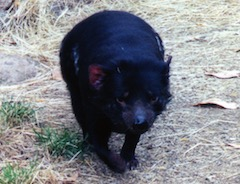
\includegraphics[width=9em]{EigGen/TasmanianDevil}
% AJR's photo of a tasmanian devil.
\end{wrapfigure}
\begin{exercise}  
From the following partial description of the \idx{Tasmanian Devil}, 
Tasmanian Devil
derive a mathematical model in the form \(\yv(t+1)=A\yv(t)\) for the age structure of the Tasmanian Devil.
By finding eigenvalues, and a corresponding eigenvector for each, predict the long-term growth of the population, and predict the long-term relative numbers of Devils of \text{various ages.}

\begin{quoted}{\idx{Wikipedia} 2016, \cite[pp.~64--6]{Owen2005}}
Devils are not monogamous, and their reproductive process is very robust and competitive. 
Males fight one another for the females, and then guard their partners to prevent female infidelity. 
Females can ovulate three times in as many weeks during the mating season, and 80\%~of two-year-old females are seen to be pregnant during the annual mating season. 
Females \idx{average} four breeding seasons in their life and give birth to 20--30 live young after three weeks' gestation. 
The newborn are pink, lack fur, have indistinct facial features and weigh around 0.20\,g (0.0071\,oz) at birth. 
As there are only four nipples in the pouch, competition is fierce and few newborns survive. 
The young grow rapidly and are ejected from the pouch after around 100~days, weighing roughly 200\,g (7.1\,oz). 
The young become independent after around nine months, so the female spends most of her year in activities related to birth and rearing.
\end{quoted}
\end{exercise}






\begin{wrapfigure}l{0pt}
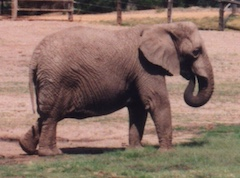
\includegraphics[width=9em]{EigGen/africanElephant}
% AJR's photo of elephant: at Dubbo I think
\end{wrapfigure}
\begin{exercise}  
From the following partial description of the \idx{elephant}, 
derive a mathematical model in the form \(\yv(t+1)=A\yv(t)\) for the age structure of the \idx{elephant}.
By finding eigenvalues, and a corresponding eigenvector for each, predict the long-term growth of the population, and predict the long-term relative numbers of elephants of various ages.

\begin{quoted}{\idx{Wikipedia} 2016 \cite[]{Sukumar2003}}
Gestation in elephants typically lasts around two years with interbirth intervals usually lasting four to five years. Births tend to take place during the wet season. Calves are born 85\,cm (33\,in) tall and weigh around~120\,kg (260\,lb). Typically, only a single young is born, but twins sometimes occur.  The relatively long pregnancy is maintained by five corpus luteums (as opposed to one in most mammals) and gives the foetus more time to develop, particularly the brain and trunk. As such, newborn elephants are precocial and quickly stand and walk to follow their mother and family herd.  A new calf is usually the centre of attention for herd members.  Adults and most of the other young will gather around the newborn, touching and caressing it with their trunks.  For the first few days, the mother is intolerant of other herd members near her young.  Alloparenting---where a calf is cared for by someone other than its mother---takes place in some family groups.  Allomothers are typically two to twelve years old. When a predator is near, the family group gathers together with the calves in the centre.

For the first few days, the newborn is unsteady on its feet, and needs the support of its mother. It relies on touch, smell and hearing, as its eyesight is poor. It has little precise control over its trunk, which wiggles around and may cause it to trip. By its second week of life, the calf can walk more firmly and has more control over its trunk. After its first month, a calf can pick up, hold and put objects in its mouth, but cannot suck water through the trunk and must drink directly through the mouth. It is still dependent on its mother and keeps close to her.

For its first three months, a calf relies entirely on milk from its mother for nutrition after which it begins to forage for vegetation and can use its trunk to collect water.  At the same time, improvements in lip and leg coordination occur.  Calves continue to suckle at the same rate as before until their sixth month, after which they become more independent when feeding.  By nine months, mouth, trunk and foot coordination is perfected.  After a year, a calf's abilities to groom, drink, and feed itself are fully developed.  It still needs its mother for nutrition and protection from predators for at least another year.  Suckling bouts tend to last 2--4\,min/hr for a calf younger than a year and it continues to suckle until it reaches three years of age or older.  Suckling after two years may serve to maintain growth rate, body condition and reproductive ability.  Play behaviour in calves differs between the sexes; females run or chase each other, while males play-fight. The former are sexually mature by the age of nine years while the latter become mature around 14--15 years.  Adulthood starts at about 18~years of age in both sexes.  Elephants have long lifespans, reaching 60--70~years of age.
\end{quoted}
\end{exercise}






\begin{reduce}
\begin{exercise}  
From the following partial description of the \idx{giant mouse lemur}, 
%\marginpar{\includegraphics[width=\marginparwidth]{EigGen/Mirza_zaza}
%\footnotesize\url{https://en.wikipedia.org/wiki/Giant_mouse_lemur}}
% photo from Wikipedia.  Not yet clarified permissions.
derive a mathematical model in the form \(\yv(t+1)=A\yv(t)\) for the age structure of the \idx{giant mouse lemur}.
By finding eigenvalues, and a corresponding eigenvector for each, predict the long-term growth of the population, and predict the long-term relative numbers of \idx{giant mouse lemur}s of \text{various ages.}
\begin{quoted}{\idx{Wikipedia} 2016 \cite[]{Mittermeier2010,Kappeler2005}}
Reproduction starts in November for Coquerel's giant mouse lemur at Kirindy Forest; the estrous cycle runs approximately 22~days, while estrus lasts only a day or less. \ldots

One to three offspring (typically two) are born after 90~days of gestation, weighing approximately 12\,g (0.42\,oz). Because they are poorly developed, they initially remain in their mother's nest for up to three weeks, being transported by mouth between nests. Once they have grown sufficiently, typically after three weeks, the mother will park her offspring in vegetation while she forages nearby. After a month, the young begin to participate in social play and grooming with their mother, and between the first and second month, young males begin to exhibit early sexual behaviors (including mounting, neck biting, and pelvic thrusting). By the third month, the young forage independently, though they maintain vocal contact with their mother and use a small part of her range.

Females start reproducing after ten months, while males develop functional testicles by their second mating season. Testicle size in the northern giant mouse lemur does not appear to fluctuate by season, and is so large relative to the animal's body mass that it is the highest among all primates. This emphasis on sperm production in males, as well as the use of copulatory plugs, suggests a mating system best described as polygynandrous where males use scramble competition (roaming widely to find many females). In contrast, male Coquerel's giant mouse lemurs appear to fight for access to females (contest competition) during their breeding season. Males disperse from their natal range, and the age at which they leave varies from two years to several. Females reproduce every year, although postpartum estrus has been observed in captivity. In the wild, the lifespan of giant mouse lemurs is thought to rarely exceed five or six years
\end{quoted}
\end{exercise}
\end{reduce}




\begin{wrapfigure}l{0pt}
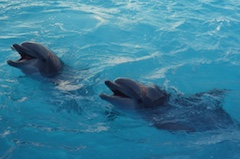
\includegraphics[width=9em]{EigGen/dolphins}
% AJR's photo of two dolphins
\end{wrapfigure}
\begin{exercise}  
From the following partial description of the \idx{dolphin} (Indo-Pacific bottlenose dolphin), 
derive a mathematical model in the form \(\yv(t+1)=A\yv(t)\) for the age structure of the \idx{dolphin}.
(Assume only one calf is born at a time.)
By finding eigenvalues, and a corresponding eigenvector for each, predict the long-term growth of the population, and predict the long-term relative numbers of \idx{dolphin}s of \text{various ages.}

\begin{quoted}{\idx{Wikipedia} 2016 \cite[pp.~362--5]{Reeves2002}}
Indo-Pacific bottlenose dolphins live in groups that can number in the hundreds, but groups of five to 15~dolphins are most common.  In some parts of their range, they associate with the common bottlenose dolphin and other dolphin species, such as the humpback dolphin.

The peak mating and calving seasons are in the spring and summer, although mating and calving occur throughout the year in some regions. Gestation period is about 12~months. Calves are between 0.84 and 1.5~metres (2.8 and~4.9\,ft) long, and weigh between 9 and 21~kilograms (20 and~46\,lb). The calves are weaned between 1.5 and two years, but can remain with their mothers for up to five years. The interbirth interval for females is typically four to six years.

In some parts of its range, this dolphin is subject to predation by sharks; its life span is more than 40~years.
\end{quoted}
\end{exercise}






\begin{exercise}  
You are given that a mathematical model of the age structure of some animal population is
\begin{eqnarray*}
y_1(t+1)&=& 0.5y_1(t)+y_3(t),\\
y_2(t+1)&=& 0.5y_1(t)+0.7y_2(t),\\
y_3(t+1)&=& 0.3y_2(t)+0.9y_3(t).
\end{eqnarray*}
Invent an animal \idx{species}, and time scale, and create details of a plausible scenario for the breeding and life cycle of the species that could lead to this mathematical model.  
Write a coherent paragraph about the breeding and life cycle of the species with enough information that someone could deduce this mathematical model from your description.  
Be creative.
\end{exercise}











\begin{exercise}  
For \(X\) denoting each of the following matrices, find by hand calculation the \idx{eigenvalue}s and \idx{eigenvector}s of the larger matrix~\(\begin{bmat} O&X\\\tr X&O \end{bmat}\).
Show your working.
Relate these to an \svd\ of the particular matrix~\(X\).
\begin{Parts}
\item \(\eAii=\begin{bmatrix} 3\\4 \end{bmatrix}\)
\answer{\(\lambda=0,\pm5\), \((\frac45,-\frac35,0)\) and \((\frac35,\frac45,\pm1)\)}

\item \(\eAii=\begin{bmatrix} -5&12 \end{bmatrix}\)
\answer{\(\lambda=0,\pm13\), \((0,\frac{12}{13},\frac5{13})\) and \((\pm1,-\frac5{13},\frac{12}{13})\)}

\item \(\eAii=\begin{bmatrix} 1&0\\0&-2 \end{bmatrix}\)
\answer{\(\lambda=\pm1,\pm2\), \((\pm1,0,1,0)\) and \((0,1,0,\mp1)\)}

\item \(\eAii=\begin{bmatrix} 0&1\\-4&0 \end{bmatrix}\)
\answer{\(\lambda=\pm1,\pm4\), \((1,0,0,\pm1)\) and \((0,1,\mp1,0)\)}

\end{Parts}
\end{exercise}




\begin{reduce}
\begin{exercise}  
Find by hand calculation all eigenvalues and corresponding eigenvectors of the \idx{generalized eigen-problem} \(A\vv=\lambda B\vv\) for the following pairs of matrices.
Check your calculations with \script.
%\begin{verbatim}
%n=2,A=0+round(randn(n)*2),B=0+round(randn(n)*2),[v,d]=eig(A,B), v*diag(1./v(1,:))
%\end{verbatim}
\begin{enumerate}
\item \(A=\begin{bmatrix} 1 & 3
\\ 0 & 0 \end{bmatrix}\),
\(B=\begin{bmatrix} 0 & 3
\\ 4 & 4 \end{bmatrix}\)
\answer{eigenvalues \(0,\tfrac23\); eigenvectors proportional to \((3,-1),(1,-1)\), respectively}

\item \(A=\begin{bmatrix} -1 & 0
\\ 5 & 1 \end{bmatrix}\),
\(B=\begin{bmatrix} 1 & 2
\\ -1 & -2 \end{bmatrix}\)
\answer{eigenvalue \(\tfrac17\); eigenvectors proportional to \((1,-4)\)}

\item \(A=\begin{bmatrix} 3 & -1
\\ -1 & -2 \end{bmatrix}\),
\(B=\begin{bmatrix} -3 & -3
\\ 1 & -1 \end{bmatrix}\)
\answer{eigenvalues \(-1,\tfrac76\); eigenvectors proportional to \((1,0),(1,-\tfrac{13}6\), respectively}

\item \(A=\begin{bmatrix} 1 & -1
\\ 1 & -4 \end{bmatrix}\),
\(B=\begin{bmatrix} 1 & -0
\\ 2 & -2 \end{bmatrix}\)
\answer{eigenvalues \(1\pm \i/\sqrt2\), eigenvectors proportional to \((1,\mp \i/\sqrt2)\), respectively}

\item \(A=\begin{bmatrix} 0 & 1 & -2
\\ -2 & -1 & -2
\\ 1 & 0 & 2 \end{bmatrix}\),
\(B=\begin{bmatrix} 1 & 0 & 1
\\ 0 & -2 & 1
\\ -1 & -3 & -1 \end{bmatrix}\)
\answer{eigenvalues \(\tfrac73,-2,0\); eigenvectors proportional to \((1,-\tfrac18,-\tfrac{59}{104}),(0,0,1),(1,-1,-\tfrac12)\), respectively}

\item \(A=\begin{bmatrix} 0 & -2 & 1
\\ -4 & 2 & 3
\\ 2 & -2 & -1 \end{bmatrix}\),
\(B=\begin{bmatrix} 0 & 0 & -1
\\ 0 & 0 & -1
\\ -2 & 0 & 0 \end{bmatrix}\)
\answer{eigenvalues \(0,-2\); eigenvectors proportional to \((1,\tfrac12,1),(0,-\tfrac12,1)\), respectively}

\item \(A=\begin{bmatrix} -1 & 1 & -2
\\ -4 & 0 & 3
\\ 0 & -3 & 0 \end{bmatrix}\),
\(B=\begin{bmatrix} -1 & 1 & 1
\\ 5 & -2 & 1
\\ 2 & -2 & -2 \end{bmatrix}\)
\answer{eigenvalue \(-\tfrac{11}2\); eigenvectors proportional to \((15,22,-13)\)}

\item \(A=\begin{bmatrix} -1 & 2 & -1
\\ 0 & -2 & -1
\\ 3 & 2 & 1 \end{bmatrix}\),
\(B=\begin{bmatrix} -1 & 2 & -1
\\ 0 & 2 & 1
\\ 3 & 1 & -2 \end{bmatrix}\)
\answer{eigenvalues \(1,\tfrac{12}{17},-1\); eigenvectors proportional to \((1,0,0),(4,1,-2),(1,-7,-15)\), respectively}

\end{enumerate}
\end{exercise}


%\begin{verbatim}
%n=4,A=0+round(randn(n)*2),B=0+round(randn(n)),[v,d]=eig(A,B), diag(d)'
%\end{verbatim}
\begin{exercise}  
Use \script\ to find and describe all eigenvalues and corresponding eigenvectors of the \idx{generalized eigen-problem} \(A\vv=\lambda B\vv\) for the following pairs of matrices.
\begin{enumerate}
\item \(A=\begin{bmatrix} -2 & 1 & -2 & -2
\\ -2 & 2 & -1 & 0
\\ -1 & 1 & 2 & 1
\\ 1 & -2 & -1 & -1 \end{bmatrix}\),
\(B=\begin{bmatrix} -1 & 0 & -3 & 1
\\ -1 & 1 & -1 & 1
\\ -1 & 1 & 0 & 1
\\ 3 & 5 & 0 & -2 \end{bmatrix}\)
\answer{eigenvalues \(21.72, 1.50, -0.08, -2.15\) \twodp}

\item \(A=\begin{bmatrix} 3 & 1 & -2 & -4
\\ -2 & -3 & -3 & 2
\\ 1 & 1 & 1 & 2
\\ 1 & 2 & 0 & 0 \end{bmatrix}\),
\(B=\begin{bmatrix} -2 & 1 & 1 & 1
\\ 1 & -1 & 1 & -1
\\ 2 & 0 & -1 & 0
\\ 0 & 0 & 1 & 0 \end{bmatrix}\)
\answer{eigenvalues \(-5.26, 1.53, -0.98\) \twodp}

\item \(A=\begin{bmatrix} 0 & 2 & -1 & -1
\\ 0 & 0 & -1 & 0
\\ 3 & -3 & -1 & 1
\\ 2 & -3 & -2 & -3 \end{bmatrix}\),
\(B=\begin{bmatrix} 1 & 2 & 1 & 1
\\ 1 & 0 & 0 & -1
\\ 0 & 0 & 0 & 0
\\ 2 & -1 & -1 & 0 \end{bmatrix}\)
\answer{eigenvalues \(0.73\pm1.13\i, -1.37\) \twodp}

\item \(A=\begin{bmatrix} 4 & 4 & 0 & 3
\\ 1 & -2 & 0 & 1
\\ 0 & 2 & 4 & 2
\\ 0 & 2 & -1 & 1 \end{bmatrix}\),
\(B=\begin{bmatrix} -1 & 2 & -1 & 1
\\ -2 & 2 & 1 & 1
\\ -1 & 0 & 1 & -2
\\ 1 & 1 & 1 & -1 \end{bmatrix}\)
\answer{eigenvalues \(2.74, -2.20, -0.50\pm0.62\i\) \twodp}
  
\end{enumerate}
\end{exercise}


\begin{exercise}  
Use the properties of \idx{determinant}s (\cref{ch:ddm}), and that an \(n\)th~degree polynomial has exactly \(n\)~zeros (when counted according to multiplicity), to explain why the \idx{generalized eigen-problem} \(A\vv=\lambda B\vv\), for real \(n\times n\) matrices~\(A\) and~\(B\), has \(n\)~eigenvalues iff matrix~\(B\) is \idx{invertible}.
\end{exercise}


%\begin{verbatim}
%n=2,A=randn(2);A=0+round(A+A'),B=randn(n);B=0+round(B+B'),[v,d]=eig(A,B)
%\end{verbatim}
\begin{exercise}  
Consider the \idx{generalized eigen-problem} \(A\vv=\lambda B\vv\) and let \(\lambda_1\neq\lambda_2\) be \idx{distinct eigenvalues} with corresponding eigenvectors~\(\vv_1\) and~\(\vv_2\), respectively.
Invent two real \emph{symmetric} matrices~\(A\) and~\(B\) and record your working which demonstrates that although~\(\vv_1\) and~\(\vv_2\) are not orthogonal, nonetheless \(\tr{\vv_1}B\vv_2=0\).
\answer{one possibility is \(A=\protect\begin{bmat} -1&-1\protect\\-1&1 \protect\end{bmat}\) and \(B=\protect\begin{bmat} 1&1\protect\\1&0 \protect\end{bmat}\)} 
\end{exercise}


\begin{exercise} \label{ex:eennmov} 
Consider the \idx{generalized eigen-problem} \(A\vv=\lambda B\vv\) for real \emph{symmetric} \(n\times n\) matrices~\(A\) and~\(B\). 
Let \(\lambda_1\neq\lambda_2\) be \idx{distinct eigenvalues} with corresponding eigenvectors~\(\vv_1\) and~\(\vv_2\), respectively.
Prove that \(\tr{\vv_1}B\vv_2=0\) \text{always holds.}
\end{exercise}


\begin{exercise} \label{ex:eennmre} 
Prove that if both~\(A\) and~\(B\) are real \emph{symmetric} \(n\times n\) matrices, and the eigenvalues of~\(B\) all have the same sign, then the eigenvalues of the \idx{generalized eigen-problem} \(A\vv=\lambda B\vv\) are all real.
Briefly explain why it is necessary to have the proviso that the eigenvalues of~\(B\) are either all positive or \text{all negative.}
\end{exercise}


\begin{exercise}  
In view of the preceding \cref{ex:eennmre},
invent real symmetric matrices~\(A\) and~\(B\) such that the \idx{generalized eigen-problem} \(A\vv=\lambda B\vv\) has nonreal \idx{complex valued} eigenvalues.
% A=[0 1;1 0], B=[1 0;0 -1] suffices, or vice versa.
\end{exercise}



\begin{exercise}  
Explain briefly how the properties established in the previous two 
\cref{ex:eennmov,ex:eennmre} generalize important properties of the standard eigen-problem \(A\xv=\lambda\xv\) for symmetric~\(A\).
\end{exercise}






%\begin{verbatim}
%n=3,dt=0.5
%rs=[1 1/2 1/3 2/3 3/2 1/4 3/4 4/3]
%erat=rs(randperm(length(rs),n))
%[cn,cd]=rat(randn(1,n),0.2);
%[r,t]=meshgrid(erat,(0:2*n-1)*dt);
%f=(r.^t)*(cn./cd)'
%A=hankel(f(2:n+1),f(n+1:2*n))
%B=hankel(f(1:n),f(n:2*n-1))
%lambda=eig(A,B)
%r=log(lambda)/dt
%[U,P]=meshgrid(lambda,0:n-1);
%U=U.^P
%rcond(U)
%c=U\f(1:n)
%expr=exp(r)
%\end{verbatim}
\begin{exercise} 
Consider the specified data values~\fv\ at the specified times, and either by hand or using \script\ fit a sum of exponentials~\eqref{eq:eiddse}, \(f(t)=c_1e^{r_1t}+c_2e^{r_2t}+\cdots+c_ne^{r_nt}\).
Plot the data and the curve you \text{have fitted.}
\begin{Parts}\sloppy
\item For times \(0,1,2,3\) the data values are \(\fv=(3, 2.75, 2.5625, 2.4219)\).%
\answer{\(f=(3/4)^t+2\)}

\item For times \(0,1,2,3\) the data values are \(\fv=(1.5833, 1.3333, 1.3056, 1.4954)\).%
\answer{\(f=\tfrac54(2/3)^t+\tfrac13(3/2)^t\)}

\item For times \(0,2,4,6\) the data values are \(\fv=(-1, 0.222222, 0.172840, 0.085048)\).%
\answer{\(f=-2(1/3)^t+(2/3)^t\)}

\item For times \(0,0.5,1,1.5\) the data values are \(\fv=(1.3, 0.75355, 0.45, 0.27678)\).%
\answer{\(f=\tfrac45(1/4)^t+\tfrac12(1/2)^t\)}

\item For times \(0,1,2,\ldots,5\) the data values are 
\setbox\ajrqrbox\hbox{\qrcode{% f
f=[-1.00000
  0.12500
  0.71875
  1.03906
  1.21680
  1.31885]
}}\marginajrbox%
\[ \fv=\begin{bmatrix} -1.00000
\\ 0.12500
\\ 0.71875
\\ 1.03906
\\ 1.21680
\\ 1.31885 \end{bmatrix}.\]
\answer{\(f=-2(1/2)^t-\tfrac12(3/4)^t+\tfrac32\)}
  
\item For times \(0,1,2,\ldots,5\) the data values are 
\setbox\ajrqrbox\hbox{\qrcode{% f
f=[3.250000
   2.041667
   1.225694
   0.673900
   0.300178
   0.046636]
}}\marginajrbox%
\[ \fv=\begin{bmatrix} 3.250000
\\ 2.041667
\\ 1.225694
\\ 0.673900
\\ 0.300178
\\ 0.046636 \end{bmatrix}.\]
\answer{\(f=3.25(2/3)^t+\tfrac12(3/4)^t-\tfrac12\)}

\needlines7 
\item For times \(0,2,4,\ldots,10\) the data values are 
\setbox\ajrqrbox\hbox{\qrcode{% f
f=[0.16667
    1.38889
    2.72984
    5.81259
   12.88104
   28.87004]
}}\marginajrbox%
\[ \fv=\begin{bmatrix} 0.16667
\\ 1.38889
\\ 2.72984
\\ 5.81259
\\ 12.88104
\\ 28.87004 \end{bmatrix}.\]
\answer{\(f=\tfrac12(3/2)^t-(1/3)^t+\tfrac23(3/4)^t\)}
  
\item For times \(0,0.5,1,\ldots,2.5\) the data values are 
\setbox\ajrqrbox\hbox{\qrcode{% f
f=[0.75000
  0.89846
  1.08333
  1.30323
  1.55903
  1.85343]
}}\marginajrbox%
\[ \fv=\begin{bmatrix} 0.75000
\\ 0.89846
\\ 1.08333
\\ 1.30323
\\ 1.55903
\\ 1.85343 \end{bmatrix}.\]
\answer{\(f=(4/3)^t+\tfrac14(1/2)^t-\tfrac12(3/4)^t\)}
  
\end{Parts}
\end{exercise}



%\begin{verbatim}
%n=4,dt=2
%ws=1+rand(1,n/2),rs=-rand(1,n/2)
%ps=pi*rand(1,n/2),cs=randn(1,n/2)
%ts=(0:2*n-1)'*dt;
%f=0;for k=1:n/2,f=f+cs(k)*exp(rs(k)*ts).*cos(ws(k)*ts+ps(k));end
%f=f
%A=hankel(f(2:n+1),f(n+1:2*n));
%B=hankel(f(1:n),f(n:2*n-1));
%lambda=eig(A,B)
%r=log(lambda)/dt
%U=(lambda.^(0:n-1)).';
%rcond(U)
%c=U\f(1:n);
%expr=exp(r);
%\end{verbatim}
\begin{exercise}  
Consider the specified data values~\fv\ of some decaying \idx{oscillation}s at the specified times (in seconds).
Use \script\ to fit a sum of exponentials~\eqref{eq:eiddse}, \(f(t)=c_1e^{r_1t}+c_2e^{r_2t}+\cdots+c_ne^{r_nt}\).
Confirm your fit reproduces the data values.
What frequencies do you detect in the \text{fitted constants?}
\begin{Parts}
\item  For times \(0,1,2,\ldots,7\) the data values are 
\setbox\ajrqrbox\hbox{\qrcode{% f
f=[-0.153161
   0.484787
  -0.124780
  -0.283690
   0.201896
   0.174832
  -0.200418
  -0.092107]
}}\marginajrbox%
\[ \fv=\begin{bmatrix} -0.153161
\\  0.484787
\\ -0.124780
\\ -0.283690
\\  0.201896
\\  0.174832
\\ -0.200418
\\ -0.092107 \end{bmatrix}.\]
\answer{frequencies \(1.20\) and \(1.70\) radians/sec \twodp}
  
\item  For times \(0,1,2,\ldots,7\) the data values are 
\setbox\ajrqrbox\hbox{\qrcode{% f
f=[1.225432
   0.499044
   0.034164
  -0.093971
  -0.103784
  -0.028558
   0.033825
   0.026439]
}}\marginajrbox%
\[ \fv=\begin{bmatrix} 1.225432
\\  0.499044
\\  0.034164
\\ -0.093971
\\ -0.103784
\\ -0.028558
\\  0.033825
\\  0.026439 \end{bmatrix}.\]
\answer{frequencies \(1.57\) and \(1.16\) radians/sec \twodp}
  
\item  For times \(0,0.5,1,\ldots,3.5\) the data values are 
\setbox\ajrqrbox\hbox{\qrcode{% f
f=[0.0060901
   0.1753701
   0.2385516
   0.1787653
   0.0404368
  -0.0998597
  -0.1742818
  -0.1552607]
}}\marginajrbox%
\[ \fv=\begin{bmatrix} 0.0060901
\\  0.1753701
\\  0.2385516
\\  0.1787653
\\  0.0404368
\\ -0.0998597
\\ -0.1742818
\\ -0.1552607 \end{bmatrix}.\]
\answer{frequencies \(1.94\) and \(1.46\) radians/sec \twodp}
  
\item  For times \(0,2,4,\ldots,14\) the data values are 
\setbox\ajrqrbox\hbox{\qrcode{% f
f=[1.297867
  -0.800035
   0.487305
  -0.285714
   0.161499
  -0.090411
   0.051244
  -0.028936]
}}\marginajrbox%
\[ \fv=\begin{bmatrix} 1.297867
\\ -0.800035
\\  0.487305
\\ -0.285714
\\  0.161499
\\ -0.090411
\\  0.051244
\\ -0.028936 \end{bmatrix}.\]
\answer{frequencies \(1.01\) and \(1.53\) radians/sec \twodp}
  
\end{Parts}
\end{exercise}




% supernova CN1991T perhaps \cite[p.146, Ch.~8]{Pereyra2010}
% days from 2448300 and 20-B, digitised from SN1991T.pdf
%   64.2857    7.2833
%   65.0794    7.5333
%   66.6667    7.8500
%   73.8095    8.2500
%   81.7460    8.1333
%   88.0952    7.6000
%   95.2381    6.8667
%  104.7619    5.9167
%  121.4286    5.4500
%  132.5397    5.2500
%  146.0317    5.0333
%  159.5238    4.8667
% use data 3 to 8, say roughly 8 days apart, and mangle to get real
%\begin{verbatim}
%n=3,dt=8
%f=[0.6543
%   1.5783
%   1.6406
%   0.3678
%   0.05918
%   0.008227]
%A=hankel(f(2:n+1),f(n+1:2*n));
%B=hankel(f(1:n),f(n:2*n-1));
%lambda=eig(A,B)
%r=log(lambda)/dt
%U=(lambda.^(0:n-1)).';
%rcond(U)
%c=U\f(1:n)
%\end{verbatim}
\begin{exercise}  
In astronomy, Type~Ia supernova explode, peaking in luminosity in a few days, and then their luminosity declines over months. 
It is conjectured that the decline is powered by the radioactive decay from radioactive Nickel to Cobalt to Iron.
For the supernova \textsc{sn1991t} six measurements, starting on Julian day 2448366 and taken approximately 8~days apart, give the following luminosity values (in some units) \cite[p.146]{Pereyra2010}:
\setbox\ajrqrbox\hbox{\qrcode{% lumen
f=[0.6543
   1.5783
   1.6406
   0.3678
   0.05918
   0.008227]
}}\marginajrbox%
\begin{equation*}
\fv=\begin{bmatrix} 0.6543
\\ 1.5783
\\ 1.6406
\\ 0.3678
\\ 0.05918
\\ 0.008227 \end{bmatrix}
\end{equation*}
Detect the exponential decay in this supernova data by fitting a sum of exponentials~\eqref{eq:eiddse}, \(f(t)=c_1e^{r_1t}+c_2e^{r_2t}+c_3e^{r_3t}\).
Comment on the result.
\answer{\(f=1459e^{-0.36t}-2044e^{-0.33t}+585e^{-0.27t}\) where \(t\) is days post-2448366; but rcond is very poor!}
\end{exercise}




%\begin{verbatim}
%year=(1944:1993)';
%soi=[-0.03; 0.74; 6.37; -7.28; 0.44; -0.99; 1.32
%6.42; -6.51; 0.07; -1.96; 1.72; 6.49; -5.61
%-0.24; -2.90; 1.92; 6.54; -4.61; -0.47; -3.82
%1.94; 6.56; -3.53; -0.59; -4.69; 1.76; 6.53
%-2.38; -0.59; -5.48; 1.41; 6.41; -1.18; -0.45
%-6.19; 0.89; 6.19; 0.03; -0.16; -6.78; 0.21; 5.84
%1.23; 0.30; -7.22; -0.60; 5.33; 2.36; 0.91 ];
%n=length(year)/2, dt=1
%A=hankel(soi(2:n+1),soi(n+1:2*n));
%B=hankel(soi(1:n),soi(n:2*n-1));
%lambda=eig(A,B)
%r=log(lambda)/dt
%U=(lambda.^(0:n-1)).';
%rcond(U)
%c=U\soi(1:n)
%expr=exp(r);
%\end{verbatim}
\begin{exercise}  
Recall that \cref{eg:orthbapp} introduced the phenomenon of \idx{El Ni\~no} which makes a large impact on the world's weather.
El~Ni\~no is correlated significantly with the difference in atmospheric pressure between Darwin and Tahiti---the so-called \idx{Southern Oscillation Index} (\soi).
\cref{fig:soiRoundData} plots a (`smoothed') yearly \idx{average} \soi\ each year for fifty years up to 1993.
Here detect the cycles in the \soi\ by analysing the plotted data as a sum of exponentials~\eqref{eq:eiddse}, \(f(t)=c_1e^{r_1t}+c_2e^{r_2t}+\cdots+c_ne^{r_nt}\).
\begin{enumerate}
\item Enter the data into \script:
\setbox\ajrqrbox\hbox{\qrcode{% soi
year=(1944:1993)';
soi=[-0.03; 0.74; 6.37; -7.28; 0.44; -0.99; 1.32
6.42; -6.51; 0.07; -1.96; 1.72; 6.49; -5.61
-0.24; -2.90; 1.92; 6.54; -4.61; -0.47; -3.82
1.94; 6.56; -3.53; -0.59; -4.69; 1.76; 6.53
-2.38; -0.59; -5.48; 1.41; 6.41; -1.18; -0.45
-6.19; 0.89; 6.19; 0.03; -0.16; -6.78; 0.21; 5.84
1.23; 0.30; -7.22; -0.60; 5.33; 2.36; 0.91 ];
}}\marginajrbox%
\begin{verbatim}
year=(1944:1993)';
soi=[-0.03; 0.74; 6.37; -7.28; 0.44; -0.99; 1.32
6.42; -6.51; 0.07; -1.96; 1.72; 6.49; -5.61
-0.24; -2.90; 1.92; 6.54; -4.61; -0.47; -3.82
1.94; 6.56; -3.53; -0.59; -4.69; 1.76; 6.53
-2.38; -0.59; -5.48; 1.41; 6.41; -1.18; -0.45
-6.19; 0.89; 6.19; 0.03; -0.16; -6.78; 0.21; 5.84
1.23; 0.30; -7.22; -0.60; 5.33; 2.36; 0.91 ];
\end{verbatim}

\item Use \cref{pro:ei} in \script\ to compute the twenty-five complex rates~\rv\ and twenty-five complex coefficients~\cv\ that fit the data.
% albeit poor rcond

\item Find the four relatively large coefficients, when compared to the relatively small coefficients of magnitude\({}<0.015\).
% should really look at size of c*exp(Re(r)t)---but almost the same

\item Explain why these four coefficients indicate that the \soi\ data appears to be dominantly composed of \idx{oscillation}s with periods about \(5.1\)~years and \(2.5\)~years.
% is the 2.5 year a harmonic of the 5 year oscillation?

\end{enumerate}
\end{exercise}

\end{reduce}










\begin{exercise} 
In a few sentences, answer\slash discuss each of the following.
\begin{enumerate}
\item  Given an \(n\times n\) matrix, what leads to the characteristic polynomial being of \(n\)th~degree?

\item How does the trace of a matrix appear in its characteristic polynomial?

\item What is the importance of the multiplicity of eigenvalues of a matrix?

\item What is the relation between the characteristic polynomial of a matrix and its characteristic equation?

\item Why is it beautifully useful to cater for complex valued eigenvalues and eigenvectors of real matrices arising in real problems?

\item What is the evidence for repeated eigenvalues generally being sensitive to computational and experimental errors?

\item What causes \(\yv(t)=c_1\lambda_1^t\vv_1+c_2\lambda_2^t\vv_2+\cdots+c_m\lambda_m^t\vv_m\) to form a general solution to the evolving system \(\yv(t+1)=A\yv(t)\)?

\item How can the singular values of a matrix arise from an eigen-problem?

\begin{reduce}
\item Describe some scenarios that require fitting a sum of exponentials to data.
\end{reduce}

\end{enumerate}
\end{exercise}

\begin{comment}%{ED498555.pdf}
why, what caused X?
how did X occur?
what-if? what-if-not?
how does X compare with Y?
what is the evidence for X?
why is X important?
\end{comment}




\index{eigenvalue|)}
\index{eigenvector|)}
